\documentclass[titlepage,oneside,openany,10pt]{book}

\usepackage[margin=2cm]{geometry}
%\usepackage{titling}
\usepackage{titlesec}
\titlespacing\chapter{0pt}{0pt plus 4pt minus 2pt}{0pt plus 2pt minus 2pt}
\usepackage{marginnote}
\renewcommand*{\marginfont}{\sffamily\footnotesize}

%\usepackage{intcalc}
\usepackage[nomessages]{fp}
%\ExplSyntaxOn
\usepackage{tabu}
\usepackage{imakeidx}
\usepackage{accents}
\usepackage[utf8]{inputenc} 
\usepackage[T1]{fontenc}
\usepackage{textcomp}
\usepackage{pbox}
\usepackage[linktocpage=true]{hyperref}
\usepackage[all]{hypcap}
\hypersetup{
    colorlinks=false,
    %linkcolor=red,
    urlcolor=black,
    hyperfootnotes=false,
    hypertexnames,
    bookmarks=true % Causes clash if hyperref parameters loaded before bookmark, because bookmark loads hyperref without any parameters
}
%\cfoot{\hyperlink{page.i}{TOC}}
\usepackage{fancyhdr}
%\usepackage{hyperref}
\pagestyle{fancy}
\usepackage[table]{xcolor}
%\usepackage{tcolorbox}
%\tcbset{width=\textwidth,boxrule=0pt,colback=apricot,arc=0pt,auto outer arc,left=0pt,right=0pt,boxsep=5pt}
\renewcommand{\headrulewidth}{0pt}% removes header line
\fancypagestyle{plain}{% for chapter starting pages
  \fancyhf{}% clears header fields
  \lfoot{\hyperlink{contents}{Back to: Table of Contents}}}
\lfoot{\hyperlink{contents}{Back to: Table of Contents}}% links the TOC at the center of the page footer

\usepackage{incgraph,tikz}
\usepackage{pdfpages}
\makeindex[intoc]
\usepackage{xparse}
\ExplSyntaxOn
\NewDocumentCommand {\RoundingUpFunction} { m }
 {
  \fp_eval:n { ceil(#1) }
 }
\ExplSyntaxOff
\usepackage{graphicx}
%\DeclareGraphicsExtensions{.png}
\usepackage{cutwin}
\usepackage{color}
\definecolor{shadecolor}{rgb}{1, 0.8, 0.6}
\usepackage{booktabs}
\usepackage{framed}
\usepackage{tabularx}
\usepackage{multirow}
\usepackage{multicol}
\usepackage{blindtext}

%\titlespacing*{\chapter}{0pt}{-30pt}{20pt}

\newenvironment{oralabswrefwfigwcap}[9] %insert title in first {}, then authors in next {}, then {} location
	{
        \newcommand{\footref}{#4}
        \begin{flushright}
                \underline{\textbf{#5}}
        \end{flushright}
        \textbf{#1}\\%include title
        #2\\%include name
        \textit{#3}\\\\%include location
	\FPeval{\cutw}{clip(16.7-#7)}
	\FPeval{\cutj}{clip(#8*2.86+1)}
	%\FPeval{\cutl}{clip(\cutj+1)}
        \def\windowpagestuff{\centering
                \includegraphics[width=#7cm,height=#8cm,keepaspectratio]{#6}\\
		#9
	}
        \opencutright
        \begin{cutout}{0}{\cutw cm}{0pt}{\RoundingUpFunction{\cutj}}
        \noindent
	}
	{
	\end{cutout}
	\vspace{0.5cm}
	\noindent \footref \\ \noindent\rule{15cm}{0.5pt}%\hline
	}

\newenvironment{oralabswrefwfig}[8] %insert title in first {}, then authors in next {}, then {} location
        {
        \newcommand{\oralref}{#5}
	\FPeval{\cutw}{clip(16.7-#7)}
	\FPeval{\cutl}{round(#8/0.35,3)}
        \begin{flushright}
                \underline{\textbf{#4}}
        \end{flushright}
        \textbf{#1}\\%include title
        #2\\%include name
        \textit{#3}\\\\%include location
        \def\windowpagestuff{\centering
                \includegraphics[width=#7cm,height=#8cm,keepaspectratio]{#6}}
        \opencutright
        \begin{cutout}{0}{\cutw cm}{0pt}{\RoundingUpFunction{\cutl}}
        \noindent
        }
        {
        \end{cutout}
        \vspace{0.5cm}
        \noindent \oralref \\ \noindent\rule{15cm}{0.5pt}%\hline
        }

\newenvironment{oralabswref}[5] %insert title in first {}, then authors in next {}, then {} location
        {
        \newcommand{\oralref}{#5}
        \begin{flushright}
                \underline{\textbf{#4}}
        \end{flushright}
        \textbf{#1}\\%include title
        #2\\%include name
        \textit{#3}\\\\%include location
        }
        {
        \vspace{0.5cm}
        \\\noindent \oralref \\ \noindent\rule{15cm}{0.5pt}%\hline
        }

\newenvironment{oralabswfig}[7] %insert title in first {}, then authors in next {}, then {} location
        {
	\FPeval{\cutw}{clip(16.7-#6)}
	\FPeval{\cutl}{round(#7/0.35,3)}
        \begin{flushright}
                \underline{\textbf{#4}}
        \end{flushright}
        \textbf{#1}\\%include title
        #2\\%include name
        \textit{#3}\\\\%include location
        \def\windowpagestuff{\flushright
                \includegraphics[width=#6cm,height=#7cm,keepaspectratio]{#5}}
        \opencutright
        \begin{cutout}{0}{\cutw cm}{0pt}{\RoundingUpFunction{\cutl}}
        \noindent
        }
        {
        \end{cutout}
        %\vspace{0.5cm}
        \noindent\rule{15cm}{0.5pt}%\hline
        }

\newenvironment{oralabswfigwcap}[8] %insert title in first {}, then authors in next {}, then {} location
        {
	\FPeval{\cutw}{clip(16.7-#6)}
	\FPeval{\cutl}{round(#7/0.35,3)}
        \begin{flushright}
                \underline{\textbf{#4}}
        \end{flushright}
        \textbf{#1}\\%include title
        #2\\%include name
        \textit{#3}\\\\%include location
        \def\windowpagestuff{\flushright
                \includegraphics[width=#6cm,height=#7cm,keepaspectratio]{#5}}\\
		#8
        \opencutright
        \begin{cutout}{0}{\cutw cm}{0pt}{\RoundingUpFunction{\cutl}}
        \noindent
        }
        {
        \end{cutout}
        \vspace{0.5cm}
        \noindent\rule{15cm}{0.5pt}%\hline
        }

\newenvironment{oralabs}[4] %insert title in first {}, then authors in next {}, then {} location
        {
        \begin{flushright}
                \underline{\textbf{#4}}
        \end{flushright}
        \textbf{#1}\\%include title
        #2\\%include name
        \textit{#3}\\\\%include location
        }
        {
        \\
	%\vspace{0.5cm}
        \noindent\rule{15cm}{0.5pt}%\hline
        }

\newenvironment{oralabskeynote}[3]
        {
        \vspace{0.3cm}
        \noindent\textbf{#1}\\%include title
        #2\\%include name
        \textit{#3}\\\\%include location
        }
        {
        \\
	%\vspace{0.5cm}
        \noindent\rule{15cm}{0.5pt}%\hline
        }

\newenvironment{oralabswfigkeynote}[6]
        {
	\FPeval{\cutw}{clip(16.7-#5)}
	\FPeval{\cutl}{round(#6/0.35,3)}
        \noindent\textbf{#1}\\%include title
        #2\\%include name
        \textit{#3}\\ %include location
        \def\windowpagestuff{\flushright
                \includegraphics[width=#5cm,height=#6cm,keepaspectratio]{#4}}
        \opencutright
        \begin{cutout}{0}{\cutw cm}{0pt}{\RoundingUpFunction{\cutl}}
        \noindent
        }
        {
        \end{cutout}
        %\vspace{0.5cm}
        \noindent\rule{15cm}{0.5pt}%\hline
        }

%~~~~~~~~~~~~~~~~~~~~~~~~~~~~~~~~~~~~~~~~~~~~~~~~~~

%insert title in first {}, then authors in next {}, then {} location
\newenvironment{posterabswrefwfigwcap}[9] 
        {
        \newcommand{\footref}{#5}
	\FPeval{\cutw}{clip(16.7-#7)}
	\FPeval{\cutl}{round(#8/0.35+1,3)}
	\begin{flushright}
                \underline{\textbf{#4}}
        \end{flushright}
        \textbf{#1}\\%include title
        #2\\%include name
        \textit{#3}\\\\%include location
        \def\windowpagestuff{\centering
                \includegraphics[width=#7cm,height=#8cm,keepaspectratio]{#6}\\
		#9
	}
        \opencutright
        \begin{cutout}{0}{\cutw cm}{0pt}{\RoundingUpFunction{\cutl}}
        \noindent
	}
	{
	\end{cutout}
	\vspace{0.5cm}
	\noindent \footref \\ \noindent\rule{15cm}{0.5pt}%\hline
        }

\newenvironment{posterabswrefwfig}[8] %insert title in first {}, then authors in next {}, then {} location
        {
        \newcommand{\posterref}{#5}
	\FPeval{\cutw}{clip(16.7-#7)}
	\FPeval{\cutl}{round(#8/0.35+1,3)}
	\begin{flushright}
                \underline{\textbf{#4}}
        \end{flushright}
        \textbf{#1}\\%include title
        #2\\%include name
        \textit{#3}\\\\%include location
        \def\windowpagestuff{\centering
                \includegraphics[width=#7cm,height=#8cm,keepaspectratio]{#6}
	}
        \opencutright
        \begin{cutout}{0}{\cutw cm}{0pt}{\RoundingUpFunction{\cutl}}
        \noindent
	}
	{
	\end{cutout}
	\vspace{0.5cm}
	\\\noindent \posterref \\ \noindent\rule{15cm}{0.5pt}%\hline
        }

\newenvironment{posterabswref}[5] %insert title in first {}, then authors in next {}, then {} location
        {
        \newcommand{\posterref}{#5}
	\begin{flushright}
                \underline{\textbf{#4}}
        \end{flushright}
        \textbf{#1}\\%include title
        #2\\%include name
        \textit{#3}\\\\%include location
        }
        {
        \vspace{0.5cm}
        \\\noindent \posterref \\ \noindent\rule{15cm}{0.5pt}%\hline
        }

\newenvironment{posterabswfig}[7] %insert title in first {}, then authors in next {}, then {} location
        {
	\FPeval{\cutw}{clip(16.7-#6)}
	\FPeval{\cutl}{round(#7/0.35+1,3)}
	\begin{flushright}
                \underline{\textbf{#4}}
        \end{flushright}
        \textbf{#1}\\%include title
        #2\\%include name
        \textit{#3}\\\\%include location
        \def\windowpagestuff{\centering
                \includegraphics[width=#6cm,height=#7cm,keepaspectratio]{#5}
	}
        \opencutright
        \begin{cutout}{0}{\cutw cm}{0pt}{\RoundingUpFunction{\cutl}}
        \noindent
	}
	{
	\end{cutout}
	\noindent\rule{15cm}{0.5pt}%\hline
        }

\newenvironment{posterabswfigwcap}[8] %insert title in first {}, then authors in next {}, then {} location
        {
	\FPeval{\cutw}{clip(16.7-#6)}
	\FPeval{\cutl}{round(#7/0.35+1,3)}
	\begin{flushright}
                \underline{\textbf{#4}}
        \end{flushright}
        \textbf{#1}\\%include title
        #2\\%include name
        \textit{#3}\\\\%include location
        \def\windowpagestuff{\centering
                \includegraphics[width=#6cm,height=#7cm,keepaspectratio]{#5}\\
		#8
	}
        \opencutright
        \begin{cutout}{0}{\cutw cm}{0pt}{\RoundingUpFunction{\cutl}}
        \noindent
	}
	{
	\end{cutout}
	\noindent\rule{15cm}{0.5pt}%\hline
        }

\newenvironment{posterabs}[4] %insert title in first {}, then authors in next {}, then {} location
        {
	\begin{flushright}
                \underline{\textbf{#4}}
        \end{flushright}
        \textbf{#1}\\%include title
        #2\\%include name
        \textit{#3}\\\\%include location
        }
        {
        \\
        \noindent\rule{15cm}{0.5pt}%\hline
        }

%~~~~~~~~~~~~~~~~~~~~~~~~~~~~~~~~~~~~~~~~~~~~~~~~~~
%%% Title page %%%

\title{
    
\includegraphics[width=12cm,keepaspectratio]
    {Other_Figures/owl_bw.png}\\
    \vspace{2cm}
    Program Guide}
\author{
    \textbf{Chemical Biophysics Symposium}\\
    University of Toronto\\
    Toronto, Ontario\\
    Canada\\\\
    
    % TODO: needs updating
    \textbf{Contact Information:}\\
    Alexander Sever (Student Co-Chair): 
    \underline{alexander.sever@mail.utoronto.ca} \\
    Mirna Ghattas (Student Co-Chair): 
    \underline{mirna.ghattas@mail.utoronto.ca}\\
    Professor Cynthia Goh (Faculty Advisor): 
    \underline{cynthia.goh@utoronto.ca}\\\\
    Cover image by: Michael Nosella (photo), Rosie Irwin (design)}
% TODO: $time
\date{April 28-30, 2023}

%%% End of title page %%%
%~~~~~~~~~~~~~~~~~~~~~~~~~~~~~~~~~~~~~~~~~~~~~~~~~~

% TODO: what is this? -- Has to do with options for display in table of contents; should it be here?
\setcounter{tocdepth}{5}

\begin{document}

\incgraph[paper=current][width=\paperwidth,keepaspectratio]{Other_Figures/program_cover.png}
\maketitle
\frontmatter

\hypertarget{contents}{}
\renewcommand\contentsname{Table of Contents}
\tableofcontents  

%~~~~~~~~~~~~~~~~~~~~~~~~~~~~~~~~~~~~~~~~~~~~~~~~~~~~~~~~~~~~~~~~~~~~
%====================================================================
%~~~~~~~~~~~~~~~~~~~~~~~~~~~~~~~~~~~~~~~~~~~~~~~~~~~~~~~~~~~~~~~~~~~~
  
\chapter*{Message from the Chairs}
\label{chapter:message_from_the_chair}
%\cleardoublepage
\phantomsection\addcontentsline{toc}{chapter}{\hyperref[chapter:message_from_the_chair]{Message from the Chairs}}

\vspace{1cm}
Welcome to the 19$^{\textrm{th}}$ annual Chemical Biophysics Symposium!  After a tough couple of years, we are so excited to host CBP again! Our committee has worked so hard all year to bring you another excellent iteration of the conference. CBP provides a unique forum for researchers around the world to discuss enticing and interdisciplinary topics along the interface of Chemistry, Biology and Physics. We are pleased to continue this tradition at CBP2023, and aim to foster an intimate atmosphere, for you to seize opportunities to discuss and share different perspectives, from a variety of disciplines with your fellow researchers.\\\

Over the course of the weekend, we encourage you to take advantage of all the symposium has to offer! The weekend is packed with inspiring talks from our keynote speakers and exciting research from our contributed talks and poster presentations. The conference begins with a tutorial on Friday morning hosted by our \textbf{\textit{Gold sponsor}}, AOMF, and a product booth from our \textbf{\textit{Silver sponsor}}, Mandel. A set of workshops are offered by SciNet to give a hands-on introduction on the rapidly expanding field of Neural Nets; and scientists from Lumira, ProteinQure, and Sanofi, are also here to talk about the business of science, and how to make the transition. For years, CBP has featured a Friday night panel to foster discussion and debate amongst attendees. In our continual pursuit of creating a dynamic symposium, we are excited to introduce invited panelists to discuss \textit{the communication of science}, and the challenges we face in modern society to achieve effective communication. We have invited four experts who are coming together from the writing industry, scientific institutions, and academia for what we expect to be a beneficial and thought-provoking panel discussion.\\\

On behalf of the CBP Executive Committee, we extend a sincere gratitude to our keynote speakers, workshop presenters, and panelists for engaging us and attendees alike. In addition, we would like to acknowledge the substantial support from both our academic and industry sponsors which made this event possible and allowed us to fulfill our vision. Our sponsors have given us the means to host CBP annually since 2002, and they continue to be a foundation for our chance to improve the quality of the symposium year after year.\\\

Finally, the success of the 19$^{\textrm{th}}$ annual Chemical Biophysics Symposium depends on the efforts of our incredible executive committee. They have dedicated a great deal of time to ensure the conference is fun and engaging to everyone. Their genuine excitement and effort towards planning the symposium, has made it a truly phenomenal team to be a part of. We hope you find CBP2023 to be a memorable and exciting experience. Please feel free to approach the committee with any questions, comments, or concerns that you may have. Have a hoot of a weekend and remember to share on socials with \#CBP2023! We look forward to seeing you again in 2024!\\\

\textbf{Alexander Sever \& Mirna Ghattas}\\ 
Co-Chairs, Chemical Biophysics Symposium 2023

%~~~~~~~~~~~~~~~~~~~~~~~~~~~~~~~~~~~~~~~~~~~~~~~~~~~~~~~~~~~~~~~~~~~~
%====================================================================
%~~~~~~~~~~~~~~~~~~~~~~~~~~~~~~~~~~~~~~~~~~~~~~~~~~~~~~~~~~~~~~~~~~~~

% TODO: is it possible to automate insertion of logos?
\chapter*{Our Sponsors -- \textit{Thank you!}}
\label{chapter:sponsors}
%\markboth{Abstracts: Poster Presentations}{}
\phantomsection\addcontentsline{toc}{chapter}{\hyperref[chapter:sponsors]{Our Sponsors}}

\begin{center}%[h]
	
\includegraphics[width=\textwidth,keepaspectratio]{Other_Figures/sponsors_withtiers.jpg}
\end{center}

%~~~~~~~~~~~~~~~~~~~~~~~~~~~~~~~~~~~~~~~~~~~~~~~~~~~~~~~~~~~~~~~~~~~~
%====================================================================
%~~~~~~~~~~~~~~~~~~~~~~~~~~~~~~~~~~~~~~~~~~~~~~~~~~~~~~~~~~~~~~~~~~~~

\chapter*{Executive Committee}
\label{chapter:executive_committee}  
  
\phantomsection\addcontentsline{toc}{chapter}{\hyperref[chapter:executive_committee]{Executive Committee}}

% TODO: is there a better environment for this?
% TODO: needs updating
\begin{multicols}{2}
    \fontsize{12pt}{12pt}\selectfont
    \noindent\textbf{Student Co-Chairs}\\
    Alexander Sever\\
    Mirna Ghattas\\
    \\
    \noindent\textbf{Finance}\\
    Zi Hao (Nemo) Liu\\
    \\
    \noindent\textbf{Publicity \& Communications}\\
    Mahrukh Fatima\\
    Samantha Sanayhie\\
    \\
    \noindent\textbf{Website \& Graphics}\\
    Zhi Wei (Wilson) Zeng\\                          		
    Rosie Irwin\\							        
    Zi Hao (Nemo) Liu\\
    \\
    \noindent\textbf{Workshops}\\
    James Otis\\
    \\
    \noindent\textbf{Speaker Coordination}\\
    James Otis\\
    Max Reed\\
    Zhengkun Chen\\
    Alexander Sever\\
    Mahrukh Fatima\\
    \\
    \noindent\textbf{Panel Discussion}\\
    James Otis\\
    Rosie Irwin\\
    \\
    \noindent\textbf{General Executive}\\
    Logan Zettle\\
    Xenia Fernandes\\
    Thomas Tsangaris\\
    \\\\
    \noindent\textbf{Sponsorship}\\
    James Otis\\
    Randy Yoo\\
    Naimul Hasan\\
    \\
    \noindent\textbf{Food \& Beverage}\\
    Zhengkun Chen\\
    Mirna Ghattas\\
    Alexander Sever\\
    \\
    \noindent\textbf{Logistics}\\
    Max Reed\\
    Mark Croxall\\
    James Otis\\
    \\
    \noindent\textbf{Program}\\
    Zhi Wei (Wilson) Zeng\\
    Mark Croxall\\
    Mirna Ghattas\\
    \\
    \noindent\textbf{Merchandise}\\
    Rosie Irwin\\
    \\
    \noindent\textbf{Art \& Design}\\
    Rosie Irwin\\
    Zi Hao (Nemo) Liu\\
    \\
    \textbf{Student Advisor}\\
    Samantha McWhirter\\
    \\
    \noindent\textbf{Faculty Advisors}\\
    Prof. M. Cynthia Goh\\
    Prof. David McMillen\\
    \\\
\end{multicols}

%~~~~~~~~~~~~~~~~~~~~~~~~~~~~~~~~~~~~~~~~~~~~~~~~~~~~~~~~~~~~~~~~~~~~
%====================================================================
%~~~~~~~~~~~~~~~~~~~~~~~~~~~~~~~~~~~~~~~~~~~~~~~~~~~~~~~~~~~~~~~~~~~~

\chapter*{Symposium Schedule}
\label{chapter:schedule}
\markboth{Symposium Schedule}{}
%
\phantomsection\addcontentsline{toc}{chapter}{\hyperref[chapter:schedule]{Symposium Schedule}}
%
\section*{\textbf{Lash Miller Chemical Laboratories}\\University of Toronto\\\textit{80 St. George Street}}
%
%~~~~~~~~~~~~~~~~~~~~~~~~~~~~~~~~~~~~~~~~~~~~~~~~~~~~~~~~~~~~~~~~~~~~
%
\newpage
\section*{\textbf{Friday, April 28th, 2023}}
\label{sec:day1}
\phantomsection\addcontentsline{toc}{section}{\hyperref[sec:day1]{Friday, April 28th}}

\begin{center}
% TODO: HIGH PRIORITY. There has to be a better environment for this. Overhaul the environment.
\begin{tabular}{  c  m{9.8cm}  c  }
\toprule
10:30AM - 3:00PM 			& {\textbf{Registration}} 		&  \textbf{Main Lobby} \\
\midrule
11:15AM - 12:15PM 			& \cellcolor[HTML]{FFD700}
						\begin{tabular}[l]{@{}l@{}}
        						\textbf{\underline{Sponsor Workshop}:}\\\textbf{Advanced Optical Microscopy Facility (AOMF)}\\
        						Tutorial: Guidance for Confocal Microscopy\\
                                (Lunch provided to attendees)
						\end{tabular}
												&	\textbf{LM155}\\
\midrule
12:30PM - 3:15PM 			& \cellcolor[HTML]{CCCCCC}
						\begin{tabular}[l]{@{}l@{}}
        						\textbf{\underline{Workshop}:}\\
						\textbf{SciNet}\\
        						Introduction to Neural Nets
						\end{tabular}
												& \textbf{LM155}\\
\midrule
12:30PM - 3:15PM 			& \cellcolor[HTML]{CCCCCC}
						\begin{tabular}[l]{@{}l@{}}
        						\textbf{\underline{Workshop}:}\\
						\textbf{Baye Galligan (Lumira), Tracy Stone (ProteinQure),}\\ \textbf{Shaolong Zhu \& Andrew James (Sanofi)}\\
        						The Business of Science
						\end{tabular}
												& \textbf{LM157}\\

\midrule
3:15PM - 3:25PM 			& Coffee Break 			& \begin{tabular}[c]{@{}c@{}} 
													Sponsored by\\
													\textbf{Mandel}\\Main Lobby
													\end{tabular} \\
\midrule
3:30PM - 3:50PM 			& Opening Remarks 
						- \textbf{Alexander Sever and Mirna Ghattas}	 	& \textbf{LM162}\\
\midrule
\textbf{\underline{Session I}}\vspace{0.2cm} 
					 	& \textbf{Chair:} Logan Zettle
												&  \\
3:50PM - 4:50PM 			& 
						\cellcolor[HTML]{ffcc99}
						\begin{tabular}[l]{@{}l@{}} 
						\textbf{Prof. Leyla Soleymani} (\textit{McMaster University})\\
						Hierarchical functional surfaces for biological sensing and \\pathogen repellency
						\end{tabular} 				& \\ 
4:50PM - 5:10PM 			& \vspace{0.1cm} 
						\begin{tabular}[l]{@{}l@{}} 
						\textbf{Elnaz Samani} (\textit{University of Toronto})\\
						Investigating Acyl Carrier Protein Shuttling Pathways in\\Fungal Fatty Acid Synthase
						\end{tabular} 				& \textbf{LM162}\\
5:10PM - 5:30PM 			& \vspace{0.1cm} 
						\begin{tabular}[l]{@{}l@{}} 
						\textbf{Ilya Yakavets } (\textit{University of Toronto})\\
						Microfluidic Spheroid-on-a-chip model for screening of liposome\\internalization in solid tumors 
						\end{tabular} 				& \\

5:30PM - 5:50PM 			& \vspace{0.1cm} 
						\begin{tabular}[l]{@{}l@{}} 
						\textbf{Matthew Gerry} (\textit{University of Toronto})\\
						A new role for the proton motive force in bacterial efflux pumps
						\end{tabular} 				& \\
\midrule
5:50PM - 6:15PM 			& Coffee Break			
												& \begin{tabular}[c]{@{}c@{}} 
													Sponsored by\\
													\textbf{Mandel}\\Main Lobby
													\end{tabular} \\
\midrule

6:15PM - 7:30PM 			& \cellcolor[HTML]{CCCCCC}
						\begin{tabular}[l]{@{}l@{}} 
						\underline{\textbf{Panel Discussion:}} Science Communication in Modern Society\vspace{0.1cm}\\ 
						\hspace{0.5cm}\textbf{Moderators:} James Otis \& Rosie Irwin\\
						\hspace{0.5cm}\textbf{Panelists:} Prof. Christine Bear, Dr. Fiona Coll, \\
						\hspace{2.23cm} Prof. Dwayne Miller, Maria Medeleanu
						\end{tabular} 		
												& \textbf{LM162}\\
\midrule
7:30PM - 10:00PM 			& \textbf{\underline{Networking Dinner}} 
												& \begin{tabular}[c]{@{}c@{}} \textbf{Davenport Atrium}\\Lash Miller \end{tabular}\\
\bottomrule
\end{tabular}
\end{center}

%~~~~~~~~~~~~~~~~~~~~~~~~~~~~~~~~~~~~~~~~~~~~~~~~~~~~~~~~~~~~~~~~~~~~

\section*{\textbf{Saturday, April 29th, 2023}}
\label{sec:day2}
\phantomsection\addcontentsline{toc}{section}{\hyperref[sec:day2]{Saturday, April 29th}}

\begin{tabular}{  c  m{10.2cm}  c  }
\toprule
8:15AM - 9:00AM 			& \underline{\textbf{Breakfast:}} Pastries \& Refreshments
												&  \begin{tabular}[c]{@{}c@{}} Sponsored by\\\textbf{AOMF}\\Main Lobby\end{tabular}\\
\midrule
\textbf{\underline{Session II}}\vspace{0.2cm} 
					 	& \textbf{Chair:} Alexander Sever
												&  \\
9:00AM - 10:00AM 			& 
						\cellcolor[HTML]{ffcc99}
						\begin{tabular}[l]{@{}l@{}} 
						\textbf{Prof. Karen Fleming} (\textit{Johns Hopkins University})\\
						Chaperoning Unfolded Outer Membrane Proteins
						\end{tabular} 				& \begin{tabular}[c]{@{}c@{}}  \end{tabular}\\ 
10:00AM - 10:20AM 			& \vspace{0.14cm} 
						\begin{tabular}[l]{@{}l@{}} 
						\textbf{Dr. Robert Harkness} (\textit{University of Toronto})\\
						Flexible client-dependent cages in the assembly landscape of \\the periplasmic protease-chaperone DegP
						\end{tabular}  &  \begin{tabular}[c]{@{}c@{}}\\\\\textbf{LM162} \end{tabular}\\
10:20AM - 10:40AM 			& \vspace{0.14cm} 
						\begin{tabular}[l]{@{}l@{}} 
						\textbf{Navid Afrasiabian} (\textit{Western University})\\
						Promoting single-file capture by pulley effect
						\end{tabular} 				& \begin{tabular}[c]{@{}c@{}}    \end{tabular}\\
10:40AM - 11:00AM 			& \vspace{0.14cm} 
						\begin{tabular}[l]{@{}l@{}} 
						\textbf{Junyeong Kim} (\textit{Toronto Metropolitan University})\\
						Modelling diffusive protein target search in endoplasmic\\reticulum tubes
						\end{tabular} 				& \begin{tabular}[c]{@{}c@{}}    \end{tabular}\\
\midrule
11:00AM - 11:15AM 			& \textbf{Coffee Break}
												& \textbf{Main Lobby}\\

\midrule
\textbf{\underline{Session III}}\vspace{0.2cm} 
					 	& \textbf{Chair:} Mirna Ghattas	
												&  \\
%
11:15AM - 12:15PM 			& 
						\cellcolor[HTML]{ffcc99}
						\begin{tabular}[l]{@{}l@{}} 
						\textbf{Prof. Christine Mayr} (\textit{Sloan Kettering Institute})\\
						mRNAs control the conformations of proteins with disordered\\regions
						\end{tabular}				& \\
12:15PM - 12:35PM 			& \vspace{0.12cm} 
						\begin{tabular}[l]{@{}l@{}} 
						\textbf{Prof. Steffen Lindert} (\textit{Ohio State University})\\
						Mechanism of Calcium Sensitivity Modulation of Cardiac Troponin\\C by Small Molecules Illuminated by Umbrella Sampling\\Simulations
						\end{tabular} 				& \begin{tabular}[c]{@{}c@{}} \\\\\\\textbf{LM162} \end{tabular}\\
12:35PM - 12:55PM 			& \vspace{0.12cm} 
						\begin{tabular}[l]{@{}l@{}} 
						\textbf{Bruna Siebeneichler} (\textit{University of Waterloo})\\
						Elucidating inclusion body structure formed by an $\alpha$-helix protein
						\vspace{0.14cm} 
						\end{tabular} 				& \\
12:55PM - 1:15PM 			& \vspace{0.12cm} 
						\begin{tabular}[l]{@{}l@{}} 
						\textbf{Carlos Castillo Orellana} (\textit{Queen's University})\\
						Non-bonded parameters for biological force field derived from\\Atom-in-molecules approaches
						\vspace{0.14cm} 
						\end{tabular} 				& \\
\midrule
1:15PM - 1:45PM 			& \textbf{Lunch}
												& \textbf{Main Lobby}\\

\midrule

1:45PM - 3:00PM 			& \cellcolor[HTML]{CCCCCC}\textbf{Poster Session A} -- Odd numbers
												& \textbf{Main Lobby}\\
\midrule

3:00PM - 4:15PM 			& \cellcolor[HTML]{CCCCCC}\textbf{Poster Session B} -- Even Numbers				& \textbf{Main Lobby}\\
\midrule
\textbf{\underline{Session IV}}\vspace{0.2cm} 
					 	& \textbf{Chair:} Zhengkun (Zicor) Chen
												& \\
%
4:30PM - 5:30PM 			& 
						\cellcolor[HTML]{ffcc99}
						\begin{tabular}[l]{@{}l@{}} 
						\textbf{Prof. Anna Taubenberger} (\textit{TU Dresden})\\
						Mapping cell volume and mechanical changes within tumor\\spheroids under confinement
						\end{tabular}				& \\
5:30PM - 5:50PM 			& \vspace{0.14cm}
						\begin{tabular}[l]{@{}l@{}} 
						\textbf{Prof. Sarah Rauscher} (\textit{University of Toronto Mississauga})\\
						Protein Dynamics in a Crystal are Functionally Relevant
						\vspace{0.12cm} 
						\end{tabular} 				&  \\
5:50PM - 6:10PM 			& \vspace{0.14cm} 
						\begin{tabular}[l]{@{}l@{}} 
						\textbf{Dr. Manoel L. da Silva-Neto} (\textit{University of Toronto})\\
						Ultrasound-imaging of Picosecond Infrared Laser Ablation
						\vspace{0.12cm} 
						\end{tabular} 				&\textbf{LM162}\\
6:10PM - 6:30PM 			& \vspace{0.14cm}
						\begin{tabular}[l]{@{}l@{}} 
						\textbf{Michael Fish} (\textit{Wilfrid Laurier University})\\
						TOC159 Receptors are Anchored in the Chloroplast Outer\\Envelope by a $\beta$-Barrel and Targeted Using a Bi-Partite\\Signal at the C-Terminus
						\vspace{0.14cm} 
						\end{tabular} 				&  \\

\midrule
7:30PM - onwards			& \textbf{\underline{Banquet Dinner}} 
												& \begin{tabular}[c]{@{}c@{}} \textbf{Dim Sum King}\\421 Dundas St. W\end{tabular}\\
\bottomrule
\end{tabular}

%~~~~~~~~~~~~~~~~~~~~~~~~~~~~~~~~~~~~~~~~~~~~~~~~~~~~~~~~~~~~~~~~~~~~
 
\section*{\textbf{Sunday, April 30th, 2023}}
\label{sec:day3}
\phantomsection\addcontentsline{toc}{section}{\hyperref[sec:day3]{Sunday, April 30th}}

\begin{tabular}{  c  m{10cm}  c  }
\toprule
8:15AM - 9:00AM 			& \underline{\textbf{Breakfast:}} Pastries \& Refreshments
												& \textbf{Main Lobby}\\
\midrule
\textbf{\underline{Session V}}\vspace{0.2cm} 
					 	& \textbf{Chair:} Mahrukh Fatima
												&  \\
9:00AM - 10:00AM 			& 
						\cellcolor[HTML]{ffcc99}
						\begin{tabular}[l]{@{}l@{}} 
						\textbf{Prof. Kevin Gardner} (\textit{City College of New York})\\
						Transforming nature’s switches into our biotech tools and\\therapeutics
						\end{tabular} 				& \\ 
10:00AM - 10:20AM 			& \vspace{0.14cm} 
						\begin{tabular}[l]{@{}l@{}} 
						\textbf{Prof. Claudiu Gradinaru } (\textit{University of Toronto Mississauga})\\
						Illuminating disorder and dynamics in proteins with\\single-molecule tools
						\end{tabular} 			& \\
10:20AM - 10:40AM 			& \vspace{0.14cm} 
						\begin{tabular}[l]{@{}l@{}} 
						\textbf{Zhi Wei Zeng} (\textit{University of Toronto})\\
						Ion permeation mechanism of Cystic Fibrosis Transmembrane\\Conductance Regulator (CFTR)
						\end{tabular} 				& \textbf{LM162}\\
10:40AM - 11:00AM 			& \vspace{0.14cm} 
						\begin{tabular}[l]{@{}l@{}} 
						\textbf{Divya Kriti} (\textit{University of British Columbia})\\
						A systematic strategy to link human genetic variations to\\drug response
                        \vspace{0.14cm} 
						\end{tabular} 				& \\
\midrule
11:00AM - 11:20AM 			& Coffee Break					
												& \begin{tabular}[c]{@{}c@{}} \textbf{Main Lobby}  \end{tabular}\\
\midrule
\textbf{\underline{Session VI}}\vspace{0.2cm} 
					 	& \textbf{Chair:} Max Reed
												&  \\
%
11:20AM - 12:20PM 			& \vspace{0.14cm}
                        \cellcolor[HTML]{ffcc99}
						\begin{tabular}[l]{@{}l@{}} 
						\textbf{Prof. Haissi Cui} (\textit{University of Toronto})\\
						Genetic code interpretation in mammalian organisms
						\end{tabular}				& \begin{tabular}[c]{@{}c@{}} \end{tabular}\\
						
12:20PM - 12:40PM 		& \vspace{0.14cm}
                        \begin{tabular}[l]{@{}l@{}} 
						\textbf{Sarah Bickers} (\textit{University of Toronto})\\
						Structural Studies Probing the Role of Phosphorylation of the\\Intrinsically Disordered Regulatory Region of the Yeast\\Cadmium Factor 1 Protein
						\end{tabular} 				& \\
12:40PM - 1:00PM 			& \vspace{0.14cm} 
						\begin{tabular}[l]{@{}l@{}} 
						\textbf{Coral Hillel} (\textit{York University})\\
						Investigating Isomerization Kinetics of Bioinspired Azobenzene\\Photoswitches as a Novel Optical Sensor for Oxygen
						\end{tabular} 				& \begin{tabular}[c]{@{}c@{}} \textbf{LM162}\\\textcolor{white}{Linux} \end{tabular}\\
1:00PM - 1:20PM 			& \vspace{0.14cm} 
						\begin{tabular}[l]{@{}l@{}} 
						\textbf{Hannah Krivic} (\textit{McMaster University})\\
						Erythro-PmBs: A selective polymyxin B delivery system using\\antibody-conjugated hybrid erythrocyte liposomes
						\end{tabular} 				& \begin{tabular}[c]{@{}c@{}} \\\textcolor{white}{Linux} \end{tabular}\\

\midrule
1:20PM - 1:40PM 			& Closing Remarks			& \\
\bottomrule
\end{tabular}

\mainmatter

%~~~~~~~~~~~~~~~~~~~~~~~~~~~~~~~~~~~~~~~~~~~~~~~~~~~~~~~~~~~~~~~~~~~~
%====================================================================
%~~~~~~~~~~~~~~~~~~~~~~~~~~~~~~~~~~~~~~~~~~~~~~~~~~~~~~~~~~~~~~~~~~~~
  
\chapter*{Workshops}
\label{chapter:workshops}
\phantomsection\addcontentsline{toc}{chapter}{\hyperref[chapter:workshops]{Workshops}}

\begin{tabular}{c}
\toprule
    \textbf{\underline{\Large Tutorial: Guidance for Confocal Microscopy}} \\
    \\
    
\includegraphics[width=0.35\textwidth]{Other_Figures/AOMF.png} \\
    \\
    \textbf{James Jonkman}\\
    Lash Miller 155 -- 11:15AM - 12:15PM\\
    \\
    \begin{tabularx}{\linewidth}{@{}XXX@{}}
    In this tutorial, the researcher is guided through all aspects of acquiring quantitative confocal microscopy images, including: \\
    \begin{enumerate}
        \item How a laser-scanning confocal microscope works
        \item Planning unbiased and rigorous confocal microscope experiments.
        \item Choosing the most suitable microscope for a given application and configuring the microscope parameters.
        \item Important tips on optimizing sample preparation for fixed and live cells.
        \item Configuring and optimizing the confocal acquisition parameters
        \item Common pitfalls such as photobleaching and cross-talk.
        \item Several troubling instrumentation problems that are less well-known.
        \item Analyzing and presenting confocal images in a way that maintains the quantitative nature of the data.
    \end{enumerate}
\textcolor{white}{Linux} 
    \end{tabularx}\\
\bottomrule
\end{tabular}




\newpage

\begin{tabular}{  m{0.31\textwidth}  m{0.1\textwidth}  m{0.51\textwidth}  }
\toprule
\begin{tabular}[c]{@{}c@{}} 
\hspace{1cm}
\includegraphics[width=0.35\textwidth]{Other_Figures/Scinet.png} 
\end{tabular}		& 		
& \begin{tabular}[c]{@{}c@{}}
\textcolor{white}{Linux}\\
\textbf{\underline{Introduction to Neural Networks}}\\
\textbf{Erik Spence}\\
Lash Miller 155 -- 12:30PM - 3:15PM\\
%\vspace{0.2cm}
\begin{tabularx}{\linewidth}{@{}XXX@{}}
Ever wondered what neural networks are, how they work, and how you could implement them for your own research? This workshop hosted by SciNet will provide participants with theoretical and practical lessons to do just that! Bring a laptop with Jupyter notebook installed. Note that a basic knowledge of Python will be expected but is not required to participate! CBP participants at this workshop will be entered into a raffle for a \$15 gift card of their choice. \\
\textcolor{white}{Linux}
\end{tabularx}
\end{tabular}	\\
\midrule
\begin{tabular}[c]{@{}c@{}} 
\textcolor{white}{Linux}\\
\textbf{\underline{The Business of Science}}\\
\textbf{Shaolong Zhu, Andrew James, Tracy Stone,}
\\\textbf{\& Baye Galligan}\\
Lash Miller 157 -- 12:30PM - 3:15PM\\
%\vspace{0.2cm}
\begin{tabularx}{1.5\linewidth}{@{}XXX@{}}
Science unfortunately involves more than just exciting eurekas (or months of frustration) at the bench. The daily business and mental philosophy of doing science industry differs from the academic environment. To learn how business interacts with science, join us for presentations and an interactive Q\&A session with presenters from large research company Sanofi, local start-up biotechnology firm ProteinQure, and Lumira, a venture capitalist firm specializing in the biotechnology space.\\
CBP participants at this workshop will be entered into a raffle for a \$15 gift card of their choice. \\
\textcolor{white}{Linux}
\end{tabularx}
\end{tabular}
&	 		
& \begin{tabular}[c]{@{}c@{}}  \hspace{0.2cm}
\includegraphics[width=0.5\textwidth]{Other_Figures/Business_Of_Science.png}\end{tabular} \\
\bottomrule
\end{tabular}

%~~~~~~~~~~~~~~~~~~~~~~~~~~~~~~~~~~~~~~~~~~~~~~~~~~~~~~~~~~~~~~~~~~~~
%====================================================================
%~~~~~~~~~~~~~~~~~~~~~~~~~~~~~~~~~~~~~~~~~~~~~~~~~~~~~~~~~~~~~~~~~~~~
  
\chapter*{Panel Discussion}
\label{chapter:panel}
\markboth{Panel Discussion}{}
\phantomsection\addcontentsline{toc}{chapter}{\hyperref[chapter:panel]{Panel Discussion}}
%
%Earth Science -- \textbf{Room 1050 -- 6:00 - 7:00 PM}, Friday, May 4th, 2018\\\\
%
\begin{tabularx}{\linewidth}{@{}XXX@{}}
\toprule
\textcolor{white}{Linux}\\
\textbf{\underline{Description}}\\\\
Join us for a discussion about the complexities, challenges, and necessity of communicating effectively within science and to lay audiences. The panel will focus on current issues and actionable items applicable for scientists of all levels.\\
\\
\textbf{Moderators:}
James Otis \& Rosie Irwin\\
\textcolor{white}{Linux}
%\bottomrule
\end{tabularx}

\begin{tabular}{  m{0.2\textwidth}  m{0.05\textwidth}  m{0.65\textwidth}  }
\toprule
\begin{tabular}[c]{@{}c@{}} 

\includegraphics[width=0.25\textwidth]{Other_Figures/CBear.png} 
\end{tabular}		& 		
& \begin{tabular}[c]{@{}c@{}}
\textcolor{white}{Linux}\\
%\textcolor{white}{Linux}\\
\textbf{\underline{Prof. Christine Bear}}\\
\textbf{Program in Molecular Medicine, Hospital for Sick Children}\\
Panelist\\\\
%\vspace{0.2cm}
\begin{tabularx}{\linewidth}{@{}XXX@{}}
Dr. Christine Bear is a senior scientist at the Hospital for Sick Children, and holds a professor position in the Department of Biochemistry at the University of Toronto. The work of the Bear lab has recently provided direct evidence that CFTR acts as a phosphorylation and ATP-regulated chloride channel and have also characterized the functional properties of CF-causing mutations. Her discovery was a significant step towards developing effective therapeutics against Cystic Fibrosis.  Currently, Dr. Bear's research focuses on developing chemical-biology approaches to define molecular lesions caused by CF-associated mutations, in the hopes of identifying molecular targets for therapeutics.\\
\qquad Dr. Bear is the recipient of numerous awards, including the Cathleen Morrison Research Impact Award (Cystic Fibrosis Canada) for having the highest ranked project by the community members and scientific reviewers. In addition, Dr. Bear has also been awarded the Senior Scientist Research Award, which recognizes the contributions of an established CF investigator with an outstanding record of accomplishment in the cystic fibrosis field over many years.\\
\qquad To better communicate with lay audiences, Dr. Bear has recently attended the Munk School of Global Journalism, and she has written articles for major media outlets such as CBC, Canadian Press, and The Toronto Star. She is currently collaborating with pharmaceutical companies to expedite the translation of laboratory-based findings into clinically relevant interventions.\\
%\textcolor{white}{Linux}\\
\textcolor{white}{Linux}
\end{tabularx}
\end{tabular}\\
\midrule
\begin{tabular}[c]{@{}c@{}} 
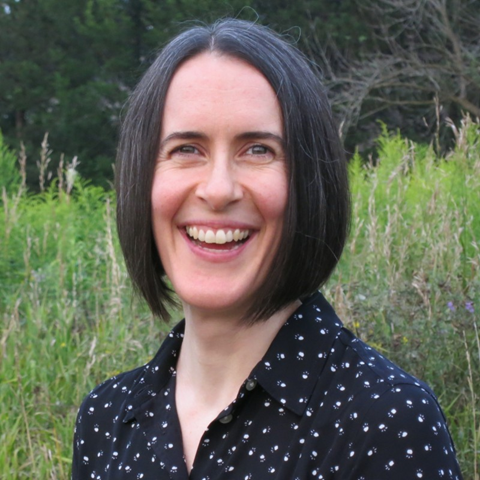
\includegraphics[width=0.25\textwidth]{Other_Figures/FColl.png} 
\end{tabular}		& 		
& \begin{tabular}[c]{@{}c@{}}
\textcolor{white}{Linux}\\
%\textcolor{white}{Linux}\\
\textbf{\underline{Prof. Fiona Coll}}\\
\textbf{Graduate Centre for Academic Communication,}\\ \textbf{University of Toronto}\\
Panelist\\\\
%\vspace{0.2cm}
\begin{tabularx}{\linewidth}{@{}XXX@{}}
Dr. Fiona Coll is an Assistant Professor, Teaching Stream at the Graduate Centre for Academic Communication, and Institute for Studies in Transdisciplinary Engineering Education \& Practice. Her research interests include nineteenth-century conceptions of the relationship between technology and creativity, the efficacy of collaborative writing processes in the classroom, and the role that effect plays in teaching and learning experiences.\\
\qquad Dr. Coll’s work has appeared in numerous journals, including Scholarly Editing, Interdisciplinary Digital Engagement in Arts \& Humanities, and Victorian Review. She is currently co-editing a book collection called Writing Together: Building Social Writing Opportunities for Graduate Students.\\
\qquad At the Graduate Centre for Academic Communication, Dr. Coll leads workshops about graduate-level writing processes and courses on Writing NSERC Proposals and Thesis-Writing in the Physical and Life Sciences.\\
%\textcolor{white}{Linux}\\
\textcolor{white}{Linux}
\end{tabularx}
\end{tabular}\\
\bottomrule
\end{tabular}

\begin{tabular}{  m{0.2\textwidth}  m{0.05\textwidth}  m{0.65\textwidth}  }
\toprule
\begin{tabular}[c]{@{}c@{}} 
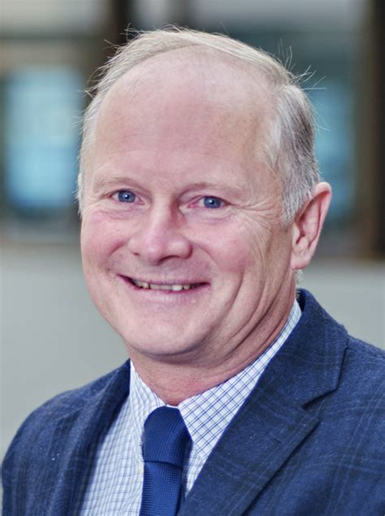
\includegraphics[width=0.25\textwidth]{Other_Figures/DMill.png} 
\end{tabular}		& 		
& \begin{tabular}[c]{@{}c@{}}
\textcolor{white}{Linux}\\
%\textcolor{white}{Linux}\\
\textbf{\underline{Professor R.J. Dwayne Miller}}\\
\textbf{Department of Chemistry, University of Toronto}\\
Panelist\\\\
%\vspace{0.2cm}
\begin{tabularx}{\linewidth}{@{}XXX@{}}
Dr. Dwayne Miller is a professor of Chemistry and Physics at the University of Toronto. His group is engaged in a broad range of research topics that are interrelated by the overarching goal of resolving structure-function relationship of biological systems. Over the years, the Miller group has developed a variety of different technologies, including new laser technology to access different wavelength and temporal regimes.\\
\qquad Dr. Miller has received numerous awards and has made seminal contributions to the development of coherent multidimensional spectroscopy methods and associated ultra-fast laser technology, most notably pioneering the development of ultra-bright electron sources to probe structural dynamics. In 1994, he discovered the mechanism in which proteins are able to find their most optimal equilibrium structure, which has been dubbed ``Collective Mode Coupling''.\\
\qquad Science Rendezvous, an annual event that brings science out of the lab across many Canadian cities, was founded by Dr. Miller in 2008, with the goal of improving student enrollment and public engagement in and with science. In the years since, the committee has had over 300 events with an incredible impact at making science accessible to the general public.\\
%\textcolor{white}{Linux}\\
\textcolor{white}{Linux}
\end{tabularx}
\end{tabular}\\
\midrule
\begin{tabular}[c]{@{}c@{}} 
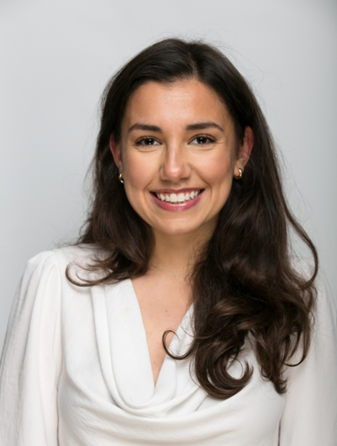
\includegraphics[width=0.25\textwidth]{Other_Figures/MMede.png} 
\end{tabular}		& 		
& \begin{tabular}[c]{@{}c@{}}
\textcolor{white}{Linux}\\
%\textcolor{white}{Linux}\\
\textbf{\underline{Maria Medeleanu}}\\
\textbf{Toronto Science Policy Network}\\ 
\textbf{Department of Physiology, University of Toronto}\\
Panelist\\\\
%\vspace{0.2cm}
\begin{tabularx}{\linewidth}{@{}XXX@{}}
Maria is a PhD Candidate at the Department of Physiology studying how early-life exposures affect immune development and pediatric asthma, and is pursuing a specialization in Public Health Policy at the Dalla Lana School of Public Health. Maria is also Marketing Director for the Toronto Science Policy Network, a student-run science policy group helping scientists at all levels to learn more about and engage in science policy.\\
%\textcolor{white}{Linux}\\
\textcolor{white}{Linux}
\end{tabularx}
\end{tabular}\\
\bottomrule
\end{tabular}

\textcolor{white}{Linux}\\
\textcolor{white}{Linux}\\
\textcolor{white}{Linux}\\
\textcolor{white}{Linux}\\\textcolor{white}{Linux}\\
\textcolor{white}{Linux}\\\textcolor{white}{Linux}\\
\textcolor{white}{Linux}\\\textcolor{white}{Linux}\\
\textcolor{white}{Linux}\\\textcolor{white}{Linux}\\
\textcolor{white}{Linux}\\


%~~~~~~~~~~~~~~~~~~~~~~~~~~~~~~~~~~~~~~~~~~~~~~~~~~~~~~~~~~~~~~~~~~~~
%====================================================================
%~~~~~~~~~~~~~~~~~~~~~~~~~~~~~~~~~~~~~~~~~~~~~~~~~~~~~~~~~~~~~~~~~~~~

% TODO: abstracts, are there any ways to auto newpage without cutting off abstracts?

\chapter*{Abstracts:\\ \textit{Oral Presentations}}
\label{chapter:abstracts_oral}
\markboth{Abstracts: Oral Presentations}{}
\phantomsection\addcontentsline{toc}{chapter}{\hyperref[chapter:abstracts_oral]{Abstracts: Oral Presentations}}

\newpage

\section*{Session I}
\label{sec:sessI}
\phantomsection\addcontentsline{toc}{section}{\hyperref[sec:sessI]{\textbf{Session I: Friday, Apr 28, 3:50 PM}}}

\vspace{0.5cm}

\begin{shaded}
\noindent\textbf{KEYNOTE} \hfill \textbf{\underline{Session I, Fri 3:50 PM}}

\begin{oralabskeynote}
	{Hierarchical functional surfaces for biological sensing and pathogen repellency}
	{Leyla Soleymani}
	{McMaster University}
	In this talk, I will discuss the development of functional hierarchical surfaces for use 
	in biological sensing and biointerfaces. In the area of biological sensing, I will 
	discuss the integration of hierarchical electrodes with functional nucleic acids such 
	as DNA aptamers and DNAzymes for developing tools for the rapid diagnosis of 
	infectious diseases. I will also talk about the pre-clinical validation of these 
	biological sensors and the steps we are taking towards commercialization.\\
	In the area of biointerfaces, I will discuss the engineering of hierarchically-
	structured surfaces for repelling infectious pathogens. More specifically, I will 
	discuss the correlation between structural hierarchy and pathogen repellency. I will 
	talk about the application of these surfaces for repelling both viruses and bacteria 
	and the steps we have taken towards evaluating these surfaces for real-life 
	applications.\\
	Finally, I will discuss the integration of functional repellent surfaces into biological 
	sensors for repelling unwanted interfering agents and detecting the desired target 
	analytes.
	\label{SoleymaniL}
\end{oralabskeynote}
\end{shaded}
\phantomsection\addcontentsline{toc}{subsection}{\hyperref[SoleymaniL]{\textbf{Keynote -- \underline{Leyla Soleymani}}\\Hierarchical functional surfaces for biological sensing and pathogen repellency}}

\vspace{1cm}

\begin{oralabs}
    {Investigating Acyl Carrier Protein Shuttling Pathway in Fungal Fatty Acid Synthase}
    {Elnaz Khalili Samani,$^{1}$ Jennifer W. Lou,$^{1}$ Mohammad Mazhab-jafari,$^{1,2}$}
    {
    $^1$Department of Medical Biophysics, University of Toronto\\
    $^2$Princess Margaret Cancer Research Tower, University Health Network
    }
    {Session I, Fri 4:50 PM}
    Fungal Fatty Acid Synthase (FAS) is a well-structured and highly stable complex that is responsible for de novo fatty acid biosynthesis, with approximately 95\% of the assembly being static. It was found that `six' copies of each FAS1 and FAS2 gene product, termed $\beta$- and $\alpha$-chains, respectively, form a 2.7 MDa barrel-shaped complex intersected at the equator with a central disk, creating `two' reaction chambers. Each chamber contains `three sets' of all catalytic domains for fatty acid synthesis. The mobile acyl-carrier protein (ACP) domain is responsible for shuttling covalently attached substrates and intermediates to six different catalytic sites. The `three-fold symmetry' of the reaction chamber in FAS and the long, flexible linkers tethering ACP domains grant one ACP domain access to three of `each' catalytic center. However, the substrate shuttling pathway of one ACP remains elusive, as it is not possible to align ACP flexible linkers in cryo-EM image processing. Here, for the first time, by breaking the symmetry of fungal FAS, we were able to track a single ACP domain in FAS after performing symmetry expansion, signal subtraction, and focused classification on different cryo-EM datasets. Identifying substrate shuttling pathways `between' catalytic centers will provide a mechanistic understanding of fungal FAS function and an insight into the underlying principles of FAS inhibition and activation.
    \label{Khalili samaniE}
\end{oralabs}
\phantomsection\addcontentsline{toc}{subsection}{\hyperref[Khalili samaniE]{\textbf{Elnaz Khalili Samani}\\Investigating Acyl Carrier Protein Shuttling Pathway in Fungal Fatty Acid Synthase}}

\newpage

\begin{oralabs}
	{Microfluidic Spheroid-on-a-chip model for screening of liposome internalization in solid tumors}
	{Ilya Yakavets,$^{1}$ Monica Ayachit,$^{1,2}$ Sina Kheiri,$^{3}$ Faeze Rakhshani,$^{1}$ Samantha Mcwhirter,$^{1}$ Gilbert C. Walker,$^{1}$ Edmond W.k. Young,$^{3,4}$ Eugenia Kumacheva,$^{1,4,5}$}
	{
	$^1$Department of Chemistry, University of Toronto\\
	$^2$Department of Chemistry, Queen's University\\
	$^3$Department of Mechanical \& Industrial Engineering, University of Toronto\\
	$^4$Institute of Biomedical Engineering, University of Toronto\\
	$^5$Department of Chemical Engineering and Applied Chemistry, University of Toronto
	}
	{Session I, Fri 5:10 PM}
	Nanomedicine has the potential to improve the biodistribution of encapsulated compounds by delivering them selectively to the pathological site and/or avoiding exposure of potentially endangered tissues (site-avoidance drug delivery). To improve the prediction of the performance of nanoparticles (NPs) within the human body, the development of preclinical in vitro tumor models to represent the complex processes of NPs transport under close-to-physiological flow is of great importance. In the present work, we developed an innovative MF spheroid-on-a-chip platform utilizing a biomimetic hydrogel matrix, uniformly sized spheroids, and spheroid growth under near physiological flow. To study the size-dependent penetration of liposomes in the microgels and in the breast cancer spheroids, fluorescently-labelled liposomes with different dimensions were generated by employing microfluidic (MF) hydrodynamic focusing method and supplied to cell-free microgels and breast cancer spheroids in a MF spheroid-on-a-chip platform. We explored the effect of bidirectional flow on accumulation of liposomes with hydrodynamic diameters from 40 to 200~nm in cell-free biomimetic microgels. Following the study of liposomes transport in microgels, we demonstrated the size-dependent accumulation, retention and penetration of liposomes in MCF-7 breast cancer spheroids under near-to-physiological flow. Given the versatility of the MF platform in growing various tissues, it can be used for the screening of nanomaterials for a wide range of applications, including cosmetics and vaccine development.
	\label{YakavetsI}
\end{oralabs}
\phantomsection\addcontentsline{toc}{subsection}{\hyperref[YakavetsI]{\textbf{Ilya Yakavets}\\Microfluidic Spheroid-on-a-chip model for screening of liposome internalization in solid tumors}}

\vspace{1cm}

\begin{oralabswfig}
	{A new role for the proton motive force in bacterial efflux pumps}
	{Duncan Kirby,$^{1}$ Matthew Gerry,$^{1}$ Anton Zilman,$^{1}$}
	{
	$^1$Department of Physics, University of Toronto
	}
	{Session I, Fri 5:30 PM}
	{abstract_figures/Gerry_Matthew_Oral.png}
	{7.0}
	{5.0}
	Efflux pumps on the cell membrane offer an important mechanism by which bacteria become resistant to antibiotics, posing serious problems for public health. These pumps are known to have broad specificity, undermining the efficacy of a wide range of drugs and limiting options for treatment. I will discuss ongoing work towards a quantitative characterization of efflux pump kinetics, particularly the factors giving rise to their broad specificity. Motivated by experimentally determined information about their structure and kinetics, we model the operation of efflux pumps a Markov jump process between various states associated with different conformations and bound ligands. Tuning the parameters of this model has shown that the specificity is determined not only by the drug binding affinity to the pump, but also the periplasmic proton concentration and the periplasmic membrane potential. This offers new insight into the possible origins of broad specificity in hopes of assisting in the development of treatments that will overcome antibiotic resistance. In addition to these main results, I will summarize efforts we are taking to introduce greater complexity to the model and investigate the corresponding effects on efflux pump operation.
	\label{GerryM}
\end{oralabswfig}
\phantomsection\addcontentsline{toc}{subsection}{\hyperref[GerryM]{\textbf{Matthew Gerry}\\A new role for the proton motive force in bacterial efflux pumps}}

\newpage

\section*{Session II}
\label{sec:sessII}
\phantomsection\addcontentsline{toc}{section}{\hyperref[sec:sessII]{\textbf{Session II: Saturday, Apr 29, 9:00 AM}}}

\vspace{0.5cm}

\begin{shaded}
\noindent\textbf{KEYNOTE} \hfill \textbf{\underline{Session I, Fri 3:50 PM}}

\begin{oralabskeynote}
	{Chaperoning Unfolded Outer Membrane Proteins}
	{Karen Fleming}
	{Johns Hopkins University}
	The periplasmic chaperone network ensures the biogenesis of bacterial outer membrane proteins 
	(OMPs). Because the periplasm is devoid of external energy (e.g. ATP), this chaperone network 
	relies only on the thermodynamics and kinetics of binding to unfolded OMPs to maintain these 
	clients in unfolded but folding-competent conformations. We use a combination of solution 
	biophysics, binding, hydrodynamics, scattering analysis, computational flux modeling and 
	integrative structural modeling to investigate how the three main soluble chaperones accomplish 
	their function. Our results show that distinct members of the uOMP conformational ensemble are
	recognized by different chaperones. Skp captures the majority compact forms of the intrinsic 
	uOMP ensemble whereas SurA recognizes the more expanded but rarer expanded forms. These 
	structural differences highlight the different functions of the chaperone network.
	\label{FlemingK}
\end{oralabskeynote}
\end{shaded}
\phantomsection\addcontentsline{toc}{subsection}{\hyperref[FlemingK]{\textbf{Keynote -- \underline{Karen Fleming}}\\Chaperoning Unfolded Outer Membrane Proteins}}

\vspace{1cm}

\begin{oralabs}
    {Flexible client-dependent cages in the assembly landscape of the periplasmic protease-chaperone DegP}
    {Robert W. Harkness,$^{1}$ Zev A. Ripstein,$^{2}$ Justin M. Di Trani,$^{2}$ Lewis E. Kay,$^{1}$}
    {
    $^1$University of Toronto, Department of Molecular Genetics\\
    $^2$SickKids Research Institute, Program in Molecular Medicine
    }
    {Session II, Sat 10:00 AM}
    The periplasmic protein DegP, that is implicated in virulence factor transport leading to pathogenicity, is a bi-functional protease and chaperone that maintains protein homeostasis in gram-negative bacteria. To perform these functions, DegP captures clients inside cage-like structures, which we have recently shown to form through the reorganization of high-order preformed apo-oligomers, consisting of trimeric building blocks, that are structurally distinct from client-bound cages. Our previous studies suggested that these apo oligomers may allow DegP to encapsulate clients of various sizes under protein folding stresses by forming cage ensembles that can include extremely large cage particles, but how this occurs remains an open question. To explore the relation between cage and substrate sizes, we engineered a series of DegP clients of increasing hydrodynamic radii and analyzed their influence on DegP cage formation. We used dynamic light scattering and cryogenic electron microscopy to characterize the hydrodynamic properties and structures of the DegP cages that are adopted in response to each client. We present a series of flexible cage structures including novel 30mer and 60mer particles. Key interactions between DegP trimers and the bound clients that stabilize the cage assemblies and prime the clients for catalysis are revealed. We also provide evidence that DegP can form cages which approach subcellular organelles in terms of size.
    \label{HarknessR}
\end{oralabs}
\phantomsection\addcontentsline{toc}{subsection}{\hyperref[HarknessR]{\textbf{Rob Harkness}\\Flexible client-dependent cages in the assembly landscape of the periplasmic protease-chaperone DegP}}

\newpage

\begin{oralabswref}
	{Promoting single-file capture by pulley effect}
	{Navid Afrasiabian,$^{1}$ Matthew Wei,$^{1}$ Colin Denniston,$^{1}$}
	{
	$^1$Department of Physics and Astronomy, University of Western Ontario, London, Canada
	}
	{Session II, Sat 10:20 AM}
	{
	{[1]} Afrasiabian, N., \& Denniston, C. (2020). The journey of a single polymer chain to a nanopore. Soft Matter, 16(39), 9101-9112.
	}
	Solid-state nanopore sensors remain a promising solution to the rising global demand for genome sequencing. One of the challenges in single-molecule sequencing is threading of folded conformations called hairpins. In a previous publication, we discovered a hairpin unravelling mechanism, namely the pulley effect, in a pressure-driven polymer translocation. In this work, we further investigate the pulley effect in a hydrodynamically driven system and in the presence of electric fields as a method of increasing the single-file capture rate.
	\label{AfrasiabianN}
\end{oralabswref}
\phantomsection\addcontentsline{toc}{subsection}{\hyperref[AfrasiabianN]{\textbf{Navid Afrasiabian}\\Promoting single-file capture by pulley effect}}

\vspace{1cm}

\begin{oralabs}
    {Modelling diffusive protein target search in endoplasmic reticulum tubes}
    {Junyeong Kim,$^{1}$ Aidan Brown,$^{1}$}
    {
    $^1$Department of Physics, Toronto Metropolitan University\\
    }
    {Session II, Sat 10:40 AM}
    The endoplasmic reticulum (ER) is a network of sheet-like and tubular structures that spans much of the cell. Proteins in the ER undergo diffusive searches for various targets, such as unfolded proteins finding chaperones to assist folding or receptors to initiate the unfolded protein response, and folded proteins finding exit sites for export from the ER. Our goal is to describe how ER tube geometry controls diffusive target search. We apply a Brownian Dynamics algorithm to simulate protein diffusion in a cylindrical tube until a target on the tube wall is encountered or the protein escapes the tube. We determine the probability that the protein will encounter the target and the time required to find the target as the tube radius and length, as well as the target size, are varied. We find that targets are more likely to be found for longer and narrower tubes, and larger targets. As ER proteins are in both the ER membrane and lumen, we explore differences in the diffusive search between the tube surface and interior volume, and find that search in the tube volume is substantially more sensitive to the tube geometry compared to search on the tube surface. Our results suggest that, for low-density targets, both ER membrane and lumen proteins are very likely to encounter a nearby target before diffusing to the vicinity of another target.
    \label{KimJ}
\end{oralabs}
\phantomsection\addcontentsline{toc}{subsection}{\hyperref[KimJ]{\textbf{Junyeong Kim}\\Modelling diffusive protein target search in endoplasmic reticulum tubes}}

\newpage

\section*{Session III}
\label{sec:sessIII}
\phantomsection\addcontentsline{toc}{section}{\hyperref[sec:sessIII]{\textbf{Session III: Saturday, Apr 29, 11:15 AM}}}

\vspace{0.5cm}

\begin{shaded}
\noindent\textbf{KEYNOTE} \hfill \textbf{\underline{Session III, Sat 11:15 AM}}

\begin{oralabskeynote}
	{mRNAs control the conformations of proteins with disordered regions}
	{Christine Mayr}
	{Sloan Kettering Institute}
	Two thirds of human proteins have folded domains and intrinsically disordered regions (IDRs). 
	Whereas protein complex assembly involving folded domains has been studied extensively, the 
	rules that govern protein complex assembly involving IDRs are poorly understood. As IDRs are 
	enriched in regulatory factors, including transcription factors and enzymes, it is important to 
	understand how proteins with IDRs – which often have many different binding partners – 
	regulate protein complex assembly. \\
	We recently discovered that protein complexes that involve IDRs are established in an mRNA-
	dependent manner during translation in cytoplasmic condensates, such as TIS granules. Some 
	TIS granule-enriched mRNAs have features that allow them to bind to the IDRs during 
	translation, change their conformational ensembles, and enable specific protein interactors to 
	bind. Because of these features, we call these mRNAs IDR chaperones. Intriguingly, as IDR 
	chaperones are not present in sufficient concentration in the cytosol, translation of the IDRs in 
	the cytosol does not promote co-translational protein complex assembly. \\
	Taken together, we found that mRNA is an important regulator of protein complex assembly 
	involving IDRs. We envision that engineered RNA may be used in the future to control protein 
	activity.
	\label{MayrC}
\end{oralabskeynote}
\end{shaded}
\phantomsection\addcontentsline{toc}{subsection}{\hyperref[MayrC]{\textbf{Keynote -- \underline{Christine Mayr}}\\mRNAs control the conformations of proteins with disordered regions}}

\vspace{1cm}

\begin{oralabs}
	{Mechanism of Calcium Sensitivity Modulation of Cardiac Troponin C by Small Molecules Illuminated by Umbrella Sampling Simulations}
	{Steffen Lindert,$^{1}$}
	{
	$^1$Department of Chemistry and Biochemistry, Ohio State University
	}
	{Session III, Sat 12:15 PM}
	Cardiac troponin C (cTnC) binds intracellular calcium and subsequently cardiac troponin I (cTnI), initiating cardiac muscle contraction. Due to its role in contraction, cTnC has been a therapeutic target in the search for small molecules to treat cardiomyopathies that interfere with normal muscle contraction. Structural studies have shown the binding location of small molecules such as bepridil, dfbp-o, 3-methyldiphenylamine (DPA) and W7 to be a hydrophobic pocket in the regulatory domain of cTnC (cNTnC) but have not shown the influence of these small molecules on the dynamics of opening this domain. Here we describe an application of an umbrella sampling method used to elucidate the impact these calcium sensitivity modulators have on the free energy of cNTnC hydrophobic patch opening. We found that all these molecules lowered the free energy of opening in the absence of the cTnI, with bepridil facilitating the least endergonic transformation. In the presence of cTnI, however, we saw a stabilization of the open configuration due to DPA and dfbp-o binding, and a destabilization of the open configuration imparted by bepridil and W7. Predicted poor binding molecule NSC34337 left the hydrophobic immediately in conventional MD simulations suggesting that only hydrophobic patch binders stabilized the open conformation. Additionally, differences in the free energy of hydrophobic patch opening of hypertrophic (HCM) and dilated cardiomyopathy (DCM) cTnC systems were investigated. Molecular dynamics and umbrella sampling simulations revealed a lower free energy of opening for the HCM mutations A8V and A31S, as well as the calcium-sensitizing mutation L48Q. The DCM mutations, Y5H, Q50R, and E59D/D75Y, all exhibited a higher free energy of opening. In conclusion, our developed simulation protocol presents a novel approach to study calcium sensitivity modulation by small molecules and mutations and facilitates a molecular understanding of cardiac muscle contraction.
	\label{LindertS}
\end{oralabs}
\phantomsection\addcontentsline{toc}{subsection}{\hyperref[LindertS]{\textbf{Steffen Lindert}\\Mechanism of Calcium Sensitivity Modulation of Cardiac Troponin C by Small Molecules Illuminated by Umbrella Sampling Simulations}}

\vspace{1cm}

\begin{oralabswrefwfig}
    {Elucidating inclusion body structure formed by an $\alpha$-helix protein}
    {Bruna Siebeneichler,$^{1}$ Aastha Gandhi,$^{1}$ Elizabeth Meiering,$^{1}$}
    {
    $^1$Department of Chemistry, University of Waterloo, Ontario, Canada
    }
    {Session III, Sat 12:35 PM}
    {
    {[1]} C\'{e}spedes, M. V., Cano-Garrido, O., Álamo, P., Sala, R., Gallardo, A., Serna, N., Falgàs, A., Voltà-Durán, E., Casanova, I., Sánchez-Chardi, A., López-Laguna, H., Sánchez-García, L., Sánchez, J. M., Unzueta, U., Vázquez, E., Mangues, R., \& Villaverde, A. (2020). Engineering Secretory Amyloids for Remote and Highly Selective Destruction of Metastatic Foci. \emph{Advanced Materials}, \emph{32}(7), 1--9. https://doi.org/10.1002/adma.201907348\\
    {[2]} Naser, D., Tarasca, M. V, Siebeneichler, B., Schaefer, A., Deol, H. K., Soule, T. G. B., Almey, J., Kelso, S., Mishra, G. G., Simon, H., \& Meiering, E. M. (2022). High‐Resolution NMR H/D Exchange of Human Superoxide Dismutase Inclusion Bodies Reveals Significant Native Features Despite Structural Heterogeneity. \emph{Angewandte Chemie}, \emph{134}(24). https://doi.org/10.1002/ange.202112645\\
    {[3]} Schaefer, A., Naser, D., Siebeneichler, B., Tarasca, M. V., \& Meiering, E. M. (2022). Methodological advances and strategies for high resolution structure determination of cellular protein aggregates. \emph{Journal of Biological Chemistry}, \emph{298}(9), 102197. https://doi.org/10.1016/j.jbc.2022.102197
    }
    {abstract_figures/Siebeneichler_Bruna_Oral.jpg}
    {11.0}
    {5.0}
    Inclusion bodies (IBs) are nanoparticles consisting of self-assembling proteins that have emerged as promising functional vehicles due to their biocompatibility, biodegradability, and functional versatility (1). Their applicability ranges from biomedicine as an intracellular delivery system to industry as immobilized enzymes. Previously, studies reported $\beta$-sheet proteins forming IB with native-like and amyloid structures (\emph{2}). Here, we investigated IBs formed by an $\alpha$-helical protein model, sperm whale apomyoglobin (apoMb). ApoMb folding is studied through three N-terminal fragments of increasing length: apoMb 77, apoMb 119, and full-length apoMb WT. A powerful set of complementary methods were used to elucidate the apoMb IB structure. The chemical denaturation and washing are able to reveal the global stability. Fourier-transform infrared spectroscopy (FTIR) can determine secondary structure. Lastly, quenched amide hydrogen-deuterium exchange (qHDX) monitored by nuclear magnetic resonance (NMR) is used to inform residue-specific structure information (\emph{3}). The apoMb 77 fragment demonstrated more $\beta$-sheet structure by FTIR and also more chemical stability indicating possible presence of other aggregates such amyloid. The protection pattern for all the constructs showed similar protection in the first 77 residues. Interestingly, there is a higher protection in the regions corresponding to the first $\alpha$-helix in the sequence that accordingly to some in vitro studies is evolved in the formation of the final structure. Moreover, this region is not prone to aggregate based on ZipperDB predictor. These results indicate the possibly native-like $\alpha$-helix content in the IB structure. These findings provide fundamental knowledge for the molecular basis of protein aggregation to rational modify the aggregation pathway.
    \label{SiebeneichlerB}
\end{oralabswrefwfig}
\phantomsection\addcontentsline{toc}{subsection}{\hyperref[SiebeneichlerB]{\textbf{Bruna Siebeneichler}\\Elucidating inclusion body structure formed by an $\alpha$-helix protein}}

\newpage

\begin{oralabswrefwfig}
	{Non-bonded parameters for biological force field derived from Atom-in-molecules approaches.}
	{Carlos Castillo Orellana,$^{1,2}$ Esteban V\"{o}hringer-martinez,$^{2}$ Farnaz Heidar-zadeh,$^{1}$}
	{
	$^1$Department of Chemistry, Queen's University\\
	$^2$Departamento de Fisicoquímica, Universidad de Concepción, Chile
	}
	{Session III, Sat 12:55 PM}
	{
	{[1]} Adcock, Stewart A., and J. Andrew McCammon. ``Molecular Dynamics:~ Survey of Methods for Simulating the Activity of Proteins.'' Chemical Reviews, vol. 106, no. 5, May 2006, pp. 1589--615, https://doi.org/10.1021/cr040426m.\\
	{[2]} Harrison, Judith A., et al. ``Review of Force Fields and Intermolecular Potentials Used in Atomistic Computational Materials Research.'' Applied Physics Reviews, vol. 5, no. 3, Sept. 2018, p. 031104, https://doi.org/10.1063/1.5020808.\\
	{[3]} Pujal, Leila, et al. ``Constrained Iterative Hirshfeld Charges: A Variational Approach.'' The Journal of Chemical Physics, Apr. 2022, p. 5.0089466, https://doi.org/10.1063/5.0089466.
	}
	{abstract_figures/Castillo Orellana_Carlos Andres_Oral.png}
	{10.0}
	{4.0}
	Molecular dynamics simulations are very powerful tools to get energetic and structural insights into large biological molecules on an atomistic scale. At the heart of most molecular dynamic simulations, we find the force field, a set of mathematical functions that model the interactions between atoms based on classical physics, which is combined with an integrator to model the evolution of the system over time {[}1{]}. The force field functions require atom-specific parameters to model the interactions of (non-)bonded atoms which are often obtained from empirical or fitting methods. The main shortcoming of this procedure is that the obtained force field is accurate just for the class of systems or the observables for which it was developed {[}2{]}.\\In recent years, there has been renewed interest in obtaining force field parameters from first principles quantum calculations, as they gave promising results to model the interaction of proteins and small molecules. In this work, I present a novel approach to derive non-bonded force-field parameters directly from atoms-in-molecules (AIM) partitioning of molecular quantum calculations {[}3{]}. The specific method I use is based on a variational principle which provides the flexibility to constrain certain parameters which are desired to remain unchanged. This method is applied to a dataset of sidechain-sidechain residues and the parameters obtained are tested to check if the electrostatic and dispersion interactions are well modeled.
	\label{Castillo orellanaC}
\end{oralabswrefwfig}
\phantomsection\addcontentsline{toc}{subsection}{\hyperref[Castillo orellanaC]{\textbf{Carlos Castillo Orellana}\\Non-bonded parameters for biological force field derived from Atom-in-molecules approaches.}}


\newpage

\section*{Session IV}
\label{sec:sessIV}
\phantomsection\addcontentsline{toc}{section}{\hyperref[sec:sessIV]{\textbf{Session IV: Saturday, Apr 29, 4:30 PM}}}

\vspace{0.5cm}

\begin{shaded}
\noindent\textbf{KEYNOTE} \hfill \textbf{\underline{Session IV, Sat 4:30 PM}}

\begin{oralabskeynote}
	{Mapping cell volume and mechanical changes within tumor spheroids under confinement}
	{Anna Taubenberger}
	{TU Dresden}
	Tumor tissues are mechanically altered across multiple spatial scales,
	from the subcellular to the tissue level, and these changes contribute to
	cancer progression. Effects of mechanically altered microenvironments on
	tumor cells are well studied in a systematic manner using bioengineered
	3D in vitro models. Previous studies indicate that tumor spheroids adapt
	their growth and mechanical properties when grown in confining 3D
	microenvironments. Still, the temporal dynamics and molecular basis of
	this mechanical adaption remain poorly understood. Here we cultured
	tumor spheroids grown from single cancer cells in mechanically well-
	defined biohybrid ECM mimicking hydrogels. Growth in stiffened hydrogels
	was associated with changes in cell morphology, gene expression, and
	spheroid growth. Brillouin microscopy in-situ mapping revealed that cells
	tumor spheroids altered their mechanical properties under confinement
	and when acquiring invasive traits. Within few days, transitions from
	single cells to multicellular structures were associated with drastic cell
	volume decreases and higher Brillouin frequency shifts. Drugs interfering
	with cell-cell junctions and intermediate filaments but not F-actin
	filaments nor microtubules affected the mechanical phenotype of cells
	measured by Brillouin microscopy. Taken together, our study provides
	insights into how tumor cells adapt their volumes and mechanical
	properties to microenvironment stiffness and confinement and when
	forming multicellular and invasive structures, which are relevant aspects
	in tumorigenesis and tumor progression.
	\label{TaubenbergerA}
\end{oralabskeynote}
\end{shaded}
\phantomsection\addcontentsline{toc}{subsection}{\hyperref[TaubenbergerA]{\textbf{Keynote -- \underline{Anna Taubenberger}}\\Mapping cell volume and mechanical changes within tumor spheroids under confinement}}

\newpage

\begin{oralabswfig}
	{Protein Dynamics in a Crystal are Functionally Relevant}
	{Eugene Klyshko,$^{1,2}$ Justin Sung-Ho Kim,$^{1,2}$ Lauren Mcgough,$^{3}$ Victoria Valeeva,$^{2}$ Rama Ranganathan,$^{4}$ Sarah Rauscher,$^{1,2,5}$}
	{
	$^1$Department of Physics, University of Toronto, Toronto, ON\\
	$^2$Department of Chemical and Physical Sciences, University of Toronto Mississauga, Mississauga, ON, Canada\\
	$^3$Department of Ecology and Evolution, The University of Chicago, Chicago, IL, USA\\
	$^4$Department of Biology and Molecular Biochemistry, The University of Chicago, Chicago, IL, USA\\
	$^5$Department of Chemistry, University of Toronto, Toronto, ON, Canada
	}
	{Session IV, Sat 5:30 PM}
	{abstract_figures/Rauscher_Sarah_Oral.pdf}
	{6.0}
	{6.0}
	In order to fully understand the function of proteins, it is necessary to have a detailed description of their motions at the atomic level. New ``pump-probe'' methods, such as electric-field and temperature-jump stimulated time-resolved X-ray diffraction, have opened up ways to initiate and observe protein motions with atomistic detail on biologically relevant timescales. However, the ensemble-averaged description of protein motions obtained in these experiments requires the parallel development of effective molecular dynamics (MD) approaches to capture the diverse conformational ensemble of proteins within a crystal. We characterized the equilibrium state of a PDZ domain crystal using MD and addressed the challenges associated with equilibration, modeling of crystal environment, and choice of force fields. We identify critical factors controlling the agreement between the simulations and experiment, establishing that the simulations using the Amber ff14SB force field most accurately reproduce the crystal structure. Using these equilibrium simulations, we found that the structural changes of the protein in the crystal resemble ligand-induced conformational changes in other PDZ domain homologues, which suggests that the motions observed in the crystal are functionally relevant. This work lays the foundations for a virtuous cycle between simulation and the new pump-probe experiments for visualizing and understanding functional motions of proteins.
	\label{RauscherS}
\end{oralabswfig}
\phantomsection\addcontentsline{toc}{subsection}{\hyperref[RauscherS]{\textbf{Sarah Rauscher}\\Protein Dynamics in a Crystal are Functionally Relevant}}

\newpage

\begin{oralabswref}
	{Ultrasound-imaging of Picosecond Infrared Laser Ablation}
	{Manoel L. Da Silva-neto,$^{1}$ Sam Keramati,$^{1}$ Sreelaja P. Vadhyar,$^{1}$ Temitope T. Abiola,$^{1}$ Yohannes Soenjaya,$^{3}$ Samansa Maneshi,$^{1}$ Renzhong Hua,$^{1}$ Christine E. M. Demore,$^{3,4}$ F. Stuart Foster,$^{3,4}$ R. J. Dwayne Milller,$^{1,2}$}
	{
	$^1$Department of Chemistry, University of Toronto, ON, Canada M5S 3H6\\
	$^2$Department of Physics, University of Toronto, ON, Canada M5S 3H6\\
	$^3$Sunnybrook Research Institute, Sunnybrook Health Sciences Center, Toronto, ON, Canada\\
	$^4$Department of Medical Biophysics, University of Toronto, Toronto, ON, Canada
	}
	{Session IV, Sat 5:50 PM}
	{
	{[1]} Cowan, M. L. \emph{et al}., Ultrafast memory loss and energy redistribution in the hydrogen bond network of liquid H\textsubscript{2}O. Nature 2005, 434 (7030), 199-202.\\doi: 10.1038/nature03383\\
	{[2]} Wu, Y. \emph{et al}., Nanodiamond Theranostic for Light-Controlled Intracellular Heating and Nanoscale Temperature Sensing. Nano Lett. 2021, 21, 9, 3780--3788. doi: 10.1021/acs.nanolett.1c00043\\
	{[3]} Zhao, L. \emph{et. al.}, Recent advances in selective photothermal therapy of tumor. J Nanobiotechnology. 2021; 19: 335. doi: 10.1186/s12951-021-01080-3
	}
	Picosecond Infrared Laser (PIRL) developed in our group is specifically engineered to selectively excite the water in tissue to highly localize the energy. Water acts as a propellant to drive biomolecules and proteins within the absorption volume into the gas phase completely intact, faster than nucleation formation, and without cavitation-induced shock waves {[}1{]}.\\Cell death happens at temperatures above 50°C {[}2{]}. The technique of Photothermal Therapy (PTT) is based on this property. PTT is used for treating cancerous tumors, where laser irradiation generates that {[}3{]}. The PTT process is made more efficient by adding Photothermal Agents (PTA's). However, materials such as metallic nanoparticles and organic dyes have several disadvantages such as poor water solubility, limited accumulation inside the tumor, and poor biocompatibility. PIRL is capable of generating the required heat without the use of PTAs. The high degree of absorption of PIRL by water leads to heat generation.\\Currently, focal therapy techniques are employed in the treatment of cancer. To be effective, focal therapy must be guided by imaging to target the desired area and to monitor the untreated areas. Ultrasound imaging is a suitable technique for real-time imaging due to its low cost, high image quality, and small form factor. Here, we employ ultrasound imaging to guide the PIRL ablation in real-time in phantoms and tissues and to image the tissue disruption. The use of Ultrasound imaging to guide the optical fiber that carries the PIRL beam to the desired areas inside tissue will also be demonstrated.
	\label{Da silva netoM}
\end{oralabswref}
\phantomsection\addcontentsline{toc}{subsection}{\hyperref[Da silva netoM]{\textbf{Manoel Leonardo da Silva-Neto}\\Ultrasound-imaging of Picosecond Infrared Laser Ablation}}

\newpage

\begin{oralabs}
    {TOC159 Receptors are Anchored in the Chloroplast Outer Envelope by a $\beta$-Barrel and Targeted Using a Bi-Partite Signal at the C-Terminus}
    {Michael Fish,$^{1}$ Simon Chuong,$^{2}$ Masoud Jelokhani-niaraki,$^{3}$ Matthew Smith,$^{1}$}
    {
    $^1$Department of Biology, Wilfrid Laurier University\\
    $^2$Department of Biology, University of Waterloo\\
    $^3$Department of Chemistry \& Biochemistry, Wilfrid Laurier University
    }
    {Session IV, Sat 6:10 PM}
    TOC159 receptors are an important group of outer envelope proteins of the chloroplast and key component of the translocation machinery (TOC complex), together with TOC34 receptors and the TOC75 translocation channel, which recognize N-terminal chloroplast transit peptides and import chloroplast preproteins from the cytosol. The structure and targeting pathway of TOC34 and TOC75 are well characterized, but the same for TOC159 receptors has proven difficult to describe. Using circular dichroism spectroscopy, we show that TOC159 receptor homologs expressed in \emph{Escherichia coli} and purified from inclusion bodies form $\beta$-barrel structures in detergent and when reconstituted in lipid bilayers, like TOC75. Further, we use GFP fusion protein targeting assays in plant cells to demonstrate that TOC159 receptors use a bi-partite targeting signal at their C-terminus to reach the chloroplast outer envelope. The targeting signal is composed of a highly conserved $\beta$-signal, like those found in $\beta$-barrel proteins of mitochondria and gram-negative bacteria. The second component of the targeting signal is a reverse transit peptide-like sequence which may have evolved to preclude mitochondrial targeting in the unique cellular environmental of algae and plants, which house plastids and mitochondria, endosymbiotic organelles that both contain outer membrane $\beta$-barrels. Characterizing how TOC159 receptors are targeted to and anchored in the chloroplast outer envelope will lead to a better understanding of their role in the assembly of functionally diverse TOC complexes responsible for regulating chloroplast biogenesis and plastid transitions in plant cells.
    \label{FishM}
\end{oralabs}
\phantomsection\addcontentsline{toc}{subsection}{\hyperref[FishM]{\textbf{Michael Fish}\\TOC159 Receptors are Anchored in the Chloroplast Outer Envelope by a $\beta$-Barrel and Targeted Using a Bi-Partite Signal at the C-Terminus}}

\newpage

\section*{Session V}
\label{sec:sessV}
\phantomsection\addcontentsline{toc}{section}{\hyperref[sec:sessV]{\textbf{Session V: Sunday, Apr 30, 9:00 AM}}}

\vspace{0.5cm}

\begin{shaded}
\noindent\textbf{KEYNOTE} \hfill \textbf{\underline{Session V, Sun 9:00 AM}}

\begin{oralabswfigkeynote}
	{Transforming nature's switches into our biotech tools and therapeutics}
	{Kevin Gardner}
	{City College of New York}
	{abstract_figures/Gardner_Kevin.png}
	{10.0}
	{5.0}
	Environmental cues regulate many biological processes, coordinating cellular pathways 
	to respond to changing conditions.  Such regulation is often initiated by sensory protein 
	domains which expand their chemical repertoire by using small molecule ligands to 
	convert environmentally-triggered changes into altered protein/protein interactions.  
	Using a combination of biophysics, biochemistry and synthetic chemistry, we study the 
	mechanistic controls of such domains for both fundamental understanding and 
	subsequent artificial control.  Here I will discuss two examples of this principle, showing 
	how such signaling proteins can be converted into novel biotech tools or targeted by 
	small molecule therapeutics, including Merck's newly-approved belzutifan, a first in-class
	anti-cancer therapeutic targeting the Hypoxia Inducible Factor 2 (HIF-2) transcription 
	factor.  Future directions stemming from this work will also be discussed.
	\label{GardnerK}
\end{oralabswfigkeynote}
\end{shaded}
\phantomsection\addcontentsline{toc}{subsection}{\hyperref[GardnerK]{\textbf{Keynote -- \underline{Kevin Gardner}}\\Transforming nature's switches into our biotech tools and therapeutics}}

\vspace{1cm}

\begin{oralabs}
    {Illuminating disorder and dynamics in proteins with single-molecule tools}
    {Claudiu Gradinaru$^{1}$}
    {
    $^1$Department of Chemical and Physical Sciences, UTM
    }
    {Session V, Sat 10:00 AM}
	Proteins are the building blocks of life, and their chemical repertoire drives most biological processes. Some proteins have stable structure but others, called intrinsically disordered proteins (IDPs), are highly flexible. They often function as protein interaction hubs and are involved in many neurodegenerative diseases. Much less disordered than IDPs, yet highly dynamic, G protein-coupled receptors (GPCRs) trigger highly specific cellular responses to subtle environmental clues. They are the major target of pharmaceutical drugs.\\
	In my lab, we capture the molecular choreography of proteins at the single-molecule level. By their very nature, single-molecule methods remove the averaging present other experiments and can reveal rare, possibly pathological states. Using a versatile home-built suite of single-molecule fluorescence microscopes, we can measure distances on the molecular scale, track individual proteins diffusing in the membrane of live cells, count units in a supramolecular complex, and resolve conformational dynamics from nanosecond to second timescales.\\
	In my talk, I will illustrate the power of the single-molecule approach to decode the structure and dynamics of IDPs and GPCRs, using our recent results on two representative cases from each category: the disordered 4E-BP2 protein and the adenosine $\mathrm{A_{2A}}$ receptor.
	\label{GradinaruC}
\end{oralabs}
\phantomsection\addcontentsline{toc}{subsection}{\hyperref[GradinaruC]{\textbf{Claudiu Gradinaru}\\Illuminating disorder and dynamics in proteins with single-molecule tools}}

\newpage

\begin{oralabs}
    {Ion permeation mechanism of Cystic Fibrosis Transmembrane Conductance Regulator (CFTR)}
    {Zhi-Wei Zeng,$^{1,2}$ R\'{e}gis Pom\`{e}s,$^{1,2}$}
    {
    $^1$Department of Biochemistry, University of Toronto\\
    $^2$Molecular Medicine, Hospital for Sick Children, Toronto, ON, Canada
    }
    {Session V, Sat 10:20 AM}
    Cystic fibrosis transmembrane conductance regulator (CFTR) is an anion channel that enables water and ion secretion from epithelial cells. Loss-of-function mutations of CFTR causes Cystic Fibrosis (CF), a lethal human disease that can result in the failure of lungs and other exocrine organs/tissues. Due to its great physiological significance, CFTR is the target of extensive amount of research; however, how do anions permeate through the channel remains elusive despite the availability of near-atomistic cryoEM structures. We report MD simulations of phospholipid bilayer-embedded human CFTR starting from its ATP-bound, NBD-dimerized ``near-open'' state from the PDB, allowing it to relax towards an apparent open state. In the presence of transmembrane voltage, the open state can support permeation of chloride ions. The permeation pathway is lined by functionally important residues. Furthermore, we evaluated the single channel conductance of our open state model computationally and propose a plausible role of pore lining residues in facilitating chloride ion permeation through the narrowest region.
    \label{ZengZ}
\end{oralabs}
\phantomsection\addcontentsline{toc}{subsection}{\hyperref[ZengZ]{\textbf{Zhi-Wei Zeng}\\Ion permeation mechanism of Cystic Fibrosis Transmembrane Conductance Regulator (CFTR)}}

\vspace{1cm}

\begin{oralabs}
    {A systematic strategy to link human genetic variations to drug response}
    {Divya Kriti,$^{1}$ Corey Nislow,$^{2,3}$}
    {
    $^1$Department of Biochemistry and Molecular Biology, University of British Columbia\\
    $^2$Faculty of Pharmaceutical Sciences, University of British Columbia\\
    $^3$Department of Biochemistry and Molecular Biology, University of British Columbia
    }
    {Session V, Sat 10:40 AM}
    \textbf{Introduction:}\\Every individual reacts differently to drugs based on their genetic makeup. To understand the why aspect, we need to assess the underlying genetic variation while prioritizing mutations that affect the phenotype. Thus, we have developed a novel approach called ``Variant Technology (V-Tech)" to comprehensively map all clinically actionable human variants in drug targets.\\\textbf{Objectives:}\\1) Identify genetic differences responsible for variations in drug efficacy and toxicity.\\2) Assess the functional impact (i.e., fitness and drug response) of these clinically actionable variants.\\3) Develop predictive models to evaluate the impact of new variants in patients.\\\textbf{Methods:}\\V-Tech strategy involves: (1) characterization of drug-target pairs, (2) performing massively parallel screens of variants for each pair, and (3) bioinformatically correlating actionable variants with drug resistance/sensitivity.\\\textbf{Results:}\\Dihydrofolate reductase (DHFR), the drug target for Methotrexate was interrogated using V-Tech. A site-saturated library of DHFR was designed consisting of 3553 variants featuring non-synonymous and yeast-specific codons. After cloning into yeast deletion strains, libraries were exposed to varying Methotrexate concentrations. Collected samples have been deep-sequenced to decode variant effects.\\\textbf{Conclusion:}\\Adoption of V-Tech by the medical community will lead to an era where the right treatment is given to the right patient at the right dosages allowing for reduced therapeutic costs and personalized health care.
    \label{KritiD}
\end{oralabs}
\phantomsection\addcontentsline{toc}{subsection}{\hyperref[KritiD]{\textbf{Divya Kriti}\\A systematic strategy to link human genetic variations to drug response}}


\newpage

\section*{Session VI}
\label{sec:sessVI}
\phantomsection\addcontentsline{toc}{section}{\hyperref[sec:sessVI]{\textbf{Session VI: Sunday, Apr 30, 11:20 AM}}}

\vspace{0.5cm}

\begin{shaded}
\noindent\textbf{KEYNOTE} \hfill \textbf{\underline{Session VI, Sun 11:20 AM}}

\begin{oralabskeynote}
	{Genetic code interpretation in mammalian organisms}
	{Haissi Cui}
	{University of Toronto}
	Shared among all life forms is that genetic information is stored as 
	DNA, which is transcribed into mRNA and translated into proteins. During this
	process, aminoacyl-tRNA synthetases catalyze the first step of protein 
	synthesis by physically linking the building blocks of proteins, amino acids, to
	transfer-RNA (tRNA) adapters. These “charged” tRNAs are then used by the 
	ribosome to assemble the linked amino acids into proteins according to the 
	information provided by mRNA. Philosophically, tRNA aminoacylation can 
	therefore be seen as the moment during which the genetic code is 
	interpreted, as nucleotide triplets are assigned to amino acids. \\
	Recently, we have come to appreciate that RNA processes in 
	mammalian cells can be highly localized. However, we still do not know 
	where aminoacylation takes place in mammalian cells and which principles 
	govern the trafficking of aminoacyl-tRNA synthetases, partially because we 
	lack appropriate methods to study this process. My group aims to develop 
	and use chemical tools, genome engineering, and relevant disease models to
	visualize aminoacylation, manipulate RNA and protein localization within 
	mammalian cells, and study the consequences of mutations that cause 
	human diseases. Building on previous work, which suggests the control of 
	aminoacyl-tRNA synthetase localization as an evolutionary drive and a 
	regulator of both translational and moonlighting functions, we use a mix of 
	chemistry, biochemistry, cell biology, and animal models to study RNA 
	processes from molecule to mouse.
	\label{CuiH}
\end{oralabskeynote}
\end{shaded}
\phantomsection\addcontentsline{toc}{subsection}{\hyperref[CuiH]{\textbf{Keynote -- \underline{Haissi Cui}}\\Genetic code interpretation in mammalian organisms}}
	
\newpage

\begin{oralabswfig}
    {Structural Studies Probing the Role of Phosphorylation of the Intrinsically Disordered Regulatory Region of the Yeast Cadmium Factor 1 Protein}
    {Sarah C. Bickers,$^{1,2}$ Sarah E. S. Quail,$^{1,2}$ Agatha Tymczak,$^{2,3}$ Dmitry Pichugin,$^{4}$ Voula Kanelis,$^{1,2,3}$}
    {
    $^1$Department of Chemistry, University of Toronto\\
    $^2$Department of Chemical and Physical Sciences, University of Toronto Mississauga\\
    $^3$Department of Cell and Systems Biology, University of Toronto\\
    $^4$Centre for Magnetic Resonance Research, University of Toronto Mississauga
    }
    {Session VI, Sun 12:20 PM}
    {abstract_figures/Bickers_Sarah_Oral.jpg}
    {10.0}
    {8.0}
    The Yeast cadmium factor 1 protein (Ycf1p) is an ATP Binding Cassette (ABC) membrane protein that transports glutathione conjugated metals from the yeast cytoplasm to the vacuole, thereby detoxifying the yeast cell. Ycf1p contains the core ABC protein structure of two half transporters each containing a transmembrane domain (TMD) and nucleotide binding domain (NBD). These two half transporters are linked via the intrinsically disordered regulatory region (RR) to create the ABC protein core arrangement of TMD1-NBD1-RR-TMD2-NBD2. Binding and hydrolysis of ATP at the NBDs causes formation and dissociation of an NBD heterodimer, enabling substrate transport through the TMDs. Like other ABC proteins, the Ycf1p RR is post-translationally modified via phosphorylation. Sites S903, S908, T911, and S914 have been found to be abundantly phosphorylated in Ycf1p, with S908 and T911 phosphorylation increasing ATP hydrolysis of Ycf1p. Despite the prevalence of ABC protein phosphorylation, the molecular basis by which phosphorylation controls protein function is poorly understood. Current electron cryo-microscopy (cryo-EM) structures of Ycf1p reveal a small segment of the phosphorylated RR contacting NBD1, however most of the RR is unresolved due to the dynamic nature of intrinsically disordered regions. Using nuclear magnetic resonance (NMR) spectroscopy, we identified segments of the RR that have residual structure which are disrupted upon phosphorylation. Further biophysical studies using NMR and fluorescence spectroscopy determined phosphorylation dependent changes in interdomain interactions of the RR with NBD1 and NBD2. Together, the cryo-EM structures and in solution experiments provide a mechanistic model of how RR phosphorylation regulates Ycf1p activity.
    \label{BickersS}
\end{oralabswfig}
\phantomsection\addcontentsline{toc}{subsection}{\hyperref[BickersS]{\textbf{Sarah Bickers}\\Structural Studies Probing the Role of Phosphorylation of the Intrinsically Disordered Regulatory Region of the Yeast Cadmium Factor 1 Protein}}

\newpage

\begin{oralabs}
	{Investigating Isomerization Kinetics of Bioinspired Azobenzene Photoswitches as a Novel Optical Sensor for Oxygen}
	{Coral Hillel,$^{1}$ Sara Rough,$^{2}$ Dr. William Pietro,$^{2}$ Dr. Christopher Barrett,$^{1,3}$ Dr. Ozzy Mermut,$^{1}$}
	{
	$^1$Physics and Astronomy, York University\\
	$^2$Chemistry, York University\\
	$^3$Chemistry, McGill University
	}
	{Session VI, Sun 12:40 PM}
	Hypoxia is a characteristic pathophysiological property of advanced solid tumours which influences aggressiveness and resistance to treatments whose mechanisms rely on the presence of oxygen. Measurement of tumour oxygenation is thus vital for stratifying treatment plans by hypoxic severity and monitoring real-time variations in partial pressure of oxygen (pO\textsubscript{2}) caused by high energy X-ray and other photonic therapies. Azobenzene photoswitches present a novel form of oxygen sensing predicated on their isomerization kinetics. Upon irradiation with light, azobenzenes undergo reversible geometric isomerization between stable \emph{trans} and metastable \emph{cis} isomers. The rate of thermal \emph{cis}-\emph{trans} isomerization is sensitive to the molecular environment, which translates into sensor applications.\\A novel bioinspired photoswitch, FePc(PAP)\textsubscript{2}, was synthesized by coordination of 4-phenylazopyridine (PAP) to iron (II) phthalocyanine (FePc), a model system for heme porphyrin in blood that is capable of binding oxygen. Solutions were purged with argon gas or flowed with oxygen gas to modulate pO\textsubscript{2}. Isomerization kinetics were measured by pump-probe isomerization spectroscopy, wherein photoisomerization was initiated by irradiation with a 365 nm LED, and then recovery of the $\pi$-$\pi^{*}$ absorption band was monitored over time with a spectrophotometer.~\\Under ambient oxygenation in non-polar solvent, the isomerization half-life of PAP was found to be several hours while the isomerization rate of FePc(PAP)\textsubscript{2} was an order of magnitude faster than PAP. In this work, isomerization rates of PAP and FePc(PAP)\textsubscript{2} will be determined as a function of oxygen concentration in a proof-of-principle demonstration of a new optical sensor for evaluating tumour oxygenation.
	\label{HillelC}
\end{oralabs}
\phantomsection\addcontentsline{toc}{subsection}{\hyperref[HillelC]{\textbf{Coral Hillel}\\Investigating Isomerization Kinetics of Bioinspired Azobenzene Photoswitches as a Novel Optical Sensor for Oxygen}}

\vspace{1cm}

\begin{oralabswref}
    {Erythro-PmBs: A selective polymyxin B delivery system using antibody-conjugated hybrid erythrocyte liposomes}
    {Hannah Krivic,$^{1}$ Sebastian Himbert,$^{1}$ Ruthie Sun,$^{1}$ Michal Feigis,$^{1}$ Maikel Rheinstadter,$^{1}$}
    {
    $^1$Department of Physics and Astronomy, McMaster University, Hamilton ON
    }
    {Session VI, Sun 1:00 PM}
    {
    {[1]} Krivić, H., Himbert, S., Sun, R., Feigis, M. and Rheinstädter, M.C., 2022. Erythro-PmBs: A Selective Polymyxin B Delivery System Using Antibody-Conjugated Hybrid Erythrocyte Liposomes.~ \emph{ACS Infectious Diseases}.\\
    {[2]} Krivić, H., Himbert, S. and Rheinst\"{a}dter, M.C., 2022. Perspective on the Application of Erythrocyte Liposome-Based Drug Delivery for Infectious Diseases.~ \emph{Membranes},~ \emph{12}(12), p.1226.
    }
    Due to the growing world-wide antibiotic resistance crisis, many currently existing antibiotics have become ineffective due to bacteria developing resistive mechanisms. There are a limited number of potent antibiotics that are successful at suppressing microbial growth; however, these are often deemed as a last resort due to their toxicity. We developed a novel PmB delivery system constructed by conjugating hybrid erythrocyte liposomes with antibacterial antibodies to combine a high loading efficiency with guided delivery {[}1,2{]}. The retention of PmB is enhanced through incorporation of the negatively charged lipid, DMPS, into the red blood cell's cytoplasmic membrane through electrostatic interactions. Molecular dynamics (MD) simulations reveal an optimal fraction of DMPS in the hybrid erythrocyte membranes that allows for complete anchorage of PmB through insertion of their acyl tail into the hydrophobic membrane core. Anti-\emph{Escherichia coli} antibodies are attached to these hybrid erythrocyte liposomes by inclusion of DSPE-PEG maleimide linkers. We show that these erythro-PmBs have a loading efficiency of $\sim$90\% and are effective in delivering PmB to \emph{E.coli}, with values for the minimum inhibitory concentration (MIC) being comparable to those of free PmB. The MIC values for \emph{Klebsiella aerogenes}, however, significantly increased well beyond the resistant breakpoint, indicating that the inclusion of the anti-\emph{E.coli} antibodies enables the erythro-PmBs to selectively deliver antibiotics to specific targets. MD simulations further suggest a fusion or lipid exchange mechanism between the erythro-PmBs and the outer membrane of \emph{E.coli.}
    \label{KrivicH}
\end{oralabswref}
\phantomsection\addcontentsline{toc}{subsection}{\hyperref[KrivicH]{\textbf{Hannah Krivic}\\Erythro-PmBs: A selective polymyxin B delivery system using antibody-conjugated hybrid erythrocyte liposomes}}




%~~~~~~~~~~~~~~~~~~~~~~~~~~~~~~~~~~~~~~~~~~~~~~~~~~~~~~~~~~~~~~~~~~~~
%====================================================================
%~~~~~~~~~~~~~~~~~~~~~~~~~~~~~~~~~~~~~~~~~~~~~~~~~~~~~~~~~~~~~~~~~~~~

\chapter*{Abstracts:\\ \textit{Poster Presentations}}
\label{chapter:abstracts_poster}
\markboth{Abstracts: Poster Presentations}{}
\phantomsection\addcontentsline{toc}{chapter}{\hyperref[chapter:abstracts_poster]{Abstracts: Poster Presentations}}

\newpage

\section*{Biological sensing, imaging, and analytical techniques}
\label{sec:sens}
\phantomsection\addcontentsline{toc}{section}{\hyperref[sec:sens]{\textbf{Biological sensing, imaging, and analytical techniques}}}


\begin{posterabswrefwfig}
	{A Tellurophene-specific Bioorthogonal Reaction for Protein Conjugation and Proteomics}
	{Yong Jia Bu,$^{1}$ Mark Nitz,$^{1}$}
	{
	$^1$Department of Chemistry, University of Toronto
	}
	{P01}
	{
	{[1]} Bassan, J.; Willis, L. M.; Vellanki, R. N.; Nguyen, A.; Edgar, L. J.; Wouters, B.G.; Nitz, M. TePhe, a Tellurium-containing Phenylalanine Mimic, Allows Monitoring of Protein Synthesis in Vivo with Mass Cytometry. \emph{Proc. Natl. Acad. Sci.,}  \textbf{2019,}  \emph{116,} 8155-8160.\\
	{[2]} Vurgun, N.; Nitz, M. Validation of L-Tellurienylalanine as a Phenylalanine Isostere. \emph{ChemBioChem.,}  \textbf{2019,}  \emph{21,} 1136-1139.\\
	{[3]} Bu, Y.J.; Nitz, M. Incorporation of TePhe into Expressed Proteins is Minimally Perturbing. \emph{ChemBioChem.,}  \textbf{2021,}  \emph{22,} 2449-2456.
	}
	{abstract_figures/Bu_Yong Jia_Poster.jpg}
	{10.0}
	{4.0}
	The study of protein synthesis in response to environmental changes is a key element in understanding biological processes. To track active translation, the Nitz group has developed L-tellurienylalanine (TePhe), a tellurium (Te)-containing analogue of the natural amino acid phenylalanine (Phe)\textsuperscript{1}. TePhe is readily taken up by cells and incorporated into nascent proteins in place of Phe\textsuperscript{2,3}, and demonstrates great utility in measuring global translation rates by mass cytometry, which detects the presence of the Te atom. This technique does not yield information regarding the identities of newly synthesized proteins, however. To bridge this gap, we exploited the unique reactivity of the tellurophene side chain of TePhe for covalent tagging. We have discovered that the tellurophene side chain can be rapidly and quantitatively oxidized using \emph{N}-chlorosuccinimide, generating a reactive intermediate which undergoes {[}4+2{]} cycloaddition with the strained alkyne {[}6.1.0{]}bicyclononyne (2\textsuperscript{nd} order rate constant \textgreater{}100 M-\textsuperscript{1} s-\textsuperscript{1}), and which forms a stable benzo-fused cyclooctane adduct upon Te extrusion. This novel reaction, which we term oxidation-controlled, strain-promoted tellurophene alkyne click (OSTAC), enables rapid, robust, and selective conjugation of affinity tags to TePhe-containing proteins in cell lysates, allowing their enrichment away from the background proteome and further analysis by LC-MS/MS. The activatable nature of OSTAC also renders it compatible with other bioorthogonal reactions, including established CuAAC and SPAAC chemistries, allowing detection of multiple probes in a single sample. We are now actively working on validation and comparison of OSTAC to established methods for interrogation of nascent human proteomes.
	\label{BuY}
\end{posterabswrefwfig}
\phantomsection\addcontentsline{toc}{subsection}{\hyperref[BuY]{\textbf{Yong Jia Bu}\\A Tellurophene-specific Bioorthogonal Reaction for Protein Conjugation and Proteomics}}

\newpage

\begin{posterabs}
	{Structure-Affinity Relationship of the Dopamine-Binding Aptamer with Dopamine Derivatives}
	{Emily Hoi Pui Chao ,$^{1}$ Yunus A. Kaiyum,$^{1}$ Cameron Mackereth,$^{2}$ Philip E. Johnson,$^{1}$}
	{
	$^1$Department of Chemistry, York University, 4700 Keele Street, Toronto, Ontario, Canada M3J 1P3\\
	$^2$Institut Europ\'{e}en de Chimie et Biologie, 2 Rue Robert Escarpit-33607, Pessac, France
	}
	{P02}
	The dopamine binding aptamer, DA-Mut3 has been utilized to investigate the binding relationship of aptamer-dopamine ligand interactions because of its high specificity and selectivity. Dopamine is a neurotransmitter that controls emotion and movements in brains and deficiency of dopamine has been linked to Parkinson disease. It is a small ligand with one amine group attached via an ethyl chain and a catechol structure which is a benzene ring with two hydroxyl side groups.\\A series of ITC binding studies were performed to identify the changes in binding affinity with respect to modifications made to dopamine. The data suggests that the primary amine group was a key factor in the recognition of the ligand for DA-Mut3, as modifications made to this site caused loss of binding. Additionally, the two alcohol groups as well as the aliphatic chain length appear to play a role in the interaction between DA-Mut3 and dopamine. The modifications that do not result in a loss of binding are limited indicating a high specificity of this aptamer for dopamine.\\A series of truncation studies of DA-Mut 3 helps to simplify the NMR data analysis. Interestingly, the removal of several bases at the 5' end of were suspected to be adjacent to the binding site led to an increase in binding strength indicated by lower K\textsubscript{d} values­. The goal of this research aims to gain insight into how dopamine aptamer interacts with its ligand and this could help better designing biosensors.
	\label{ChaoE}
\end{posterabs}
\phantomsection\addcontentsline{toc}{subsection}{\hyperref[ChaoE]{\textbf{Emily Hoi Pui Chao}\\Structure-Affinity Relationship of the Dopamine-Binding Aptamer with Dopamine Derivatives}}

\newpage

\begin{posterabswfig}
	{Detecting the specific incorporation of a sugar-based probe into bacterial cell wall glycans through introduction of an alternative metabolic route}
	{Alexander Eddenden,$^{1}$ Zachary A. Morrison,$^{1}$ Miya Tseng-West,$^{1}$ Adithya Shankara Subramanian,$^{2,3}$ P. Lynne Howell,$^{2,3}$ Mark Nitz$^{1}$}
	{
	$^1$Department of Chemistry, University of Toronto, Toronto, Ontario, Canada\\
	$^2$Program in Molecular Medicine, The Hospital for Sick Children, Toronto, Ontario, Canada\\
	$^3$Department of Biochemistry, University of Toronto, Toronto, Ontario, Canada
	}
	{P03}
	{abstract_figures/Eddenden_Alexander_Poster.jpg}
	{10.0}
	{10.0}
	Bacteria generate a profusion of glycans composed of highly diverse carbohydrates. Amino sugars such as N-acetylglucosamine (GlcNAc) are prevalent in the cell wall and in many surface polysaccharides. The primary substrate for GlcNAc containing glycans is the end product of bacterial hexosamine pathway, UDP-\emph{N}-acetylglucosamine which has motivated research into the production, inhibition, and metabolism of this key metabolite. We envisaged using the widely-used probe \emph{N}-azidoacetylglucosamine as a metabolic analog of \emph{N}-acetylglucosamine however the convoluted processing steps in the bacterial hexosamine pathway precludes its direct use in \emph{E. coli}. To overcome this bottleneck an alternative metabolic route was introduced by endogenous expression of a bacterial sugar 1-kinase (NahK) to enable the cytosolic synthesis of UDP-\emph{N}-azidoacetylglucosamine. The formation of UDP-\emph{N}-azidoacetylglucosamine was confirmed through cell extract isolation techniques, demonstrating the potential of this metabolic engineering strategy to carbohydrate analogues. The incorporation of GlcNAz in transformed strains was observed in the peptidoglycan, and into the exopolysaccharide PNAG, but was not observed in O-antigen or the enteric common antigen. The results of this work will guide future developments of carbohydrate-based probes and metabolic strategies, as well as providing an approach to directly interrogate selective incorporation of sugar analogues using the endogenous machinery of the cell.
	\label{EddendenA}
	\end{posterabswfig}
	\phantomsection\addcontentsline{toc}{subsection}{\hyperref[EddendenA]{\textbf{Alexander Eddenden}\\Detecting the specific incorporation of a sugar-based probe into bacterial cell wall glycans through introduction of an alternative metabolic route}}

\newpage

\begin{posterabswref}
{The development of a diffraction-based sensor as a means of detecting bacterial growth}
{Mirna Ghattas,$^{1}$ Nicholas Kotoulas,$^{1}$ M. Cynthia Goh,$^{1}$}
{
$^1$Department of Chemistry, University of Toronto
}
{P04}
{
{[1]} World Health Organization. WHO Report on the burden of endemic health care-associated infection worldwide. Accessed on April 12, 2023\\
{[2]} Rudd KE, Johnson SC, Agesa KM, Shackelford KA, Tsoi D, Kievlan DR, et al. Global, regional, and national sepsis incidence and mortality: analysis for the Global Burden of Disease Study. 2017\\
{[3]} Goh, M. C., and Borisenko, V. Microfluidic Biochip and integrated diffractive optics for Bacteria growth control and monitoring. 2017, 9 (16). 2363-2474.\\
{[4]} Goh, J. B., and Loo, R. W. Diffraction assay for detecting multiple analytes. 2002, 374. 54-56.
}
According to the World Health Organization, Health Care-Associated Infections (HCAIs) have a prevalence of 10.1\% hospital-wide.\textsuperscript{1} HCAIs that begin in the lung, blood stream or the gastrointestinal tract often result in the body's severe response known as sepsis.\textsuperscript{1} The main bottleneck in sepsis treatment remains in the process of Antibiotic susceptibility testing (AST). Standard clinical AST techniques require a minimum of 48-72 hrs, due to the large sample of bacteria needed, thus raising concerns regarding their effectiveness.\textsuperscript{2} During the 48-72 hrs, the patient is provided with a multitude of antibiotics to prevent further progress of the illness, yet the excessive antibiotic use allows bacterial resistance to occur, and the immune system is further compromised.\textsuperscript{2}\\While a few emerging techniques are effective, they are inaccessible in the developing world due to operational barriers, such as cost needed for equipment and staff for an effective process. In this work, a diffraction-based sensor is developed as a means of doing AST efficiently, with low resource requirements.\\The diffraction intensity produced by modulated LB/Agar gels, is monitored over time as the bacteria (E. \emph{Coli}) grows on the surface. Results show the decrease in intensity occur over 40 minutes. The same E. \emph{coli} strain was monitored on a gel containing a specified concentration of ampicillin to ensure it can kill the bacteria. No change was detected in the diffraction image, indicating that any change that was previously observed is truly due to bacterial growth.
\label{GhattasM}
\end{posterabswref}
\phantomsection\addcontentsline{toc}{subsection}{\hyperref[GhattasM]{\textbf{Mirna Ghattas}\\The development of a diffraction-based sensor as a means of detecting bacterial growth}}

\vspace{1cm}

\begin{posterabs}
	{Optimization of ELISA protocol for the direct detection of \emph{Borrelia}  \emph{burgdorferi} ospA in human serum.}
	{Michael Hamilton,$^{1}$ Vladimir V. Bamm,$^{2}$ Kashika Sareen,$^{3}$ Melanie K.b. Wills$^{4}$}
	{
	$^{1-4}$G. Magnotta Lyme Disease Research Lab, Molecular and Cellular Biology, University of Guelph, Guelph, Ontario, Canada; mhamil10@uoguelph.ca, vbamm@uoguelph.ca, sareenk@uoguelph.ca, mwills@uoguelph.ca
	}
	{P05}
	\emph{Borrelia burgdorferi} (\emph{Bb}) is the causative spirochete behind Lyme disease (LD), a rapidly growing tick-borne illness infecting adults and children. The ailment is currently diagnosed by an indirect two-tier serological assay aimed at identifying anti-\emph{Borrelial} antibodies produced in response to infection. Although efficient in detecting late-disseminated infection, the poor sensitivity and specificity of the assay, coupled with an inability to discern an active versus cleared infection, pose limitations for adequate disease treatment. Direct diagnostic tests targeting \emph{Bb} itself provide a hopeful alternative to traditional indirect detection methods. The objectives of this study aimed to produce tools to allow sensitive detection of circulating \emph{Bb} antigens and evaluate them in artificially spiked buffer and human serum samples. We focused our efforts around the highly conserved OspA protein. Using commercially available monoclonal and polyclonal antibodies in combination with recombinantly produced His-tagged ospA we optimized western blot and ELISA for this protein detection. A limit of detection of 2.1 µg/mL was obtained using western blot, suggesting that the tool, while valid, is insufficient for clinical use due to the anticipated pg concentration range of the analyte in the human serum. Utilizing the highly sensitive ELISA platform with biotin-avidin enhancement, we achieved a lower limit of detection in the high pg to low ng concentration range, which is within the clinically relevant range. The potential for OspA to serve as a diagnostic marker for \emph{Bb} infection has the capacity to facilitate the early diagnosis of the LD and, thus, improve the prognosis of patients.
	\label{HamiltonM}
\end{posterabs}
\phantomsection\addcontentsline{toc}{subsection}{\hyperref[HamiltonM]{\textbf{Michael Hamilton}\\Optimization of ELISA protocol for the direct detection of \emph{Borrelia}  \emph{burgdorferi} ospA in human serum.}}

\vspace{1cm}

\begin{posterabs}
    {Investigating the Performance of T2W-FSE MRI Methods in Detecting HIFU Thermal Lesions:\\An \emph{Ex Vivo} Tissue Study}
    {Gabrielle Lee,$^{1}$ Dr. Jahangir (jahan) Tavakkoli,$^{1}$}
    {
    $^1$Department of Physics, Toronto Metropolitan University (formerly Ryerson)
    }
    {P06}
    HIFU is a non-invasive thermal therapy treatment that uses heat to destroy cancer cells without damaging adjacent vital structures and cells. HIFU is used in conjunction with an imaging guidance, e.g., MRI, for precise targeting and treatment monitoring. T2W-FSE is the most commonly used MRI pulse sequence to detect HIFU thermal lesions as it provides good contrast between normal and coagulated tissue. A drawback of this pulse sequence is the manifestation of ringing artifacts and loss of resolution due to the signal modulation in {\emph{k}}-space caused by the T2 decay. The inverse Fourier transform (IFT) multiplication scheme aims to smooth out the signal modulation by multiplying an IFT multiplication filter, which is an inverse of the signal modulation trend present in {\emph{k}}-space, to reduce the effects and improve image quality. In this study, four types of IFT multiplication filters were developed (regular, narrow, wide, and compound filters) and implemented on T2W-FSE MR images of \emph{ex vivo} porcine tissue with HIFU induced thermal lesions. Corrected MR images of HIFU thermal lesions using the narrow filter yielded the largest improvement of 14{±}2\%, 17{±}2\%, and 14{±}1\% for lateral and axial spatial resolutions, and lesion SNR, respectively, compared to the original images, indicating amplification of the signals in {\emph{k}}-space in addition to smoothing out the exponential signal modulation caused by the T2 decay. The results obtained in this study indicate the potential of the IFT multiplication scheme being translatable to the clinics as a method to improve thermal lesion detectability in MR-guided HIFU procedures.
    \label{LeeG}
\end{posterabs}
\phantomsection\addcontentsline{toc}{subsection}{\hyperref[LeeG]{\textbf{Gabrielle Lee}\\Investigating the Performance of T2W-FSE MRI Methods in Detecting HIFU Thermal Lesions:\\An \emph{Ex Vivo} Tissue Study}}

\vspace{1cm}

\begin{posterabs}
	{Uncovering the role of RARS1 in hypomyelinating leukodystrophies}
	{Samuel Nyandwi,$^{1}$ Haissi Cui,$^{1}$}
	{
	$^1$Department of Chemistry, University of Toronto
	}
	{P07}
	Neurological diseases make up almost half of the known rare diseases, yet many remain undiagnosed or receive symptomatic treatment without addressing the underlying cause. White matter disorders known as hypomyelinating leukodystrophies (HLDs) fall within this category and clinical manifestations include delayed motor development, lack of coordination and seizures. During the last decade, evidence has emerged pointing to variants in arginyl tRNA synthetase (RARS1) tRNA as causative of HLDs. Interestingly, a recurring N-terminally truncated mutant retains its catalytic activity which suggests a disruption in noncanonical function of the enzyme. The disease-causing mechanism of RARS1 truncation remains elusive and no model exists that recapitulates the symptoms observed in patients. Here, we propose a three-pronged approach to characterizing the effects of N-terminal truncation on RARS1: N-terminally truncated RARS1 will be tested for its enzymatic and tRNA-charging activity using enzymatic assays and northern blotting. Additionally, current RNA-seq data points to neural development pathways being affected by RARS1 truncation. Using a CRISPR vector designed to truncate the RARS1 N-terminal, neural stem cells will be cultured in the presence of basic fibroblast growth factor to recapitulate neural development \emph{in vitro} and differences in neural development will be assessed. RARS1 truncation will also be characterized at the tissue level by conducting immunohistochemistry experiments on mouse brains expressing truncated RARS1. Altogether, this study provides a comprehensive molecular and cellular portrait of RARS1-related HLDs, a first step towards the exploration of treatment options in a pre-clinical model.
	\label{NyandwiS}
\end{posterabs}
\phantomsection\addcontentsline{toc}{subsection}{\hyperref[NyandwiS]{\textbf{Samuel Nyandwi}\\Uncovering the role of RARS1 in hypomyelinating leukodystrophies}}

\newpage

\begin{posterabs}
	{Binding Affinity of Structure-Switching Aptamers as a Function of NaCl Concentration}
	{Kabisan Thavaseelan,$^{1}$ Matthew Bowman,$^{1}$ Philip E. Johnson,$^{1}$}
	{
	$^1$Department of Chemistry, York University, Toronto, ON, Canada
	}
	{P08}
	The goal of this research is to see how structure-switching aptamers behave towards ligand binding as a function of NaCl concentration. Many intermolecular forces contribute to this binding interaction such as electrostatic interactions. Since structure-switching aptamers are unfolded or loosely folded when in the free-state and only become structured when bound to their corresponding target ligand, the contribution of electrostatic forces is of particular interest. Increasing NaCl concentrations are used because the Na\textsuperscript{+} ions produce a shielding effect on the negatively charged phosphate backbone on the DNA aptamer and therefore, disrupting the binding between the aptamer and ligand through electrostatic interactions. Non-structure-switching aptamers have been studied previously in the Johnson lab as a function of NaCl concentration and it was shown that aptamer affinity increased towards their ligand when NaCl concentration was decreased. Since structure-switching aptamers become more structured when binding to their target, we want to see if there is a parallel relationship with non-structure-switching aptamers under the same conditions. This will be investigated by analyzing the binding affinity (K\textsubscript{a}) as a function of NaCl concentration through isothermal titration calorimetry (ITC) with various structure-switching aptamers. This includes MN19 and DAMut3, which are variants of the cocaine-binding aptamer and the dopamine-binding aptamer. Using K\textsubscript{a} values obtained from ITC at different NaCl concentrations, the log of the K\textsubscript{a} values can be plotted against the log of the NaCl concentrations. Overall, the slope of this data provides an indication of the electrostatic contribution for the affinity of the aptamer towards its ligand.
	\label{ThavaseelanK}
\end{posterabs}
\phantomsection\addcontentsline{toc}{subsection}{\hyperref[ThavaseelanK]{\textbf{Kabisan Thavaseelan}\\Binding Affinity of Structure-Switching Aptamers as a Function of NaCl Concentration}}

\newpage

\begin{posterabswrefwfig}
	{Towards creating a molecular map of the cell using a new laser extraction concept coupled with LC-MS.}
	{Alexander Wainwright*,$^{1}$ Khaled Madhoun*,$^{1}$ Manoel L. Da Silva-neto,$^{2}$ Jiaxi Peng,$^{2}$ Hui Zhang,$^{3}$ Aaron Wheeler,$^{2}$ Tony Harris,$^{3}$ R.j. Dwayne Miller,$^{1,2}$}
	{
	$^1$Department of Physics, University of Toronto\\
	$^2$Department of Chemistry, University of Toronto\\
	$^3$Department of Cell and Systems Biology, University of Toronto
	}
	{P09}
	{
	{[1]} J. A. Christopher \emph{et al.}, "Subcellular proteomics," \emph{Nat. Rev. Methods Primer}, vol. 1, no. 1, p. 32, Dec. 2021, doi: 10.1038/s43586-021-00029-y.\\
	{[2]} A. k. n Thayil, A. Pereira, M. Mathew, D. Artigas, E. M. Blanco, and P. Loza-Alvarez, "Decrease in laser ablation threshold for epithelial tissue microsurgery in a living Drosophila embryo during dorsal closure," \emph{J. Microsc.}, vol. 232, no. 2, pp. 362--368, 2008, doi: 10.1111/j.1365-2818.2008.02107.x.\\
	{[3]} M. Kwiatkowski \emph{et al.}, "Ultrafast Extraction of Proteins from Tissues Using Desorption by Impulsive Vibrational Excitation," \emph{Angew. Chem. Int. Ed.}, vol. 54, no. 1, pp. 285--288, 2015, doi: 10.1002/anie.201407669.\\
	{[4]} M. Wurlitzer \emph{et al.}, "Mass Spectrometric Lipid Profiles of Picosecond Infrared Laser-Generated Tissue Aerosols Discriminate Different Brain Tissues," \emph{Lasers Surg. Med.}, vol. 52, no. 3, Art. no. 3, 2020, doi: 10.1002/lsm.23096.\\
	{[5]} A. Krutilin \emph{et al.}, "Sampling of Tissues with Laser Ablation for bottom-up Proteomics: Comparison of Picosecond Infrared Laser (PIRL) and Microsecond Infrared Laser (MIRL)," Jul. 2018, doi: 10.26434/chemrxiv.6825401.v2.
	}
	{abstract_figures/Wainwright_Alexander_Oral.png}
	{8.0}
	{7.0}
	Studying proteins can revolutionize our understanding of cellular processes such as signaling, growth, proliferation, mortality, programmed cell death, and mutation {[}1{]}. Several methods have been developed to study protein trends at the subcellular level, such as fluorescence imaging and mass spectrometry detection based on biochemical fractionation {[}1{]}. However, these methods cannot study every protein in the system simultaneously with the spatial and time resolution required to correlate the vast molecular information to biological processes. We developed a new method to sample all the proteins within a single cell using laser extraction coupled to Liquid Chromatography Mass Spectroscopy (LC-MS). Early trials using this method have confirmed the collection and detection of over 1600 proteins within a fixed drosophila sample.\\The goal of this project is to create a sub-micron, time-resolved proteomics map of the cell by using laser extraction {[}2,3{]}. These results will be compared to Picosecond InfraRed Laser Desorption by Impulsive Mass Spectrometry (PIRL-DIVE MS) to confirm the collection of nearly 100\% of the proteins at the laser's focus without fragmentation {[}4,5{]}. The ongoing study will exploit the well-understood and fast development of Drosophila embryos to link protein distributions to biological functions. This work combines state-of-the-art laser processing and new MS concepts to approach the 100\% molecular detection and sensitivity required for sub-cellular proteomics.
	\label{WainwrightA}
\end{posterabswrefwfig}
\phantomsection\addcontentsline{toc}{subsection}{\hyperref[WainwrightA]{\textbf{Alexander Wainwright}\\Towards creating a molecular map of the cell using a new laser extraction concept coupled with LC-MS.}}

\newpage

\begin{posterabs}
	{Electrochemical Simultaneous Determination of 5-Fluorouracil and Uracil using MXene/TiO\textsubscript{2}-Fe hybrid}
	{Zixin Yu,$^{1}$ Meissam Noroozifar,$^{1}$ Kagan Kerman,$^{1}$}
	{
	$^{1}$Department of Physical \& Environmental Sciences, University of Toronto Scarborough
	}
	{P10}
	In this proof-of-concept study, a modified glassy carbon electrode (GCE) with MXene-TiO2-Fe was synthesized for the simultaneous determination of 5-fluorouracil (5-FU) and uracil (U). U, a naturally occurring pyrimidine base in RNA, can replace cytosine in DNA mistakenly, which may alter the DNA sequence and potentially lead to tumor growth in cancer. One of U derivatives, 5-FU, is one of chemotherapeutic drugs, helping inhibit the growth of cancer cells but sometimes become toxic to humans. It is essential to develop analytical techniques with high sensitivity and selectivity and quick response to simultaneously determine U and 5-FU in biological samples. The characterization of this hybrid structure was measured by scanning electron microscopy (SEM), transmission electron microscopy (TEM) and X-ray photoelectron spectroscopy (XPS). With the combination of three elements in the MXene-TiO2-Fe hybrid, the electrocatalytic activity was significantly enhanced in comparison with only MXene, only TiO\textsubscript{2}, and TiO\textsubscript{2}-Fe. The incorporation of MXene-TiO\textsubscript{2}-Fe to GCE provided an enhanced electrocatalytic activity as reflected by cyclic voltammetry (CV) and differential pulse voltammetry (DPV). The linearity ranges were 0.3-6, 6-650 $\mu$M and 0.3-60, 60-500 $\mu$M with a detection limit of 0.02 $\mu$M and 0.11 $\mu$M for 5-FU and U, respectively. With the assistance of chronoamperometric study, the determination of diffusion coefficient (\emph{D}) for 5-FU and U were determined. The MXene-TiO2-Fe hybrid-modified GCE was used to detect 5-FU and U in artificial cerebrospinal fluid (aCSF) with the recovery values ranging from 98.8\% to 102.8\%. Based on preliminary results, this sensor could be a promising tool for further development toward the discovery of novel RNA-based anti-cancer agents and their efficiency of anti-cancer treatment.\\\textbf{Keywords:} Sensor; Electroanalytical Chemistry; Modified electrode; MXene; Hybrid; Nanomaterials.
	\label{YuZ}
\end{posterabs}
\phantomsection\addcontentsline{toc}{subsection}{\hyperref[YuZ]{\textbf{Zixin Yu}\\Electrochemical Simultaneous Determination of 5-Fluorouracil and Uracil using MXene/TiO\textsubscript{2}-Fe hybrid}}

\vspace{1cm}

\begin{posterabs}
	{Dissecting diffusion and oligomerization dynamics of GPCRs in live cells using single-particle tracking}
	{Xiaohan Zhou,$^{1,2}$ Claudiu C. Gradinaru,$^{1,2}$}
	{
	$^1$Department of Physics, University of Toronto, Toronto, Ontario, Canada\\
	$^2$Department of Chemical \& Physical Sciences, University of Toronto Mississauga, Mississauga, Ontario, Canada
	}
	{P11}
	Crucial insights about the signaling and trafficking mechanisms of G Protein Coupled Receptors (GPCRs) can be derived from their membrane diffusion properties. Previous studies in our lab (Shivnaraine et al, \emph{JACS} 2016, Li at al, \emph{Biophys. J.} 2018) have shown that the M2 muscarinic receptor (M\textsubscript{2}R) can be purified as oligomers, yet the oligomerization dynamics and the implications for signalling in live cells remain elusive. Here we used single-molecule fluorescence techniques, such as single-particle tracking (SPT) and single-molecule photobleaching (smPB), to characterize the dynamic distribution of M\textsubscript{2}R in HEK293 cells. To that end, receptors have been co-expressed at their N-terminus either with a green fluorescent protein (eGFP), or with a HaloTag for labelling with HaloTag ligand (HTL) dyes, such as JF549 HTL. For comparison, we applied the same techniques to $\mu$-opioid receptors (MORs) in live U2OS cells. For both cases, measured diffusion maps are spatially and temporally heterogeneous, with receptors transitioning between normal and anomalous diffusion regimes. The analysis of experimental data was reinforced by simulations and by control measurements on monomeric (CD86) and dimeric (CD28) membrane proteins. Intensity traces of immobile, single receptor complexes and of monomeric/dimeric controls in the membrane of fixed cells were analyzed using an in-house smPB code based on a Bayesian algorithm (Garry et al, \emph{J.Chem.Phys.} 2020). The results confirm the presence, correlated with expression levels, of higher order M\textsubscript{2}R oligomers in cells, and lay out the foundation for subsequent studies of their functional role.
	\label{ZhouX}
\end{posterabs}
\phantomsection\addcontentsline{toc}{subsection}{\hyperref[ZhouX]{\textbf{Xiaohan Zhou}\\Dissecting diffusion and oligomerization dynamics of GPCRs in live cells using single-particle tracking}}

\newpage

\begin{posterabs}
	{Can organic acids improve sensitivity of cancer therapeutics?}
	{Zeeniya Zuhair,$^{1}$ Samantha Sanayhie,$^{2}$ Zohreh Kianfard,$^{1}$ Russell Viirre,$^{1,2}$ Bryan Koivisto,$^{1,2}$ Sarah A. Sabatinos,$^{1,2}$}
	{
	$^1$Yeates School of Graduate Studies, Toronto Metropolitan University, Toronto ON Canada\\
	$^2$Department of Chemistry and Biology, Toronto Metropolitan University, Toronto ON Canada
	}
	{P12}
	Organic acids, including malic and fumaric acids, regulate cell cycle control, drive proliferation and may impact the stability of the genome between generations. In later stages of cancer, tumour cells proliferate rapidly and require high levels of metabolites to meet energy demand. To limit proliferation, anti-cancer agents target tumours by selectively killing dividing cells. Frequently, this takes advantage of mutations in cell pathways that regulate division, called checkpoints. Yet, as tumours develop mutations, cancer cells evade natural killing mechanisms and death caused by chemotherapeutics. This may cause drug resistance. We investigated how organic acid treatment influences drug efficacy in cytostatic and cytotoxic anticancer agents. Hydroxyurea (HU) is a DNA replication inhibitor that slows cell growth, and causes death in DNA replication checkpoint mutants. Camptothecin (CPT) causes DNA double stranded breaks, and causes death in DNA damage checkpoint mutants. We found that organic acids slow growth of fission yeast, \emph{Schizosaccharomyces pombe}. Given the energy required for DNA replication, we hypothesize that organic acids increase drug sensitivity. Further, we predict that DNA damage response is also altered by organic acids due to a delay in the cell cycle. Chemotherapeutics also kill benign dividing cells such as hair follicles or intestinal epithelium, reducing quality of life. If organic acids impact chemotherapeutic sensitivity and enhance efficacy, drug use may be minimized. This may also reduce the risk of mutation and drug resistance.
	\label{ZuhairZ}
\end{posterabs}
\phantomsection\addcontentsline{toc}{subsection}{\hyperref[ZuhairZ]{\textbf{Zeeniya Zuhair}\\Can organic acids improve sensitivity of cancer therapeutics?}}
	
%~~~~~~~~~~~~~~~~~~~~~~~~~~~~~~~~~~~~~~~~~~~~~~~~~~~~~~~~~~~~~~~~~~~~

\newpage

\section*{Cellular studies}
\label{sec:cell}
\phantomsection\addcontentsline{toc}{section}{\hyperref[sec:cell]{\textbf{Cellular studies}}}


\begin{posterabs}
	{Utilizing Modified Erythrocytes to Deliver Brain-Derived Neurotrophic Factors Across the Blood-Brain Barrier}
	{Sukhvershjit S. Aulakh,$^{1,2}$ Sebastian Himbert,$^{2}$ Hannah Krivic,$^{2}$ Scott Canfield,$^{3}$ Margaret Fahnestock,$^{4}$ Maikel C. Rheinstadter,$^{2}$}
	{
	$^1$Department of Chemistry \& Chemical Biology, McMaster University\\
	$^2$Department of Physics and Astronomy, McMaster University\\
	$^3$Department of Cellular and Integrative Physiology, Indiana University\\
	$^4$Department of Psychiatry and Behavioural Neurosciences, McMaster University
	}
	{P13}
	Ageing is a major risk factor for the development of neurodegenerative diseases, which are associated with enormous social, economic, and personal costs. Currently, there is a pressing need to develop therapeutic interventions which can halt the progression of such pathologies. However, treatment of neurological disorders tends to be challenging, in part due to the physical and chemical properties of the blood-brain barrier (BBB), which prevent the sufficient crossing of many potential drug candidates. Using a red blood cell (erythrocyte) based nanoparticle delivery system, we aim to boost the delivery of brain-derived neurotrophic factor (BDNF) to and across the BBB, in order to exert neuroprotective effects and assist in combating neurological diseases. We present here an updated methodology for generating hemoglobin-removed erythrocytes liposomes, utilizing a series of pumps and filters to make generating those erythrocytes more automated, efficient, and manually less intensive. Functionalized hybrid erythrocyte liposomes are made through integration of synthetic lipids. Additionally, Molecular Dynamics (MD) simulations are used to gain insights into the interaction between the AlphaFold predicted BDNF homodimer and the erythrocyte membrane. The MD simulations are conducted and analyzed using GROMACS, with further analysis performed using the Visual Molecular Dynamics (VMD) software package and python-based tools such as LiPyphilic. Using this dual computational and experimental approach, our goal is to maximize the encapsulation efficiency of BDNF in erythrocytes liposomes, which can then be used for future in-vivo and in-vitro testing, and scaled for a range of other biomedical applications.
	\label{AulakhS}
\end{posterabs}
\phantomsection\addcontentsline{toc}{subsection}{\hyperref[AulakhS]{\textbf{Sukhvershjit Aulakh}\\Utilizing Modified Erythrocytes to Deliver Brain-Derived Neurotrophic Factors Across the Blood-Brain Barrier}}

\vspace{0.6cm}

\begin{posterabs}
	{Investigation into the Effects of Ultrasound and Microbubbles on Triple Negative Breast Cancer Mitochondrial Morphology}
	{Eleanor Cloves,$^{1,2}$ R Botelho,$^{}$ Raffi Karsharfian,$^{}$ C. Antonescu,$^{}$}
	{
	$^1$Molecular Science Graduate Program and the Department of Chemistry and Biology, Toronto Metropolitan University\\
	$^2$Department of Physics, Toronto Metropolitan University
	}
	{P14}
	Triple negative breast cancer (TNBC) occurs in approximately 10-15\% of all breast cancer cases, and is particularly difficult to treat. Ultrasound in combination with microbubbles (USMB) is a promising approach for the development of more effective therapies for TNBC and other solid tumours. USMB involves the administration to patients of 1-5 $\mu$m encapsulated gas bubbles, together with ultrasound stimulation that is targeted to a small volume of space. USMB has important biological effects such as sonoporation, improved fluid permeation, and drug delivery. In the MDA-MB-231 TNBC cell line, USMB treatment alone results in death of 30-50\% of the cell population and triggers metabolic stress due to sonoporation and leakage of cytoplasmic material. Mitochondrial elongation has often been associated with stress conditions, such as oxidative and metabolic stress. Thus, we hypothesize that mitochondria in MDA-MB-231 cells exposed to USMB may exhibit significant changes as an attempt for cells to adapt to this stress. We observed that USMB seems to affect mitochondrial morphology and their distribution within cells. Categories including mitochondrial area, mean branch length, and mitochondrial network branching have been assessed, finding differences between USMB-treated cells and control cell populations. The co-treatment of USMB and mitochondrial poisons such as rotenone and mDIVI-1 indicate additive effects of USMB and mitochondrial disruption to elicit MDA-MB-231 cell death. This suggests that alterations in mitochondrial morphology and metabolism occur in cells that survive USMB, and that targeting mitochondrial function or metabolism alongside USMB could be a combined strategy for the development of improved cancer therapies.
	\label{ClovesE}
\end{posterabs}
\phantomsection\addcontentsline{toc}{subsection}{\hyperref[ClovesE]{\textbf{Eleanor Cloves}\\Investigation into the Effects of Ultrasound and Microbubbles on Triple Negative Breast Cancer Mitochondrial Morphology}}

\newpage

\begin{posterabswref}
	{Exploring The Role of SRRM2 Point Mutations in Neurodevelopmental Disease}
	{Noha Elsakrmy,$^{1}$ Haissi Cui,$^{1}$}
	{
	$^1$Department of Chemistry, University of Toronto, Toronto, Ontario M5S 3H6, Canada
	}
	{P15}
	{
	{[1]} Cuinat S, Nizon M, Isidor B, et al. Loss-of-function variants in SRRM2 cause a neurodevelopmental disorder. Genet Med. 2022;24(8):1774-1780. doi:10.1016/j.gim.2022.04.011\\
	{[2]} Xu S, Lai SK, Sim DY, Ang WSL, Li HY, Roca X. SRRM2 organizes splicing condensates to regulate alternative splicing. \emph{Nucleic Acids Res}. 2022;50(15):8599-8614. doi:10.1093/nar/gkac669
	}
	RNA binding proteins play crucial roles in neuronal development and maturation. SRRM2 is an RNA splicing protein that is involved in pre-mRNA stabilization during splicing and is also essential for the formation of splicing specific biocondensates known as nuclear speckles. Recently, several SRRM2 mutations have been described in patients with developmental and neurodevelopmental disease including single point mutations. However, the cellular and molecular mechanism(s) through which such mutations contribute to the neurodevelopmental phenotype have not been explored. In this project, we aim to\\Investigate the reported SRRM2 mutations and its cellular effects. We aim to generate cell lines expressing the mutant SRRM2 variants fluorescently labelled with mVenus. Using fluorescent microscopy experiments including live cell imaging and FRAP, we plan to visualize the cellular localization of SRRM2, and characterize the nature of the nuclear speckles it forms \emph{in cellulo}. For that, gene editing plasmids have been prepared and mVenus-SRRM2 wild type cells are currently being transfected. We will also employ an anti-mVenus nanobody to pull down the SRRM2 interactome and analyze it using mass spectrometry. In addition we will assess perturbations to splicing using in-depth RNA sequencing. Finally, we aim to perform a fluorescent microscopy-based high throughput screening of an extensive small molecule library to identify small molecules that can rescue any cellular aberrations detected. As such, this project will not only be the first to explore the SRRM2 induced pathology in neurodevelopmental disease but will also identify and optimize small molecule modulations that aid in alleviation of such debilitating condition.
	\label{ElsakrmyN}
\end{posterabswref}
\phantomsection\addcontentsline{toc}{subsection}{\hyperref[ElsakrmyN]{\textbf{Noha Elsakrmy}\\Exploring The Role of SRRM2 Point Mutations in Neurodevelopmental Disease}}

\newpage

\begin{posterabswfig}
	{Investigation of the Role of Microbubble Shell Uptake on the Efficacy of Doxorubicin Uptake into Breast Cancer Cells}
	{Charlotte Ferworn,$^{1}$ Agata Exner,$^{2}$ Michael Kolios,$^{1}$ Raffi Karshafian,$^{1}$}
	{
	$^1$Department of Physics, Toronto Metropolitan University, Toronto, Ontario M5B 2K3, Canada.\\
	$^2$Case Western Reserve University, Department of Biomedical Engineering, Cleveland, United States
	}
	{P16}
	{abstract_figures/Ferworn_Charlotte_Poster.png}
	{10.0}
	{4.0}
	The application of ultrasound and microbubbles (USMB), shell-encapsulated gas core agents, are used in targeted delivery applications of various chemotherapeutic drugs. The optimization of USMB depends on various factors including the acoustic response of microbubbles (MBs) which partly depends on their shell characteristics.~Here, we investigate the effect of MB shell composition in USMB mediated delivery of doxorubicin chemotherapy (3µM) in breast cancer cells. Cells were exposed to three types of MBs: Definity (clinically approved), and two manufactured in our laboratory; Propylene Glycol and Glycerol (PGG), and Propylene Glycol (PG) shelled MBs at 1MHz ultrasound and three pressures (360kPa, 700kPa, 900kPa). The size distributions of the MBs following size-isolation ,measured using a Coulter Counter. , are shown in Figure (a). The fractions of Dox positive cells, measured using flow cytometry, are shown in Figure (b).\\\emph{The results indicate that MB shell composition affects USMB mediated drug delivery. USMB performed with PGG and Definity MBs resulted in higher uptake of Dox in comparison to PG. There was no significant difference between cells treated with PGG and Definity and cells treated with Dox alone.}
	\label{FerwornC}
\end{posterabswfig}
\phantomsection\addcontentsline{toc}{subsection}{\hyperref[FerwornC]{\textbf{Charlotte Ferworn}\\Investigation of the Role of Microbubble Shell Uptake on the Efficacy of Doxorubicin Uptake into Breast Cancer Cells}}

\newpage

\begin{posterabswref}
	{Endothelial ACKR1 is induced by neutrophil contact and down-regulated by secretion in extracellular vesicles.}
	{Xinying Guo,$^{1,2}$ Negar Khosraviani,$^{1,2}$ Sneha Raju,$^{3}$ Joshya Singh,$^{1}$ Nikki Zamani Farahani,$^{1}$ Madlene Abramian,$^{1}$ Victor J. Torres,$^{4}$ Kathryn Howe,$^{3}$ Jason E. Fish,$^{2,3}$ Andras Kapus,$^{1,5}$ Warren L. Lee,$^{1,2,5,6}$}
	{
	$^1$Keenan Centre for Biomedical Research, St. Michael's Hospital, Toronto, Canada\\
	$^2$Department of Laboratory Medicine and Pathobiology, University of Toronto, Canada\\
	$^3$Toronto General Hospital Research Institute, University Health Network, Toronto, Canada\\
	$^4$Department of Microbiology, New York University Grossman School of Medicine, New York, NY, USA\\
	$^5$Department of Biochemistry, University of Toronto, Canada\\
	$^6$Department of Medicine and the Interdepartmental Division of Critical Care Medicine, University of Toronto, Canada
	}
	{P17}
	{
	{[1]} Miller LH, Mason SJ, Dvorak JA, McGinniss MH, Rothman IK. Erythrocyte Receptors for (Plasmodium Knowlesi) Malaria: Duffy Blood Group Determinants. Science (1975) 189(4202):561-3. Epub 1975/08/15. doi: 10.1126/science.1145213.\\
	{[2]} Iwamoto S, Li J, Sugimoto N, Okuda H, Kajii E. Characterization of the Duffy Gene\\Promoter: Evidence for Tissue-Specific Abolishment of Expression in Fy(a-B-) of Black Individuals. Biochemical and biophysical research communications (1996) 222(3):852-9. Epub 1996/05/24. doi:S0006291X96908335 {[}pii{]}10.1006/bbrc.1996.0833.\\
	{[3]} Lacorre DA, Baekkevold ES, Garrido I, Brandtzaeg P, Haraldsen G, Amalric F, et al.\\Plasticity of Endothelial Cells: Rapid Dedifferentiation of Freshly Isolated High Endothelial Venule Endothelial Cells Outside the Lymphoid Tissue Microenvironment. Blood (2004) 103(11):4164-72.\\
	{[4]} Rizzo V, Morton C, DePaola N, Schnitzer JE, Davies PF. Recruitment of Endothelial Caveolae into Mechanotransduction Pathways by Flow Conditioning in Vitro. Am J Physiol Heart Circ Physiol (2003) 285(4):H1720-9.\\
	{[5]} Lubkin A, Lee WL, Alonzo F, 3rd, Wang C, Aligo J, Keller M, et al. Staphylococcus Aureus Leukocidins Target Endothelial Darc to Cause Lethality in Mice. Cell Host Microbe (2019). doi: S1931-3128(19)30053-8 {[}pii{]}10.1016/j.chom.2019.01.015.
	}
	Atypical chemokine receptor-1 (ACKR1), previously known as the Duffy antigen receptor for chemokines, is a widely conserved cell surface protein that is expressed on erythrocytes and the endothelium of post-capillary venules. In addition to being the receptor for the parasite causing malaria, ACKR1 has been postulated to regulate innate immunity by displaying and trafficking chemokines. Intriguingly, a common mutation in its promoter leads to loss of the erythrocyte protein but leaves endothelial expression unaffected. Study of endothelial ACKR1 has been limited by the rapid down-regulation of both transcript and protein when endothelial cells are extracted and cultured from tissue. Thus, to date the study of endothelial ACKR1 has been limited to heterologous over-expression models or the use of transgenic mice. Here we report that exposure to whole blood induces ACKR1 mRNA and protein expression in cultured primary human lung microvascular endothelial cells. We found that contact with neutrophils is required for this effect. We show that NF-$\kappa$B regulates ACKR1 expression and that upon removal of blood, the protein is rapidly secreted by extracellular vesicles. Finally, we confirm that endogenous ACKR1 does not signal upon stimulation with IL-8 or CXCL1. Our observations define a simple method for inducing endogenous endothelial ACKR1 protein that will facilitate further functional studies.
	\label{GuoX}
\end{posterabswref}
\phantomsection\addcontentsline{toc}{subsection}{\hyperref[GuoX]{\textbf{Xinying Guo}\\Endothelial ACKR1 is induced by neutrophil contact and down-regulated by secretion in extracellular vesicles.}}

\newpage

\begin{posterabs}
	{Arrest Peptide Profiling: High-throughput detection of co-translational protein folding \emph{in vivo.}}
	{Hannah Haller-Hidalgo,$^{1,2}$ Xiuqi Chen,$^{1,2}$ Christian Kaiser,$^{2,3}$}
	{
	$^1$CMDB Graduate Program, Johns Hopkins University\\
	$^2$Department of Biology, Johns Hopkins University\\
	$^3$Department of Biophysics, Johns Hopkins University
	}
	{P18}
	How proteins robustly fold into their functional structures remains a central question in biology. Many landmark discoveries in the field have resulted from \emph{in vitro} biophysical studies of purified proteins. In the cell, however, proteins begin to fold co-translationally, while the ribosome is synthesizing the nascent polypeptide. Co-translational folding and interactions with cellular chaperones are particularly important for large multidomain proteins, which are prone to forming potentially toxic misfolded species. We have utilized arrest peptides to detect co-translational folding in live \emph{E. coli} cells. This method is now being adapted to cultured mammalian cells. Collectively, our approach will allow us to define general principles of protein folding in the cell.
	\label{Haller-hidalgoH}
\end{posterabs}
\phantomsection\addcontentsline{toc}{subsection}{\hyperref[Haller-hidalgoH]{\textbf{Hannah Haller-Hidalgo}\\Arrest Peptide Profiling: High-throughput detection of co-translational protein folding \emph{in vivo.}}}

\vspace{1cm}

\begin{posterabs}
	{Modeling selection mechanisms for quality control of mutant mitochondrial DNA}
	{Eshan Merali,$^{1}$ Thomas Hurd,$^{2}$ Aidan Brown,$^{1}$}
	{
	$^1$Department of Physics, Toronto Metropolitan University\\
	$^2$Department of Molecular Genetics, University of Toronto\\
	}
	{P19}
	Mitochondria hold their own set of DNA, known as mtDNA, responsible for encoding several key mitochondrial proteins. These mtDNA are relatively susceptible to mutation and have limited repair mechanisms, compared to nuclear DNA. However, observed mtDNA mutation levels are typically not high, indicating the existence of some quality control mechanisms. Experiments show that these quality control mechanisms act in the female germline, reducing mtDNA mutation levels to limit their inheritance. Recent work has shown that mitochondria during the quality control window, in contrast to their typical large network structure, fragment into many small individual mitochondria. This fragmentation isolates mtDNA copies, such that many mitochondria contain only a single mtDNA copy. While mitophagy, the process of selective degradation of mitochondria, is thought to be associated with next steps of mtDNA quality control following fragmentation, the details of the quality control mechanisms remain elusive. We use quantitative modeling to explore various proposed mechanisms to reduce the level of mutant mtDNA. We use stochastic simulations, including mitophagy and mitochondrial protein production to understand how wildtype and mutant protein levels change over time in mitochondria. We have also applied experimental measurements of the mtDNA copy number distribution in mitochondria to predict how the mtDNA mutation levels change over generations for various selection mechanisms. We find that changes to wildtype protein levels can distinguish mitochondria with wildtype and mutant mtDNA after only a few mitophagy events, and that the predicted mutation levels over generations are consistent with experimental measurements.
	\label{MeraliE}
\end{posterabs}
\phantomsection\addcontentsline{toc}{subsection}{\hyperref[MeraliE]{\textbf{Eshan Merali}\\Modeling selection mechanisms for quality control of mutant mitochondrial DNA}}

\newpage

\begin{posterabs}
	{Radioenhancement with the combination of docetaxel and ultrasound-microbubble: Tumour cell death and growth}
	{Firas Almasri,$^{1,2,3}$ Emmanuel Sakarya ,$^{1,4}$ Raffi Karshafian,$^{1,2,3}$}
	{
	$^1$Department of Physics, Toronto Metropolitan University\\
	$^2$Institute for Biomedical Engineering, Science and Technology (iBEST), a partnership between Ryerson University and St. Michael's Hospital\\
	$^3$Keenan Research Centre for Biomedical Science of St. Michael's Hospital\\
	$^4$Biomedical Engineering Department, International University of Science and Technology
	}
	{P20}
	Previously, using an \emph{in vitro} prostate cancer model, we demonstrated that significant enhancement to radiotherapy (XRT) is achieved by docetaxel and ultrasound-microbubbles (TXT+USMB). Here, we extend these findings to an \emph{in vivo} cancer model. Xenografted PC3 prostate carcinomas were exposed to XRT, TXT+XRT, USMB+XRT, and TXT+USMB+XRT. Tumour cell death (\textbf{D\textsubscript{N};} H\&E) and apoptosis (\textbf{D\textsubscript{A}; TUNEL) were assessed 24 hours post-treatment. Tumour growth was assessed for up to $\sim$ six weeks and analyzed using the exponential, Malthusian, tumour growth model.}  \emph{The tumour doubling time (V\textsubscript{T}) was characterized as growth (positive) or shrinkage (negative).}  \textbf{A 5-fold increase in cell death was achieved by TXT+USMB when combined with XRT. Both cell death and apoptosis significantly increased with} TXT+USMB+XRT (\textbf{D\textsubscript{N}=83\% and D\textsubscript{A}=71\%) compared to XRT} (\textbf{D\textsubscript{N}=16\% and D\textsubscript{A}=14\%),} TXT+XRT (\textbf{D\textsubscript{N}=50\% and D\textsubscript{A}=38\%)} and USMB+XRT (\textbf{D\textsubscript{N}=45\% and D\textsubscript{A}=27\%).} Tumour volumes from the triple combination group were significantly smaller than tumours from control, XRT, USMB+XRT, and TXT+XRT starting from day two and onward. The TXT+USMB+XRT treated tumours shrunk starting from day two and at each subsequent time point measured (\emph{V\textsubscript{T}} $\sim$ -6 days). Whereas tumour growth for XRT-treated mice was inhibited during the first 16 days, following which the tumours grew \textbf{(}\emph{V\textsubscript{T}}  \textbf{$\sim$9 days).} TXT+XRT and USMB+XRT groups displayed an initial regression of tumour size (day 1-14; TXT+XRT \emph{V\textsubscript{T}} $\sim$ -12 days; USMB+XRT \emph{V\textsubscript{T}} $\sim$ -33 days) followed by a growth phase (day 15-37; TXT+XRT \emph{V\textsubscript{T}} $\sim$11 days; USMB+XRT \emph{V\textsubscript{T}} $\sim$22 days). The triple combination therapy induced tumour shrinkage beyond any other treatment group.
	\label{SakaryaE}
\end{posterabs}
\phantomsection\addcontentsline{toc}{subsection}{\hyperref[SakaryaE]{\textbf{Emmanuel Sakarya}\\Radioenhancement with the combination of docetaxel and ultrasound-microbubble: Tumour cell death and growth}}

\vspace{1cm}

\begin{posterabs}
	{Genomic and biochemical characterization of ubiquitylated histone H2A.Z}
	{Bakhtiyar Taghizada,$^{1}$ Peter Cheung,$^{1}$}
	{
	$^1$Department of Biology, York University
	}
	{P21}
	H2A.Z is an essential histone variant with multitude of functional implications in all DNA templated processes including transcription, replication, DNA damage and homologous recombination. Evidence supports its roles in both transcriptional activation and repression. This divergence in function is partly attributed to its post translational modifications (PTMs); acetylated H2A.Z is considered an active chromatin mark, while its ubiquitylation is associated with transcriptional repression. Unlike H2A.Z acetylation, due to lack of reagents and antibodies specific to ubiquitylated H2A.Z (H2A.Zub), elucidation of its function through immunoprecipitation has not been possible.\\To circumvent this problem, we designed a simple transient expression system - ubiquitylation dependent self-biotinylation (UDSB), where ubiquitylation of H2A.Z leads to its subsequent self-biotinylation, allowing its purification by streptavidin conjugated beads. Using this method, we performed mono-nucleosome immunoprecipitation and analyzed H2A.Zub associated DNA by sequencing and its interacting protein partners by mass spectrometry.\\Here I present genome-side distribution of H2A.Zub and its association with several major chromatin marks. I also present our preliminary mass spectrometry data on H2A.Zub protein interactors. Overall, this research provides direct evidence for long standing chromatin interactions of H2A.Zub and reveals its novel associations on both genomic and biochemical levels.
	\label{TaghizadaB}
\end{posterabs}
\phantomsection\addcontentsline{toc}{subsection}{\hyperref[TaghizadaB]{\textbf{Bakhtiyar Taghizada}\\Genomic and biochemical characterization of ubiquitylated histone H2A.Z}}
	
%~~~~~~~~~~~~~~~~~~~~~~~~~~~~~~~~~~~~~~~~~~~~~~~~~~~~~~~~~~~~~~~~~~~~

\newpage

\section*{Interfaces and surface science}
\label{sec:surf}
\phantomsection\addcontentsline{toc}{section}{\hyperref[sec:surf]{\textbf{Interfaces and surface science}}}

\begin{posterabswfig}
	{Modified Platelet Storage Devices to Improve Quality During Storage}
	{Nicolas Pereyra,$^{1}$ Kai Yu,$^{2}$ Helen Chen,$^{3}$ Jayachandran Kizhakkedathu,$^{2,3}$ Dana Devine,$^{1}$}
	{
	$^1$Department Biochemistry and Molecular Biology, The University of British Columbia\\
	$^2$Department of Chemistry, The University of British Columbia\\
	$^3$Department of Biomedical Engineering, The University of British Columbia
	}
	{P22}
	{abstract_figures/Pereyra_Nicolas_Oral.jpg}
	{10.0}
	{5.0}
	Platelet transfusion is a lifesaving therapy for trauma and various disorders. Despite their importance, platelet storage is challenging as the cells have a maximum shelf-life of 5-7 days. This limited storage period results in widespread platelet shortages, causing delayed treatment and preventable death. Platelet storage is challenging because of their storage conditions: The bio-incompatible storage bags activate and damage the cells, culminating in poor transfusion outcome and a shortened shelf-life. Transfusion bags are also readily contaminated by bacteria, make transfusion unsafe. This project aims to develop a coating for the interior of platelet storage devices which can extend the shelf-life of the cells while reducing bacterial contamination. Our group has developed a universal anti-biofilm coating based on polydopamine co-assembly with an assortment of ultra-large hydrophilic polymers. Our coating has successfully demonstrated anti-fouling and anti-adhesive properties, reducing bacterial proliferation and reducing platelet activation. Various polymer coating formulations are being screened to determine which have the best biocompatible and antibacterial properties for platelet products. Platelet activation and apoptosis during storage will be measured through surface expression of P-selectin and phosphatidylserine. Platelet activation and metabolism will also be tracked using a blood gas analyzer for the measure of pH, glucose, lactate, pO2, and pCO2. Platelet function will be assessed by rotational thromboelastometry (ROTEM) and aggregometry. These results will guide the development of an optimized device. This research will lead to better platelet storage bags which alleviate supply strain and improve transfusion outcome.
	\label{PereyraN}
\end{posterabswfig}
\phantomsection\addcontentsline{toc}{subsection}{\hyperref[PereyraN]{\textbf{Nicolas Pereyra}\\Modified Platelet Storage Devices to Improve Quality During Storage}}


\newpage

\begin{posterabswrefwfig}
	{Ultrasensitive and selective determination of dopamine using an electrochemical microfluidic flow injection analysis system}
	{Yilei Xue,$^{1,2}$ Qusai Hassana,$^{1,2}$ Meissam Noroozifar,$^{1}$ Ruby May A. Sullan,$^{1,2}$ Kagan Kerman,$^{1,2}$}
	{
	$^1$Department of Physical and Environmental Sciences, University of Toronto Scarborough\\
	$^2$Department of Chemistry, University of Toronto
	}
	{P23}
	{
	{[1]} Si, B.; Song, E. \emph{Chemosensors}  \textbf{2018}, \emph{6} (1), 1.\\
	{[2]} Lakshmanakumar, M.; Nesakumar, N.; Kulandaisamy, A. J.; Rayappan, J. B. B. \emph{Measurement}  \textbf{2021}, \emph{183}, 109873.
	}
	{abstract_figures/Xue_Yilei_Oral.png}
	{10.0}
	{4.0}
	Dopamine (DA) is a critical neurotransmitter acting as a chemical messenger in the nervous system {[}1{]}. Abnormal concentration levels of DA correspond to various neurological diseases, such as Parkinson's, Huntington's, and Alzheimer's diseases {[}1{]}. As an electroactive neurotransmitter, electrochemical sensors can perform a facile determination of DA with high sensitivity, low cost, and miniaturization potential for diagnostic purposes {[}2{]}. In this project, a dynamic analysis system for on-chip DA detection was developed using flow injection analysis (FIA), microfluidics, and electrochemical sensors. The multi-walled carbon nanotubes-modified screen-printed electrode (CNTSPE) was coated with copper nanoparticles (CuNPs) \emph{via} the covalent diazonium chemistry to form a layer of 4-thiophenol-CuNPs (CuNPs-CNTSPE). Different parameters of the \textbf{microfluidic} FIA system, such as concentration and type of surfactants, carrier flow rate, loop volume, and pH of carrier, were optimized. A surfactant, Tween 20\textsuperscript{®}, was added to the carrier solution to improve conductivity and reduce surface tension. In optimal conditions, the on-chip measurement achieved a linear range from 1.5 to 500 nM with a limit of detection of 0.33 nM, which was 20-fold lower than the one analyzed using the on-bench system. This system was successfully applied for DA detection in real samples with recovery ranging from 96.5 to 103.8\%. Integrating CNTSPE with a microfluidic FIA system allowed for the rapid detection of biomarkers with high sensitivity and excellent reproducibility on a miniaturized scale, which has the potential to be further developed into automated point-of-care devices for diagnostic electrochemical analysis of DA.
	\label{XueY}
\end{posterabswrefwfig}
\phantomsection\addcontentsline{toc}{subsection}{\hyperref[XueY]{\textbf{Yilei Xue}\\Ultrasensitive and selective determination of dopamine using an electrochemical microfluidic flow injection analysis system}}


\begin{posterabs}
    {Modulation of cell surface glycans and resulting effects on Calreticulin binding and phagocytosis}
    {Logan W.C. Zettle,$^{1}$ Daniel J. Lee,$^{1}$ Mark Nitz,$^{1}$ Gilbert C. Walker$^{1}$}
    {
    $^1$Department of Chemistry, University of Toronto
    }
    {P24}
    Calreticulin (CRT), an Endoplasmic Reticulum (ER) resident protein, can promote recognition and phagocytosis of cancer cells by macrophages when present on the surface of these cells. This surface localization may be due to translocation from the ER, or exogenously bound CRT secreted from macrophages. Recently, it has been discovered that removal of terminal N-acetylneuraminic acid (Neu5Ac) on malignancies reveals a cryptic tri-antennary/multivalent (Tri/Mii) glycan which binds secreted CRT, increasing phagocytosis. In this work, we utilize sialyltransferase inhibitors to modulate surface Neu5Ac levels, leading to increased Tri/Mii moiety exposure, exogenous CRT binding, and phagocytosis. Tests were conducted using a range of hematopoietic cell lines, and pro-inflammatory macrophage-like cells were differentiated from the THP-1 monocyte cell line using phorbol 12-myristate 13-acetate and lipopolysaccharide. Recombinant CRT was fluorescently labelled and used to quantify surface binding. Surface glycan modulation and quantification of phagocytosis were conducted using flow cytometry. Surface CRT binding was successfully increased, and a resultant increase in phagocytosis was observed.
    \label{ZettleL}
\end{posterabs}
\phantomsection\addcontentsline{toc}{subsection}{\hyperref[ZettleL]{\textbf{Logan Zettle}\\Modulation of cell surface glycans and resulting effects on Calreticulin binding and phagocytosis}}

%~~~~~~~~~~~~~~~~~~~~~~~~~~~~~~~~~~~~~~~~~~~~~~~~~~~~~~~~~~~~~~~~~~~~

\newpage

\section*{Nanoparticles}
\label{sec:nanop}
\phantomsection\addcontentsline{toc}{section}{\hyperref[sec:nanop]{\textbf{Nanoparticles}}}

\begin{posterabs}
	{Studying the Motility of Magnetotactic Bacteria in Complex Media}
	{Zoe Ang,$^{1}$ Shariful Sakib,$^{3}$ Paulo Chu,$^{2}$ Camille Chaussy,$^{2}$ Ridhdhi Dave,$^{4}$ Lydia Hodgins,$^{2}$ Jianming Yang,$^{3}$ Anand Yethiraj,$^{2}$ C\'{e}cile Fradin,$^{2}$}
	{
	$^1$Department of Life Sciences, McMaster University\\
	$^2$Department of Physics \& Astronomy, McMaster University\\
	$^3$Department of Biochemistry, McMaster University\\
	$^4$Department of Chemical Engineering, McMaster University
	}
	{P25}
	Bacteria can enter and navigate the human body by interacting with the mucosal system. Our lab aims to study the movement of magnetotactic bacteria (MTB) through various media including mucin hydrogel, a primary component of mucus, and glycerol. Preliminarily measuring the diffusion of varying sizes of beads in these media can help us experimentally calculate their viscosities, especially those of mucin, which are less well documented than glycerol. In addition, the different sizes of beads may act as models for different morphological features of the bacteria, such as the body of the bacteria and the flagella. Analysis of bacteria swimming in each medium, respectively, show that as viscosity increases, the velocity of the bacteria decreases. We can compare this relationship across different substances, giving us an insight into structurally different media and their effect on bacterial motility.
	\label{AngZ}
\end{posterabs}
\phantomsection\addcontentsline{toc}{subsection}{\hyperref[AngZ]{\textbf{Zoe Ang}\\Studying the Motility of Magnetotactic Bacteria in Complex Media}}

\vspace{0.8cm}
\begin{posterabs}
	{Effects of Nanoplastics on Beneficial and Pathogenic rhizobacteria}
	{Uyen Thao Tran Hua,$^{1}$ Franklin Perez,$^{1}$ Ruby May A. Sullan$^{1,2}$}
	{
	$^1$Department of Physical and Environmental Sciences, University of Toronto Scarborough, 1065 Military Trail, Toronto, Ontario, Canada\\
	$^2$Department of Chemistry, University of Toronto, 80 St. George St., Toronto, Ontario, Canada
	}
	{P26}
	Given the global abundance and persistence of plastics, there are around 75 and 199 million tons of plastic currently in our oceans. Exposure of nanoplastics to living things and the environment is unavoidable. What is nanoplastic? Nanoplastics are polymer-based particles within nanometer range formed by degradation of mismanaged plastic wastes in the environment through processes like UV radiation, mechanical abrasion and biodegradation. As one of the major environmental concerns, the fate and adverse effect of these nanoplastics attracted substantial interest for the past years. However, the effect of these particles on soil bacteria remained inadequately explored. Little is known about their ecotoxicity effects on soil biofilms and ability of microorganism to colonize plant roots. My study explores the effect of polystyrene nanoplastics onto beneficial (Bacillus subtilis and Pseudomonas fluorescens) as well as pathogenic (Pseudomonas syringue) rhizobacteria using analytical chemistry characterizations and microscope imaging. Positively charged nanoplastics (PS-NH2) reduced bacteria viability and inhibit biofilm formation in both beneficial and pathogenic bacteria compared to negatively charged nanoplastics. I further examined the ability of the model microorganism Bacillus subtilis to colonize Solanum lycopersicum (tomato root) . The preliminary results demonstrate that increased concentration of positively charged polystyrene nanoplastics (PS-NH2) prevent rhizobacteria root colonization, which plays a crucial role in nutrients acquisition, plant defenses and regulation of plant pathogen.
	\label{HuaU}
\end{posterabs}
\phantomsection\addcontentsline{toc}{subsection}{\hyperref[HuaU]{\textbf{Uyen Thao Tran Hua}\\Effects of Nanoplastics on Beneficial and Pathogenic rhizobacteria}}

\newpage

\begin{posterabswref}
	{Binding site interactions between folic acid receptor alpha and an advanced chemotherapy delivery system}
	{In Gue (Allan) Chang,$^{1}$ Matt Mctaggart,$^{1}$ C\'{e}cile Malardier-jugroot,$^{1}$}
	{
	$^1$Department of Chemistry and Chemical Engineering, Royal Military College of Canada
	}
	{P27}
	{
	{[1]} Sambi, DeCarlo, Malardier-Jugroot, Szewczuk. Next-Generation Multimodality of Nanomedicine Therapy: Size and Structure Dependence of Folic Acid Conjugated Copolymers Actively Target Cancer Cells in Disabling Cell Division and Inducing Apoptosis. Cancers. 2019 Nov 1;11(11):1698.\\
	{[2]} Li X, Sambi M, DeCarlo A, Burov SV, Akasov R, Markvicheva E, et al. Functionalized Folic Acid-Conjugated Amphiphilic Alternating Copolymer Actively Targets 3D Multicellular Tumour Spheroids and Delivers the Hydrophobic Drug to the Inner Core. Nanomaterials. 2018 Aug 2;8(8):588.\\
	{[3]} Chen C, Ke J, Zhou XE, Yi W, Brunzelle JS, Li J, et al. Structural basis for molecular recognition of folic acid by folate receptors. Nature. 2013 Aug;500(7463):486--9\\
	{[4]} McTaggart M, Malardier-Jugroot C, Jugroot M. Self-assembled biomimetic nanoreactors I: Polymeric template. Chem Phys Lett. 2015 Sep;636:216--20.
	}
	A novel polystyrene-\emph{alt}-maleic anhydride (PSMA) drug delivery system was developed that employs folic acid (FA) to target folic acid receptor alpha (FR{\emph{$\alpha$}}) overexpression in pancreatic and other aggressive but difficult to diagnose cancer cells. Once loaded with hydrophobic chemotherapeutic agents, the pH-sensitive nanoscale system selectively releases its payload within the targeted cells with the aim of significantly reducing side effects while increasing efficacy. Recent experimental work has shown that the folic acid-functionalized delivery vehicle may reduce target cell viability and induce apoptosis independent of the drug payload, offering the possibility of concerted and complimentary mechanisms for the targeted destruction of cancerous cells. Early indications suggest that the delivery system interferes with FR{\emph{$\alpha$}} function as a DNA transcription factor following endocytosis and folic acid release. If functionalization to the delivery system increases FA-FR{\emph{$\alpha$}} binding energy, it may prevent FA release, poison the receptor, and help to explain the system's anti-cancer activity. To calculate the binding energy between the functionalized group and the receptor, the assembly of functionalized FA-FR{\emph{$\alpha$}} was optimized using MM-QM methods in Gaussian software. Bond energy between FA and FR{\emph{$\alpha$}} was calculated using semi-empirical and DFT methods and the values were used to compare it with the functionalized bond energy. We observe an increase in bond energy between the functionalized FA group and the receptor, which leads toward an explanation of the mechanism behind the enhanced effectiveness of the FA-PSMA drug delivery system.
	\label{ChangI}
\end{posterabswref}
\phantomsection\addcontentsline{toc}{subsection}{\hyperref[ChangI]{\textbf{In Gue Chang}\\Binding site interactions between folic acid receptor alpha and an advanced chemotherapy delivery system}}


\begin{posterabs}
	{Development of lipid nanoparticles for the targeted delivery of antibiotics}
	{Alyssa Mcadorey,$^{1,2}$ Dean Williams,$^{2}$ Eric Lei,$^{2}$ Julie Qian,$^{3}$ Greg Harris,$^{2}$ Hongbin Yan,$^{1}$ Wei Zou,$^{2}$ Wangxue Chen,$^{2}$}
	{
	$^1$Department of Chemistry and Centre for Biotechnology at Brock University, St. Catharines ON\\
	$^2$Human Health Therapeutics, National Research Council Canada, Ottawa ON\\
	$^3$Nanotechnology Research Center. National Research Council Canada. Edmonton, AB
	}
	{P28}
	Antimicrobial resistance (AMR) occurs when the frequent use of antibiotics creates a selective pressure that forces microbes to evolve over time and become resistant to the antibiotics. AMR is a growing public health threat which has made microbial infection more difficult to treat and results in an increased the risk of severe illness. Overcoming AMR is an urgent need and progress has been made in recent years. One of the methods being explored are nano- based drug delivery systems, which have been successful in the treatment of certain cancers, and more recently demonstrated as effective in the delivery of SARS-CoV-2 mRNA vaccines. The work herein explores the versatility of lipid nanoparticles (LNPs) for targeted antibiotic delivery. The functional LNPs have ligands which lead the LNP selectively to the bacteria surface, and the encapsulated antibiotics within will then kill the targeted bacteria. This approach may reduce the quantity of antibiotic needed to treat an infection (versus oral or intravenous delivery), avoid systematic toxicity, and provide a means to repurpose some previously abandoned antibiotics due to their toxicity. In this report, we will describe the construction of the LNPs, their binding to selected bacteria, their capability of drug encapsulation, as well as their bactericidal activities.
	\label{McadoreyA}
\end{posterabs}
\phantomsection\addcontentsline{toc}{subsection}{\hyperref[McadoreyA]{\textbf{Alyssa Mcadorey}\\Development of lipid nanoparticles for the targeted delivery of antibiotics}}

\newpage

\begin{posterabs}
	{Positively charged nanoplastics have differential impacts on the mode of growth of beneficial soil bacteria}
	{Franklin Perez,$^{1}$ Uyen Hua,$^{1}$ Ruby Sullan,$^{1,2}$}
	{
	$^1$Department of Physical and Environmental Sciences, University of Toronto\\
	$^2$Department of Chemistry, University of Toronto
	}
	{P29}
	The smaller sizes of nanoplastics (\textless{} 100 nm), as well as their diverse physico-chemical properties, make them potentially the most dangerous kind of plastic pollutants towards microorganisms. Herein, we address the impact of polystyrene nanoplastics (PS-NPs), with varying surface charge and functionalities, on the different modes of growth of a model soil bacterium, \emph{Bacillus subtilis}. We found that positively charged nanoplastics have more inhibitory effects towards biofilm formation on solid-air interface where lower concentrations of positively charged nanoplastics were needed to prevent colony biofilm formation than to inhibit planktonic growth. Moreover, a significant difference in biofilm macrostructure was observed when bacteria were pre-exposed to positively charged PS-NPs. We also demonstrate that positively charged nanoplastics inhibit bacterial attachment to plant roots. Since its ability to form biofilms on root surfaces is crucial for \emph{B. subtilis}' beneficial properties, our results show that nanoplastic pollution in agricultural lands could have a significant impact on the effective use of biofertilizers.
	\label{PerezF}
\end{posterabs}
\phantomsection\addcontentsline{toc}{subsection}{\hyperref[PerezF]{\textbf{Franklin Perez}\\Positively charged nanoplastics have differential impacts on the mode of growth of beneficial soil bacteria}}

\vspace{1cm}

\begin{posterabswref}
	{Laser-induced Sequential Drug Delivery of Multiple Antimicrobials using Nanocomposite Hydrogels}
	{Meera Patel,$^{1,2}$ Alexander L. Corbett,$^{1,2}$ Aarushi Vardhan ,$^{}$ Keuna Jeon,$^{1,2}$ Nesha May O. Andoy,$^{}$ Ruby May A. Sullan,$^{1,2}$}
	{
	$^1$Department of Physical and Environmental Sciences, University of Toronto Scarborough, 1065 Military Trail, Toronto, Ontario, Canada\\
	$^2$Department of Chemistry, University of Toronto, 80 St. George St., Toronto, Ontario, Canada
	}
	{P30}
	{
	{[1]} Patel, M.; Corbett, A. L.; Vardhan, A.; Jeon, K.; Andoy, N. M. O.; Sullan, R. M. A. Laser-Responsive Sequential Delivery of Multiple Antimicrobials Using Nanocomposite Hydrogels. \emph{Biomaterials Science}  \textbf{2023}, \emph{11} (7), 2330--2335. \url{https://doi.org/10.1039/D2BM01471H}.
	}
	Systemic antibiotic therapy, though essential for controlling bacterial infections, are also associated with adverse effects such as promoting drug resistance and damaging commensal microbiota. To minimize these off-target effects, it is important to control both the spatial and temporal delivery of antimicrobials. Here, we show that we can externally control the sequential release of an antibiotic adjuvant, EDTA, which will prime Gram-negative bacteria to be more susceptible to large hydrophobic antibiotics like Rifampicin. To achieve this, we leverage on the photoactivity of polydopamine nanoparticles (PDNP), the temperature-dependent properties of liposomal carriers, and the flexibility afforded by nanocomposite hybrid hydrogel systems. EDTA and Rifampicin were loaded into distinct liposomes with different phase transition temperatures ($T_m$). By embedding both loaded liposomes and PDNPs within a nanocomposite hydrogel, a near-infrared (NIR) laser can be used to raise the temperature to the respective $T_m$ of each liposome, allowing for a spatiotemporally controlled sequential release of the adjuvant and the antimicrobial. Using this photothermally induced sequential drug delivery system, we were successful in inhibiting the growth of Gram-negative \emph{E. coli.} Overall, having a drug delivery system that can respond to an external stimulus and have that spatial and temporal control over drug availability, our work presents a significant step towards preventing the unnecessary exposure of other microorganisms to antibiotics, helping mitigate antibiotic resistance development.
	\label{VardhanA}
\end{posterabswref}
\phantomsection\addcontentsline{toc}{subsection}{\hyperref[VardhanA]{\textbf{Aarushi Vardhan}\\Laser-induced Sequential Drug Delivery of Multiple Antimicrobials using Nanocomposite Hydrogels}}

\newpage

\begin{posterabs}
	{The simultaneous voltametric detection of guanine and inosine using a hybrid multi-walled carbon nanotube-magnetite nanocomposite}
	{Niloufar Soltani,$^{1}$ Meissam Noroozifar,$^{1}$ Kagan Kerman,$^{1}$}
	{
	$^1$Department of Chemistry, University of Toronto
	}
	{P31}
	In this proof-of-concept study, a graphite paste electrode (MGPE) was modified with a novel hybrid nanocomposite of multi-walled carbon nanotubes (MWCNTs) and magnetite nanoparticles (MGPE/MWCNT-Fe3O4NPs) for the simultaneous voltammetric detection of guanine (G) and inosine (INO). The nanocomposite was characterized using transmission electron microscopy (TEM). The incorporation of iron oxide nanoparticles (Fe3O4NPs) with MWCNTs to the MGPE provided an enhanced electrocatalytic activity as studied by cyclic voltammetry (CV), electrochemical impedance spectroscopy (EIS) and differential pulse voltammetry (DPV). The linearity ranges were 0.1-9.0 $\mu$M and 0.5-55 $\mu$M with a detection limit of 0.05 $\mu$M and 0.12 $\mu$M for G and INO, respectively. Moreover, chronoamperometric studies were carried out for the determination of diffusion coefficients (D), and heterogenous rate constants (Kh) for G and INO. The sensor was also used for the simultaneous detection of G and INO in commercially available bovine serum samples with recovery values ranging from 96\% to 103.8\%. We envisage the nanocomposite-modified sensor provides a promising platform for the detection of G and INO in pharmaceutical formulations and biological samples as biomarkers of DNA damage related to cancer research.
	\label{SoltaniN}
\end{posterabs}
\phantomsection\addcontentsline{toc}{subsection}{\hyperref[SoltaniN]{\textbf{Niloufar Soltani}\\The simultaneous voltametric detection of guanine and inosine using a hybrid multi-walled carbon nanotube-magnetite nanocomposite}}

%~~~~~~~~~~~~~~~~~~~~~~~~~~~~~~~~~~~~~~~~~~~~~~~~~~~~~~~~~~~~~~~~~~~~

\newpage

\section*{Proteins, lipids, and nucleic acids}
\label{sec:prot}
\phantomsection\addcontentsline{toc}{section}{\hyperref[sec:prot]{\textbf{Proteins, lipids, and nucleic acids}}}

\begin{posterabswref}
    {Pinpointing The Structural Dynamics of Plasminogen Activator Inhibitor -1 upon binding to Heparin using Hydrogen/Deuterium Exchange Mass Spectrometry}
    {Marwa Abdalla,$^{1}$ Joseph Anacleto,$^{1}$ Derek Wilson,$^{1}$}
    {
    $^1$Department of Chemistry, York University\\
    }
    {P32}
    {
    {[1]} Chu, Y., Bucci, J. C. \& Peterson, C. B. Dissecting molecular details and functional effects of the high-affinity copper binding site in plasminogen activator Inhibitor-1. Protein Sci 30, 597--612 (2021).\\
    {[2]} Trelle, M. B. et al. Hydrogen/Deuterium Exchange Mass Spectrometry Reveals Specific Changes in the Local Flexibility of Plasminogen Activator Inhibitor 1 upon Binding to the Somatomedin B Domain of Vitronectin. Biochemistry 51, 8256--8266 (2012).\\
    {[3]} Obi, A. T. et al. Low-molecular-weight heparin modulates vein wall fibrotic response in a plasminogen activator inhibitor 1-dependent manner. Journal of Vascular Surgery: Venous and Lymphatic Disorders 2, 441-450.e1 (2014).
    }
    The native conformation of plasminogen activator inhibitor (PAI-1) is an active metastable structure that transforms spontaneously to an inactive latent form within 1-2 hrs under physiological conditions. PAI-1 is a key player to regulate the activation of fibrinolysis, with broad influence effects on inflammation, hemostasis, tissue remodeling, and wound healing\textsuperscript{1}.\\The binding of endogenous cofactor vitronectin to PAI-1 causes delaying in the transition to the latent state and significantly boosts the protein's thermal stability\textsuperscript{2}. This binding helps to extend PAI-1 half-life and delay its latency transition thus controlling the stability of the active form. Previous studies have suggested that low molecular weight heparin alters the levels of circulating PAI-1 and enhances endogenous fibrinolysis\textsuperscript{3}. However, the intrinsic dynamics of this binding are not completely understood.\\We have used hydrogen/deuterium exchange mass spectrometry to elucidate the structural dynamics of PAI-1 and heparin binding. Heparin binding to PAI-1 induces significant attenuation of deuterium uptake in PAI-1. The strongest protection against isotopic exchange is observed in the lower half of PAI-1. Peptides covering the heparin binding interface are shielded from the solvent and show a slow exchange rate. In addition, we observed a moderate effect on the peptides remote from the heparin binding site. These peptides are topographically connected in a circle-like shape around the vertical axis of the protein structure.\\Our findings reveal that heparin may contribute to the localization of PAI-1 at specific sites, hence involved in the regulation of plasminogen activation and its functional stability.
    \label{AbdallaM}
\end{posterabswref}
\phantomsection\addcontentsline{toc}{subsection}{\hyperref[AbdallaM]{\textbf{Marwa Abdalla}\\Pinpointing The Structural Dynamics of Plasminogen Activator Inhibitor -1 upon binding to Heparin using Hydrogen/Deuterium Exchange Mass Spectrometry}}

\newpage

\begin{posterabswref}
    {Elucidating the Molecular Mechanism of Na\textsuperscript{+} Conduction in Eukaryotic Voltage-Gated Na\textsuperscript{+} Channels: Insights from Molecular Dynamics Simulations}
    {Richard Banh,$^{1,2}$ R\'{e}gis Pom\`{e}s,$^{1,2}$}
    {
    $^1$Program in Molecular Medicine, Hospital for Sick Children\\
    $^2$Department of Biochemistry, University of Toronto
    }
    {P33}
    {
    {[1]} Jiang, D., Tonggu, L., Gamal El-Din, T. M., Banh, R., Pom\`{e}s, R., Zheng, N., \& Catterall, W. A. (2021). Structural basis for voltage-sensor trapping of the cardiac sodium channel by a deathstalker scorpion toxin. \emph{Nature communications, 12}(1), 128. https://doi.org/10.1038/s41467-020-20078-3
    }
    Elucidating the mechanisms for Na\textsuperscript{+} conduction in eukaryotic voltage-gated Na\textsuperscript{+} (Na\textsubscript{V}) channels provides exciting avenues in understanding the molecular basis of life-threatening channelopathies that arise from mutations in this channel. Currently, little is known about this mechanism in eukaryotic Na\textsubscript{V} channels whose selectivity filter is comprised of conserved DEKA residues. To investigate this mechanism, large-scale molecular dynamics (MD) simulations of rat Na\textsubscript{V}1.5 {[}1{]} were conducted with and without voltage and 150 mM of NaCl, for a total simulation time of $\sim$67 $\mu$s.\\In previous MD simulations of rNa\textsubscript{V}1.5, the gate spontaneously closed, which precluded the study of Na\textsuperscript{+} conduction since no Na+ translocation events across the channel gate were observed {[}1{]}. To overcome this, we mutated seven pore-facing residues at the gate (L410/F937/L941/I1468/I1472/Y1769/I1773) to alanine which resulted in a stably open and hydrated gate. The Na\textsuperscript{+} conductance through this channel was measured to be 8.4 ± 1.0 pS, which is consistent with electrophysiology estimates. Upon Na\textsuperscript{+} entry into the channel, the ion is partially dehydrated by carboxylate groups of D and E of the DEKA motif and can spontaneously bypass the ammonium group of K of DEKA despite sharing the same charge. Na\textsuperscript{+} is then fully hydrated in the central cavity exits the gate of the channel fully hydrated as well. By analyzing the dynamics of Na\textsuperscript{+} movement through the channel, two Na\textsuperscript{+} conduction mechanisms were identified which involved two Na\textsuperscript{+}, involving indirect knock-on of Na\textsuperscript{+} mediated by Lys and direct knock-on of Na+ in the central cavity.
    \label{BanhR}
\end{posterabswref}
\phantomsection\addcontentsline{toc}{subsection}{\hyperref[BanhR]{\textbf{Richard Banh}\\Elucidating the Molecular Mechanism of Na\textsuperscript{+} Conduction in Eukaryotic Voltage-Gated Na\textsuperscript{+} Channels: Insights from Molecular Dynamics Simulations}}

\vspace{1cm}

\begin{posterabs}
    {Defining the allosteric activation path for ClpP}
    {Marim M. Barghash \#,$^{1}$ Mark F. Mabanglo \#,$^{1}$ Dmytro Brozdnychenko \#,$^{3}$ Samuel E. Hoff \#,$^{4}$ Siavash Vahidi*,$^{3}$ Massimiliano Bonomi*,$^{4}$ Walid A. Houry*,$^{1,2}$ \#co-first Authors, *co-corresponding Authors,$^{}$}
    {
    $^1$Department of Biochemistry, University of Toronto, Toronto, Canada\\
    $^2$Department of Chemistry, University of Toronto, Toronto, Canada\\
    $^3$Department of Molecular and Cellular Biology, University of Guelph, Guelph, Canada\\
    $^4$Department of Structural Biology and Chemistry, Institut Pasteur, Paris, France
    }
    {P34}
    Molecular chaperones and proteases exist in all organisms where they play a critical role in maintaining cellular protein homeostasis. ClpP is one such protease present in both bacteria and eukaryotes. It is composed of fourteen identical subunits that typically assemble as stacked heptameric rings to form a hollow barrel-like structure with 7-fold symmetry. Chemical interference may be used to activate ClpP and dysregulate its function, resulting in the unregulated proteolysis of non-substrate proteins, causing cell death. As such, targeting ClpP has recently emerged as a promising avenue for the development of novel antimicrobial drugs. Classical activators bind in the hydrophobic sites of ClpP, while more recently, other activators have been seen to bind in the catalytic sites. Here, we identified synthetic compounds that are able to bind in both sites by utilizing protease degradation assays and X-ray crystallography. We also solved the first structure of a fungal ClpP, both bound and unbound to Dioctatin, a small molecule activator produced in Streptomyces. Dioctatin binds both hydrophobic and catalytic sites of ClpP. Inspired by this phenomenon, we defined the allosteric pathway for ClpP activation by using hydrogen deuterium exchange mass spectrometry (HDX-MS) and molecular dynamics (MD) simulations. Taken together, this work advances our understanding of ClpP allostery, which can aid in drug design and development efforts in the future.
    \label{BarghashM}
\end{posterabs}
\phantomsection\addcontentsline{toc}{subsection}{\hyperref[BarghashM]{\textbf{Marim Barghash}\\Defining the allosteric activation path for ClpP}}

\newpage

\begin{posterabs}
    {Role of the Calcium Ion in the Ochratoxin A-binding aptamer}
    {Zachary R. Churcher,$^{1}$ Meghan T. Osborne,$^{1}$ Cameron Mackreth,$^{2}$ Richard A. Manderville,$^{3}$ Philip E. Johnson,$^{1}$}
    {
    $^1$Department of Chemistry, York University\\
    $^2$Institut Europ\'{e}en de Chimie et Biologie, Universit\'{e} de Bourdeaux\\
    $^3$Departments of Chemistry and Toxicology, University of Guelph
    }
    {P35}
    The interaction of the ochratoxin A-binding aptamer (OTA-1) with its ligand ochratoxin A, and calcium are being studied by using a combinatorial NMR spectroscopy, Isothermal Titration Calorimetry (ITC), and Differential Scanning Calorimetry (DSC) approach to investigate the structure and function of the aptamer. OTA-1 is a monomolecular anti-parallel G-Quadruplex centred around a two-tetrad core, while ochratoxin A is a mycotoxin produced by certain types of \emph{Penicillium} and \emph{Aspergillus} fungi. Found in grain, pork and several other sources, ochratoxin A is one of the most abundant food contaminating mycotoxins. Ochratoxin A is a strong neurotoxin thought to deplete dopamine levels in the brain and cause oxidative damage to DNA. We have used our multifaceted approach to study the OTA-1 aptamer using calcium as the ion to help facilitate binding between ochratoxin A and the aptamer. Our results show tight binding between the OTA-1 aptamer and ochratoxin A in the presence of calcium. We also find that the aptamer structure is highly stable in the presence of calcium and ochratoxin A. We investigated the role the calcium ion plays in the formation of the aptamer structure as well as how it helps facilitate the interaction between OTA-1 and ochratoxin A. A calcium or magnesium ion is needed for binding between the aptamer and ochratoxin A. Of those two, calcium allows for the strongest interaction between the OTA-1 aptamer and ochratoxin A. Not only is this cation needed for binding, but it also helps to structure the OTA-1 aptamer when ochratoxin A is not present.
    \label{ChurcherZ}
\end{posterabs}
\phantomsection\addcontentsline{toc}{subsection}{\hyperref[ChurcherZ]{\textbf{Zachary Churcher}\\Role of the Calcium Ion in the Ochratoxin A-binding aptamer}}

\newpage

\begin{posterabswfig}
	{The Structural Basis of mCherry Fluorescence Lifetime Reduction in PEG}
	{Liam Haas-Neill,$^{1,2}$ Sarah Rauscher$^{1,2,3}$}
	{
	$^1$Department of Physics, University of Toronto\\
    $^2$Department of Chemical and Physical Sciences, University of Toronto Mississauga\\
    $^3$Department of Chemistry, University of Toronto
	}
	{P37}
	{abstract_figures/Haas-Neill_Liam_Poster.png}
	{9.0}
	{8.0}
	Recent experimental data has revealed that multiple fluorescent proteins exhibit a reduction in fluorescence lifetime upon crowding\\ (doi: https://doi.org/10.1101/2023.01.12.523769).\\ While this is thought to be caused by a crowder-induced structural change, the structural determinants of the lifetime reduction are undetermined due to our limited understanding of how crowders influence the structure of fluorescent proteins. We apply extensive all-atom molecular dynamics simulations of mCherry both with and without polyethylene glycol (PEG) to elucidate the structural and dynamic differences due to crowding. Our simulations reveal a subtle but significant expansion of the beta barrel residues that are in contact with the fluorophore. We also find a conformational rearrangement of the fluorophore-containing central helix that places it closer to the flexible $\beta$7 gap region in the protein beta barrel. Together, these results indicate that the chromophore in mCherry is subject to less constraint from the protein in the presence of the crowder, suggesting a plausible structural mechanism for the lifetime reduction effect observed for mCherry, as well as other fluorescent proteins.
	\label{Haas-neillL}
\end{posterabswfig}
\phantomsection\addcontentsline{toc}{subsection}{\hyperref[Haas-neillL]{\textbf{Liam Haas-Neill}\\The Structural Basis of mCherry Fluorescence Lifetime Reduction in PEG}}

\newpage

\begin{posterabs}
    {Life at the Resolution Limit: Studying Transcriptional Condensates Using Confocal Microscopy}
    {Lydia Hodgins,$^{1}$ Lili Zhang,$^{1}$ C\'{e}cile Fradin,$^{1}$}
    {
    $^1$Department of Physics \& Astronomy, McMaster University
    }
    {P38}
    Bicoid (Bcd) and Capicua (Cic) are transcription factors present in fly embryos. Recently, it has been observed using fluorescence correlation spectroscopy that multiple diffusing populations exist for both proteins. In addition, analysis of Bcd and Cic's amino acid sequences has revealed that both proteins contain large intrinsically disordered regions. This evidence has informed the hypothesis that Bcd and Cic form transcriptional condensates through the process of liquid-liquid phase separation. I have investigated this hypothesis by using confocal microscopy to detect the potential presence of Bcd and Cic condensates. My results reveal high intensity regions which remain over time in image series of nuclei containing Bcd-eGFP and nuclei containing Cic-sfGFP. Similar regions are not observed in the image series of the negative control. The diffusion coefficients of the observed Bcd and Cic hubs are measured by tracking the hubs over time and fitting the displacement distributions with a 2 population Rayleigh distribution. It is found that both the Bcd and Cic hubs have two apparent diffusing populations, with the slower diffusing population being comparable to the diffusion coefficient of DNA-bound histone proteins. These results support the hypothesis that Bcd and Cic form transcriptional condensates and offer insights into the mechanisms by which these proteins locate and bind to DNA.
    \label{HodginsL}
\end{posterabs}
\phantomsection\addcontentsline{toc}{subsection}{\hyperref[HodginsL]{\textbf{Lydia Hodgins}\\Life at the Resolution Limit: Studying Transcriptional Condensates Using Confocal Microscopy}}

\vspace{1cm}

\begin{posterabs}
    {Tertiary Structure Determination of a Dopamine Aptamer -- Structure Assignment by NOESY and Proton Exchange Rate NMR Techniques}
    {Yunus A. Kaiyum,$^{1}$ Hoi Pui Chao,$^{1}$ Cameron Mackereth,$^{2}$ Philip E. Johnson,$^{1}$}
    {
    $^1$Department of Chemistry, York University, Toronto, ON, Canada\\
    $^2$Institut Europ\'{e}en de Chimie et Biologie, Universit\'{e} de Bordeaux, Bordeaux, France.
    }
    {P39}
    Aptamer function, specificity and selectivity are widely a consequence of the 3-dimensional structures they adopt when binding a ligand and understanding the specific mechanisms by which structure and function are related within aptamers can open avenues for specific biosensor and therapeutic design. Previous research had selected an aptamer to bind the neurotransmitter dopamine with a sub-micromolar-scale affinity in a counter selection process against similar analogues. Initially thought to undergo ligand-induced structural change to form a G-quadruplex however, recent 2D NMR studies contraindicate a G-quadruplex. Several mutations were made to a DA Mut3 Del7 variant of the aptamer to probe this alternate structure and interestingly it appeared that the removal of several bases that are thought to partially occupy the binding site for dopamine, resulted in a 25-fold stronger binding. A subsequent 2D NOESY study was performed on this modified variant, denoted as RKEC1, to determine if the optimization of this sequence lead to an overall more rigid structure. Proton exchange rate experiments were performed to determine the rate of imino proton exchange with surrounding solvent to determine the degree by which a base may be protected or buried within the greater aptamer structure in the bound state. This can further lend support to the proposed tertiary structure for this aptamer and further explain observations made regarding the binding studies of these variants of the dopamine-binding aptamer.
    \label{KaiyumY}
\end{posterabs}
\phantomsection\addcontentsline{toc}{subsection}{\hyperref[KaiyumY]{\textbf{Yunus Kaiyum}\\Tertiary Structure Determination of a Dopamine Aptamer -- Structure Assignment by NOESY and Proton Exchange Rate NMR Techniques}}

\newpage

\begin{posterabswref}
    {Apha-synuclein interactions with lipid membranes -- the effect of lipid charge on the protein conformational dynamics}
    {Mahdi Lavasani,$^{1,2}$ Justin Medeiros,$^{2}$ Carla Coackley,$^{2}$ Scott D. Ryan,$^{2,3}$ Vlad Ladizhansky,$^{1,4}$}
    {
    $^1$Department of Physics and Biophysics Interdepartmental Group, University of Guelph, Guelph, Ontario, Canada;\\
    $^2$Department of Molecular and Cellular Biology, University of Guelph, Guelph, Ontario, Canada;\\
    $^3$sryan03@uoguelph.ca\\
    $^4$vladizha@uoguelph.ca
    }
    {P40}
    {
    {[1]} Krivić, H., Himbert, S., Sun, R., Feigis, M. and Rheinstädter, M.C., 2022. Erythro-PmBs: A Selective Polymyxin B Delivery System Using Antibody-Conjugated Hybrid Erythrocyte Liposomes.~ \emph{ACS Infectious Diseases}.\\
    {[2]} Krivić, H., Himbert, S. and Rheinst\"{a}dter, M.C., 2022. Perspective on the Application of Erythrocyte Liposome-Based Drug Delivery for Infectious Diseases.~ \emph{Membranes},~ \emph{12}(12), p.1226.
    }
    Parkinson's disease (PD) is an age-related neurodegenerative system disorder that affects the neurons. PD is accompanied by the accumulation of toxic protein aggregates called Lewy bodies (LBs).\textsuperscript{1} $\alpha$-synuclein ($\alpha$-Syn) is the main constituent of LBs, and it plays a major role in PD pathogenesis. $\alpha$-Syn is intrinsically disordered in solution, but can adopt many conformations, depending on the environment. In particular, it gains alpha-helical structure upon association with lipids and can form $\beta$-sheet-rich fibrils in the misfolded toxic state.\textsuperscript{2} This protein has three structurally and functionally distinct regions, an N-terminal domain that acts as a membrane anchor, the central non-amyloid beta component (NAC) and an acidic C-terminal region which is essential for interaction of $\alpha$-Syn with other proteins.\textsuperscript{2,3} Biophysical studies suggest that lipid composition, and in particular, charge of the lipid membrane, may affect the conformation and dynamics of $\alpha$-Syn as well as its binding affinity.\textsuperscript{3} An alteration in the association of $\alpha$-Syn with phospholipid membranes that may occur in response to changing lipid properties, could change the balance between the cytosolic and membrane-bound $\alpha$-Syn, resulting in an early stage of $\alpha$-Syn accumulation.\textsuperscript{4}\\Here we use solid-state NMR to examine conformation of $\alpha$-Syn bound to lipid LUVs of varying charge. We find that the C-terminus ($\sim$residues 100-140) is highly flexible in both examined lipid compositions (DOPA:DOPC of 41:59 and 25:75 mol\%). While the rest of the protein is rigid and retains alpha-helical structure in LUVs with higher (41:59) negative charge, several other domains experience weaker interactions with membranes and become considerably more flexible in LUVs with less negative charge. Specifically, residues within the central domain (residues V49 to K58 and V77 to I88) lose their helical structure and become very flexible. This structural information may help us identify suitable targets to reduce the formation of misfolded $\alpha$-Syn.
    \label{LavasaniM}
\end{posterabswref}
\phantomsection\addcontentsline{toc}{subsection}{\hyperref[LavasaniM]{\textbf{Mahdi Lavasani}\\Apha-synuclein interactions with lipid membranes -- the effect of lipid charge on the protein conformational dynamics}}

\newpage

\begin{posterabs}
    {Structural Analysis of Adnectin Inclusion Bodies}
    {Xiaoyue Liu,$^{1}$ Anna Schaefer,$^{1}$ Dalia Naser,$^{1}$ Julia Stecker,$^{1}$ Bruna Siebeneichler,$^{1}$ Elizabeth M. Meiering,$^{1}$}
    {
    $^1$Department of Chemistry, University of Waterloo
    }
    {P41}
    Protein aggregation is ubiquitous in nature and biotechnology. Therefore, it is important to understand the aggregating process and the structures of the aggregates. Inclusion bodies (IBs) are insoluble aggregates which can be commonly observed in the cytoplasm of the cells. They are known to have heterogeneous structures including native-like, partially folded and amyloid. Studying the conformation of IBs can provide important insights into their properties for further development of biotechnological applications including self-immobilized catalysts, drug delivery systems and functional protein production. However, the structure of IBs is still not fully understood. Adnectins are engineered binding proteins that can bind a wide variety of targets with high specificity and affinity. They have $\beta$ sandwich folds and variable loops. Adnectins provide a tractable system for studying IB formation. Point mutations of Adnectins can result in differences in IB formation. Parent and Adnectin mutants are produced and prepared under various conditions. Several structural characterization techniques have been conducted, including urea denaturation, attenuated total reflectance Fourier Transform Infrared spectroscopy (ATR-FTIR), and quenched hydrogen-deuterium exchange (qHDX) NMR. The preliminary results indicated that there exist native structures in Adnectins IBs. Single-point mutants and washing did not greatly affect the IBs structure. However, multi-point mutants showed differences in IBs structures. To further analyze the IBs structure, protease digestion is performed. The digested samples are separated into soluble and insoluble parts and analyzed by tricine SDS-PAGE, which shows the susceptibility to protease digestion of variant IBs produced and prepared under various conditions.
    \label{LiuX}
\end{posterabs}
\phantomsection\addcontentsline{toc}{subsection}{\hyperref[LiuX]{\textbf{Xiaoyue Liu}\\Structural Analysis of Adnectin Inclusion Bodies}}

\vspace{1cm}

\begin{posterabs}
    {Characterizing Polycystin-1 Interactome for ADPKD Cellular Models and Evaluating its Key Interactors}
    {Fatima Lukmani,$^{1}$ Mackenzie Brauer,$^{1}$ Dhairya Patel,$^{1}$ Gagan D Gupta,$^{1}$}
    {
    $^1$Department of Chemistry and Biology, Toronto Metropolitan University
    }
    {P42}
    Autosomal Dominant Polycystic Kidney Disease (ADPKD) is a genetic disease that causes numerous renal cysts resulting in adult renal failure. The PKD-causing genes, polycystic kidney disease-1 and -2 (PKD1 and PKD2), encode for proteins polycystin-1 and -2 (PC1 and PC2). These proteins forms a complex by interacting at the C-terminal cytoplasmic tail (CTT) region and localizes to the primary cilium which is a cellular `antennae' that mediate critical cell signaling pathways (e.g. Hedgehog, Wnt and PDGF). Mutations in these genes are known to disrupt their interaction, impair ciliary localization and has been associated with PKD progression. Other ciliary defects can also lead to renal cyst formation, and together this has led to the hypothesis that ciliary dysfunction may present an etiological mechanism for ADPKD and similar renal diseases. However, the impact of PC1/2 dysfunction on the complex molecular signaling environment in cilia is unclear. We aim to understand how the PC1/2 interactome changes upon mutation. Overall, this research hopes to contribute information to how PC1 and PC2 traffic and function at cilia and also look at its important protein interactions that can be validated as a potential therapeutic target.
    \label{LukmaniF}
\end{posterabs}
\phantomsection\addcontentsline{toc}{subsection}{\hyperref[LukmaniF]{\textbf{Fatima Lukmani}\\Characterizing Polycystin-1 Interactome for ADPKD Cellular Models and Evaluating its Key Interactors}}

\newpage

\begin{posterabswfig}
    {Aggregation Mechanism, Unraveled: Identification of Structural Hotspots for Aggregation Initiation in ALS-linked SOD1 Mutants via NMR.}
    {Bao Nguyen,$^{1}$ Harmeen Deol,$^{1}$ Jeffrey Palumbo,$^{1}$ Elizabeth M. Meiering,$^{1}$}
    {
    $^1$Department of Chemistry, University of Waterloo
    }
    {P43}
    {abstract_figures/Nguyen_Bao_Poster.png}
    {10.0}
    {4.0}
    Protein misfolding and aggregation is a common pathological feature of neurodegenerative diseases such as amyotrophic lateral sclerosis (ALS). Familial ALS (fALS) cases have been strongly associated with mutations in metalloenzyme superoxide dismutase 1 (SOD1). The protein's most immature form -- apoSOD12SH -- is hypothesized to be a key culprit behind the neurotoxicity in SOD1-linked fALS. Recent work had found multiple native and non-native excited states of apoSOD12SH across fALS-linked mutants. However, the accessibility of these excited states varied between mutants. This variability may be due to structural dynamics not yet elucidated at atomistic levels. Probing for differences in fALS-linked SOD1 mutants may reveal structural hotspots responsible for initiating aggregation. The behaviors of SOD1 variants with respect to temperature were analyzed using nuclear magnetic resonance (NMR) 1H-15N heteronuclear single quantum coherence (HSQC) spectra. The W32 side-chain intensity profile correlates with unfolding endotherms, suggesting it is a reliable indicator for the global protein behaviors. Intensity data -- normalized to the W32 side-chain -- reveals that Loop IV and Loop VII significantly deviate from the global protein behaviors. In addition, these two loops are more influenced by temperature and show a decrease in signal intensity -- which correlate to protein unfolding -- at lower temperatures than the rest of the protein. Although the extent of deviation in these loops relative to the global protein varies between mutants, all mutants in this study show significantly more perturbations than the pseudo-wild-type (pWT) control. Overall, these loops may experience local unfolding at physiological temperatures and potentially serve as hotspots for initiating aggregation.
    \label{NguyenB}
\end{posterabswfig}
\phantomsection\addcontentsline{toc}{subsection}{\hyperref[NguyenB]{\textbf{Bao Nguyen}\\Aggregation Mechanism, Unraveled: Identification of Structural Hotspots for Aggregation Initiation in\\ALS-linked SOD1 Mutants via NMR.}}

\hspace{1cm}

\begin{posterabs}
    {The Analysis of the Affinity and Stability of Modification of the Glucose-Binding and Cocaine-Binding Aptamers}
    {Meghan T. Osborne,$^{1}$ Zachary Churcher,$^{2}$ Philip E. Johnson,$^{2}$}
    {
    $^1$Department of Biology, York University\\
    $^2$Department of Chemistry, York University
    }
    {P44}
    Aptamers can be used as sensing molecules in several different biosensor applications. Previously published research by the Stojanovic group selected an aptamer to bind glucose, but not any of its analogues. The K\textsubscript{d} of this aptamer-ligand interaction is only 10mM, which is much lower than the nM affinities seen in other aptamer-ligand systems. This is of physiological relevance as the blood glucose concentration usually falls between 4 mM to 11 mM, meaning it can be used for \emph{in vivo} applications. NMR spectroscopy is suited to study weak aptamer-ligand interactions due to the greater concentrations required. \textsuperscript{1}H NMR spectroscopy was used to investigate the affinity, and stability of the Glu-1 aptamer, and to try and engineer an aptamer variant with a stronger affinity for glucose than the wild-type aptamer. The stability of high affinity glucose binding modifications will be studied using differential scanning calorimetry (DSC) similar to an analysis performed on the cocaine-binding aptamer. The cocaine-binding aptamer is a DNA aptamer selected to bind cocaine and is composed of three stems constructed around a three-way junction with 2 A-G mismatches at the center. DSC is being used to investigate the thermostability of the cocaine-binding aptamer as a function of how many base pairs are in stem one. The length of stem one can change how tightly the aptamer binds a ligand, and how well defined the free state of the aptamer is. This was done with the hope of determining which stem one variant is the most thermodynamically stable.
    \label{OsborneM}
\end{posterabs}
\phantomsection\addcontentsline{toc}{subsection}{\hyperref[OsborneM]{\textbf{Meghan Osborne}\\The Analysis of the Affinity and Stability of Modification of the Glucose-Binding and Cocaine-Binding Aptamers}}

\newpage

\begin{posterabs}
	{Sequence Context and Complex Hofmeister Salt Interactions Dictate Phase Separation Propensity of Resilin-like Polypeptides.}
	{James Otis,$^{1,2}$ Simon Sharpe,$^{1,2}$}
	{
	$^1$Molecular Medicine, Hospital for Sick Children\\
	$^2$Department of Biochemistry, University of Toronto
	}
	{P45}
	Resilin is an elastic material found in insects with exceptional durability, resilience, and extensibility, making it a promising biomaterial for tissue engineering. It's monomer precursor, pro-resilin, undergoes thermo-responsive self-assembly through liquid-liquid phase separation (LLPS). Understanding the molecular details of this assembly process is critical to developing complex biomaterials. The present study investigates the interplay between solvent, syntax, structure and dynamics in promoting LLPS of resilin-like-polypeptides (RLPs) derived from domains 1 \& 3 of D. melanogaster pro-resilin. NMR, UV-Vis, and microscopy data demonstrate that while kosmotropic salts and low pH promote LLPS, the effects of chaotropic salts with increasing pH are more complex. Subtle variations between the repeating amino acid motifs of resilin domain 1 and domain 3 lead to significantly different salt- and pH- dependence of LLPS, with domain 3 sequence motifs more strongly favouring RLP phase separation under most conditions. These findings provide new insight into the molecular drivers of RLP phase separation and the complex roles of both RLP sequence and solution composition in fine-tuning assembly conditions.
	\label{OtisJ}
\end{posterabs}
\phantomsection\addcontentsline{toc}{subsection}{\hyperref[OtisJ]{\textbf{James Otis}\\Sequence Context and Complex Hofmeister Salt Interactions Dictate Phase Separation Propensity of Resilin-like Polypeptides.}}

\vspace{1cm}

% \begin{posterabs}
%     {The Effects of State-Selective Binding on Photoswitchable Protein Thermal Reversion}
%     {Paul Maximilian Meiering Reed,$^{1}$ Ryan Woloschuk,$^{1}$ Jaewan Jang,$^{1}$ G. Andrew Woolley,$^{1}$}
%     {
%     $^1$Department of Chemistry, University of Toronto
%     }
%     {P46}
%     The use of light to control the time and location of protein-protein association events has gained significant popularity in biotechnology and synthetic biology. Many light-inducible systems have been developed through usage of natural and artificial binding partners to photoswitchable proteins, allowing complex formation or dissociation with application of light. This light causes the photoswitchable protein to alter its fold, changing it to its ``light'' state. One important parameter of any light-controlled system is the half-life of the light state of the photoswitchable protein; this dictates the time it takes to thermally revert to the ``dark'' state after light exposure, and hence determines the persistence of the effect of light. One aspect of such systems that has often been under-reported is the degree to which the induced protein-protein association affects the half-life of the photoswitchable protein. In some cases, we found that the association of a photoswitchable protein and a binder selective for the light state can increase the half-life by more than an order of magnitude, greatly extending the timescale of the effect of light. Therefore, it is of interest to study the general relationships between light-dependent binding events and changes in photoswitchable protein half-lives. We have demonstrated that, for two unrelated systems, binders selective for the light state increase the half-life while binders selective for the dark state decrease it. Review of the literature suggests that this is part of a larger framework for understanding the effects of state-selective binding on the thermal half-lives of photoswitchable proteins.
%     \label{ReedM}
% \end{posterabs}
% \phantomsection\addcontentsline{toc}{subsection}{\hyperref[ReedM]{\textbf{Maximilian Reed}\\The Effects of State-Selective Binding on Photoswitchable Protein Thermal Reversion}}

% \newpage

\begin{posterabswfig}
    {Towards the Structural Analysis of an F-plasmid Protein, TraW}
    {Christina Rodriguez,$^{1}$ Dr. Gerald Audette,$^{2}$}
    {
    $^1$Department of Chemistry, York University
    }
    {P46}
    {abstract_figures/Rodriguez_Christina_Poster.png}
    {8.0}
    {6.0}
    The process of bacterial conjugation, often referred to as lateral gene transfer, is an important process in the evolution of bacteria for growth in unique environments and is a main route for the development of multi-drug resistant bacteria. Bacterial conjugation is a contact dependent mechanism, which can be achieved through the type IV secretion system (T4SS). The transfer of mobile DNA elements like virulence factors, genes for antibiotic resistance as well as many others are achieved through this conjugative system. This multiprotein complex spans the inner and outer membrane of gram-negative and gram-positive bacteria and as well as some archaea. The T4SS can produce many different pili that are able to extend to neighbouring cell and retract drawing them in closer to form a mating bridge to allow for conjugation to occur. There are many proteins involved in this process, one being TraW which plays a role in pilus assembly and is specific to the F plasmid from \emph{Escherichia coli}, an important conjugative plasmid. Mutations in \emph{traW} have shown to abolish the ability of cells to form extended F pili. It has also been shown that the N-terminal domain of TraW interacts with the C-terminal domain of TrbC and that this interaction is essential for conjugation to occur. By removing the flexible portion of TraW required for binding, a more stable protein resulted ${\Delta}$TraW. Here we show a bead model of ${\Delta}$TraW in solution by fitting the experimental data resulted from small angle x-ray scattering to an AlphaFold model.
    \label{RodriguezC}
\end{posterabswfig}
\phantomsection\addcontentsline{toc}{subsection}{\hyperref[RodriguezC]{\textbf{Christina Rodriguez}\\Towards the Structural Analysis of an F-plasmid Protein, TraW}}

\newpage

\begin{posterabswref}
    {Exploring the Membrane Protein and Peptide Interactions in Mammalian and Bacterial Lipid Membrane Systems}
    {George Saudan,$^{1}$ Joel Mitchell,$^{1}$ Masoud Jelokhani-niaraki,$^{1}$}
    {
    $^1$Department of Chemistry and Biochemistry, Wilfrid Laurier University, Waterloo, Ontario, Canada N2L 3C5\\
    }
    {P47}
    {
    {[1]} Calvez, P.; Boisselier, E.; Demers, E.; L.; Salesse, C. Analysis of the Contribution of Saturated and Polyunsaturated Phospholipid Monolayers to the Binding of Proteins. Langmuir. 2011, 1373-1379\\
    {[2]} Volinsky, R.; Kolusheva, S.; Berman, A.; Jelinek, R. Investigations of antimicrobial peptides in planar film systems. Biochim. Biophys. 2006, 1758, 1393-1407
    }
    This study aims to expand the understanding of interactions between membrane lipids and proteins, while relating it to their biological functions, in two experimental systems. The first system focuses on the interaction and conformation of a membrane protein (the uncoupling protein, UCP4) with mitochondrial inner membrane lipids, in the absence and presence of cardiolipin (a lipid specific to mitochondrial inner membranes). The second system considers the interaction and conformation of a cell penetrating peptide, penetratin, which can interact with both mammalian and bacterial cells. We synthesized a fully protected form of this 16-meric peptide and explored its interaction with neutrally and negatively charged mammalian cell membrane models as well as negatively charged bacterial cell membrane mimics to study its antibacterial potential. In both systems we have extensively employed surface pressure analysis, including compression isotherms, adsorption kinetics, and protein-lipid affinities using Langmuir-Blodgett trough tensiometric methods. We have utilized circular dichroism (CD) spectroscopy to assess and understand the conformation and modes of interaction of UCP4 and penetratin in various lipid systems. Isothermal titration calorimetry (ITC) has been used to explore the thermodynamics of binding of penetratin with lipid membrane models. Studying these differing phospholipid environments in mammalian and bacterial membrane systems allows for an in depth biophysical understanding of the protein-lipid interactions that occur in cell membranes. Moreover, the findings of this study may have broader implications for understanding the biophysical principles that govern the organization and dynamics of these biological membranes, which are critical for a wide range of cellular processes.
    \label{SaudanG}
\end{posterabswref}
\phantomsection\addcontentsline{toc}{subsection}{\hyperref[SaudanG]{\textbf{George Saudan}\\Exploring the Membrane Protein and Peptide Interactions in Mammalian and Bacterial Lipid Membrane Systems}}

\newpage

\begin{posterabswref}
    {Exploring impacts of In(III)-chelator complexes on {[}NiFe{]}-hydrogenase}
    {Stephanie Sebastiampillai,$^{1}$ Mark Nitz,$^{1}$}
    {
    $^1$Department of Chemistry, University of Toronto
    }
    {P48}
    {
    {[1]} Lacasse, M. J.; Sebastiampillai, S.; Cote, J. P.; Hodkinson, N.; Brown, E. D.; Zamble, D. B. A whole-cell, high-throughput hydrogenase assay to identify factors that modulate {[}NiFe{]}-hydrogenase activity. \emph{J Biol Chem}  \textbf{2019}, \emph{294} (42), 15373-15385. DOI: 10.1074/jbc.RA119.008101.\\
    {[2]} Lebrette, H.; Iannello, M.; Fontecilla-Camps, J. C.; Cavazza, C. The binding mode of Ni-(L-His)2 in NikA revealed by X-ray crystallography. \emph{J Inorg Biochem}  \textbf{2013}, \emph{121}, 16-18. DOI: 10.1016/j.jinorgbio.2012.12.010.\\
    {[3]} Cherrier, M. V.; Martin, L.; Cavazza, C.; Jacquamet, L.; Lemaire, D.; Gaillard, J.; Fontecilla-Camps, J. C. Crystallographic and spectroscopic evidence for high affinity binding of FeEDTA(H2O)- to the periplasmic nickel transporter NikA. \emph{J Am Chem Soc}  \textbf{2005}, \emph{127} (28), 10075-10082. DOI: 10.1021/ja0518530."\\
    {[4]} Sebastiampillai, S.; Lacasse, M. J.; McCusker, S.; Campbell, T.; Nitz, M.; Zamble, D. B. Using a high-throughput, whole-cell hydrogenase assay to identify potential small molecule inhibitors of {[}NiFe{]}-hydrogenase. \emph{Metallomics}  \textbf{2022}, \emph{14} (10). DOI: 10.1093/mtomcs/mfac073.
    }
    {[}NiFe{]}-hydrogenases are enzymes that catalyze the reversible, production or consumption of hydrogen and are found in common gut infecting pathogens. Consisting of a decorated bimetallic center that requires nickel insertion as a final step to generate the mature enzyme, inhibiting the nickel biosynthetic pathway is advantageous as its role is biorthogonal to that of humans and inhibitors could serve as promising therapeutics. Transport of nickel(II) begins with selective binding to the periplasmic protein, NikA. Attempts to assay Fe(III)-EDTA, previously shown to bind tightly to NikA, with a whole-cell hydrogenase assay were unsuccessful due to Fe(III) suppression of the benzyl viologen dichloride reduction of the cells. This led to the use of alternative, accessible metals with 3+ oxidation states, of which In(III)-EDTA does not suppress activity signal. Dose-response curves were carried out with the assay for In(III)-EDTA to obtain an IC\textsubscript{50} of 600 $\mu$M ± 100 $\mu$M. Furthermore, processing of HycE (hydrogenase -3), detected through immunoblot assays, showed that the addition of inhibitory concentrations of In(III)-EDTA alone resulted in a reduction in processing of HycE and upon addition of exogenous nickel there is recovery of mature, processed enzyme. To elucidate the binding affinity of In(III)-EDTA to NikA, isothermal titration calorimetry(ITC) was carried out, revealing stoichiometric 1:1 binding with a K\textsubscript{d} of 19 µM ± 5 µM. In(III)-EDTA affects {[}NiFe{]}-hydrogenase maturation and activity. Other structurally distinct chelators in complex with In(III), such as EGTA, DTPA, HEDTA, DOTA and EDTPA, are being assayed to further elucidate NikA binding and inhibition.
    \label{SebastiampillaiS}
\end{posterabswref}
\phantomsection\addcontentsline{toc}{subsection}{\hyperref[SebastiampillaiS]{\textbf{Stephanie Sebastiampillai}\\Exploring impacts of In(III) -- chelator complexes on {[}NiFe{]} -- hydrogenase}}

\newpage

\begin{posterabswfig}
    {Capturing caspase-9 dimerization and activation on the apoptosome by methyl-TROSY NMR}
    {Alexander I.m. Sever,$^{1,2}$ T. Reid Alderson,$^{1,2,3,4}$ Enrico Rennella,$^{1,2,3,4}$ Lewis E. Kay,$^{1,2,3,4}$}
    {
    $^1$Department of Chemistry, University of Toronto\\
    $^2$Program in Molecular Medicine, The Hospital for Sick Children\\
    $^3$Department of Molecular Genetics, University of Toronto\\
    $^4$Department of Biochemistry, University of Toronto
    }
    {P49}
    {abstract_figures/Sever_Alexander_Oral.png}
    {8.0}
    {4.0}
    Caspase-9 is a cysteine protease that plays an essential role in the regulation of the mitochondrially-gated apoptotic signaling pathway, with dysfunction leading to cancers and neurodegenerative disorders. Biochemical studies have established that during regular cellular function, it exists in the cytoplasm as an inactive monomer, but upon activation via an interaction with the apoptosome it readily cleaves caspase-3. Although this inter-play between caspase-9 and the apoptosome has been established, detailed mechanistic information regarding how caspase-9 activity is upregulated via apoptosome binding remains elusive. This is because the caspase-9 protease domain (PD) is separated from the apoptosome binding domain (CARD) via a long-disordered linker and is thus highly dynamic relative to the apoptosome platform. In this study, we use a combination of methyl transverse relaxation optimized spectroscopy-based NMR methods in tandem with biochemical assays and protein engineering to shed light on the caspase-9 activation mechanism. We find that free caspase-9 PD exhibits an exceptionally weak homo-dimerization affinity, but upon binding of a substrate the affinity increases, driving homo-dimer formation. Furthermore, upon binding to the apoptosome or an `apoptosome mimic', the caspase-9 PD remains monomeric in lieu of substrate. Finally, the local concentration of caspase-9 on the apoptosome was found to be insufficient to generate protease domain homo-dimers in the absence of substrate, rationalizing these findings. Our data paints a picture of caspase-9 activation being driven by crowding of PD domains above the apoptosome scaffold, effectively increasing the kinetic rate of dimerization and thus cleavage activity upon addition of substrate.
    \label{SeverA}
\end{posterabswfig}
\phantomsection\addcontentsline{toc}{subsection}{\hyperref[SeverA]{\textbf{Alexander Sever}\\Capturing caspase-9 dimerization and activation on the apoptosome by methyl-TROSY NMR}}

\newpage

\begin{posterabswrefwfig}
    {Investigating How Changes in SRRM2 affect Nuclear Speckle Formation and Pre-mRNA Splicing}
    {Qingyu Shi,$^{1}$ Haissi Cui,$^{1}$}
    {
    $^1$Department of Chemistry, University of Toronto
    }
    {P50}
    {
    {[1]} Ilik, İ. A. \emph{et al.} SON and SRRM2 are essential for nuclear speckle formation. \emph{eLife}  \textbf{9}, e60579 (2020).\\
    {[2]} Xu, S. \emph{et al.} SRRM2 organizes splicing condensates to regulate alternative splicing. \emph{Nucleic Acids Research} gkac669 (2022) doi:\href{https://doi.org/10.1093/nar/gkac669}{10.1093/nar/gkac669}.\\
    {[3]} Adikusuma, F. \emph{et al.} Optimized nickase- and nuclease-based prime editing in human and mouse cells. \emph{Nucleic Acids Research}  \textbf{49}, 10785--10795 (2021).\\
    {[4]} Schmid-Burgk, J. L., H\"{o}ning, K., Ebert, T. S. \& Hornung, V. CRISPaint allows modular base-specific gene tagging using a ligase-4-dependent mechanism. \emph{Nat Commun}  \textbf{7}, 12338 (2016).
    }
    {abstract_figures/Shi_Qingyu_Poster.png}
    {10.0}
    {10.0}
    Nuclear speckles are membrane-less organelles localized in the nucleus, which act as a reservoir of splicing factors such as snRNPs (small nuclear ribonucleoproteins) and SR proteins (Serine/arginine rich proteins). One of the core components of the nuclear speckle, namely serine/arginine repetitive matrix protein 2 (SRRM2), is shown to have two distinct functions. First, SRRM2 is a spliceosome-associated protein, which forms multiple important interactions with the pre-mRNA directly via its N-terminus residues and promotes pre-mRNA processing. Second, SRRM2 contains multiple intrinsically disordered domains (IDRs) starting from its exon 10, which are responsible for the formation of nuclear speckle likely via liquid-liquid phase separation.\textsuperscript{1, 2}\\Abnormalities in SRRM2 and nuclear speckles have been linked to several human diseases and cancers, including Alzheimer's disease and papillary thyroid carcinoma. Therefore, it is important to elucidate the function of SRRM2 in order to further our understanding of its role in diseases and find out the treatments. In this study, we modified SRRM2 in two different ways: we mutated the residues at the SRRM2-spliceosome interacting site using PEA1 (prime editing all-in-one) construct to see how this affected pre-mRNA processing events\textsuperscript{3}; we also truncated the SRRM2-IDRs starting from exon 10 and replaced it with an RFP tag protein using the CRISPaint system, which allows us to monitor how it affects the nuclear speckle formation and potentially results in changes in the alternative splicing.\textsuperscript{4} Overall, our main goal is to differentiate the two functions of SRRM2 protein.
    \label{ShiQ}
\end{posterabswrefwfig}
\phantomsection\addcontentsline{toc}{subsection}{\hyperref[ShiQ]{\textbf{Qingyu Shi}\\Investigating How Changes in SRRM2 affect Nuclear Speckle Formation and Pre-mRNA Splicing}}

\newpage

\begin{posterabs}
    {Dynamic And Disordered: Local and Global Chain Motions in the 4E-BP2 Protein are Tuned by Phosphorylation and Binding}
    {Spencer Smyth,$^{1,2}$ Zhenfu Zhang,$^{1,2}$ Alaji Bah,$^{3}$ Thomas Tsangaris,$^{1,2}$ Jennifer Dawson,$^{3}$ Julie D. Forman-kay,$^{3,4}$ Claudiu C. Gradinaru,$^{1,2}$}
    {
    $^1$Department of Physics, University of Toronto\\
    $^2$Department of Chemical and Physical Sciences, University of Toronto Mississauga\\
    $^3$Program in Molecular Medicine, The Hospital for Sick Children\\
    $^4$Department of Biochemistry, University of Toronto
    }
    {P51}
    Intrinsically disordered proteins (IDPs) play critical roles in regulatory protein interactions, however detailed structural/dynamics characterization of their ensembles remain challenging, both in isolation and they form dynamic `fuzzy' complexes. Such is the case for mRNA cap-dependent translation initiation, which is regulated by the interaction of the eukaryotic initiation factor 4E (eIF4E) with the intrinsically disordered eIF4E binding proteins (4E-BPs) in a phosphorylation-dependent manner. Fluorescence spectroscopy provides crucial insights into the dimensions and dynamics of IDPs which inform the molecular basis of their function. Single-molecule F\"{o}rster resonance energy transfer showed that the conformational changes of 4E-BP2 induced by binding to eIF4E are non-uniform along the sequence; while a central region containing both motifs that bind to eIF4E expands and becomes stiffer, the C-terminal region is less affected. Fluorescence anisotropy decay revealed a nonuniform segmental flexibility at different sites along the chain. Dynamic quenching of these fluorescent probes by intrinsic aromatic residues measured via fluorescence correlation spectroscopy report on transient intra- and inter-molecular contacts on ns-ms timescales. The chain rigidity around sites in the C-terminal region far away from the two binding motifs significantly increased upon binding to eIF4E, suggesting that this region is also involved in the highly dynamic 4E-BP2:eIF4E complex. Our time-resolved fluorescence data paint a sequence-level rigidity map of three states of 4E-BP2 differing in phosphorylation or binding status and distinguish regions that form contacts with eIF4E. Our results constitute an important step towards a mechanistic understanding of the biological function of IDPs via integrative modelling.
    \label{SmythS}
\end{posterabs}
\phantomsection\addcontentsline{toc}{subsection}{\hyperref[SmythS]{\textbf{Spencer Smyth}\\Dynamic And Disordered: Local and Global Chain Motions in the 4E-BP2 Protein are Tuned by Phosphorylation and Binding}}

\vspace{1cm}

\begin{posterabswfig}
	{Aggregate Measurements: Designing solubility for an engineered $^{10}$Fn3 domain}
	{Julia Steckner,$^{1}$ Anna Schaefer,$^{1}$ Kyle Trainor,$^{1}$ Elizabeth Meiering$^{1}$}
	{
	$^1$Department of Chemistry, University of Waterloo
	}
	{P52}
	{abstract_figures/Steckner_Julia_Poster.png}
	{10.0}
	{5.0}
	Adnectins are a class of engineered binding proteins based on the $\beta$-sandwich immunoglobulin fold architecture of the 10th human fibronectin type III domain. Though they possess remarkable global thermostability and tolerance for sequence alterations, some Adnectins are known to aggregate. This aggregation propensity can vary markedly even between Adnectins that differ by only a single point mutation. Here we present several NMR-based experiments of Adnectins in solution and in inclusion bodies, showing the complex relationship between protein charge, aggregation propensity, and aggregate structure and stability. Experiments on designed Adnectin variants where charges have been introduced to break up aggregation-prone patches show subtle alterations in aggregate packing and conformation.
	\label{StecknerJ}
\end{posterabswfig}
\phantomsection\addcontentsline{toc}{subsection}{\hyperref[StecknerJ]{\textbf{Julia Steckner}\\Aggregate Measurements: Designing solubility for an engineered $^{10}$Fn3 domain}}

\newpage

\begin{posterabswref}
	{Application of Galactoside Acetyltransferase for Labelling Galactosides}
	{Patricia I. Stewart,$^{1}$ Alex Eddenden,$^{1}$ Nicole Potter,$^{1}$ Mark Nitz,$^{1}$}
	{
	$^1$Department of Chemistry, University of Toronto
	}
	{P53}
	{
	{[1]} Varki, A. Glycan-Based Interactions Involving Vertebrate Sialic-Acid-Recognizing Proteins. \emph{Nature}  \textbf{2007}, \emph{446} (7139), 1023--1029.\\
	{[2]} Pinho, S. S.; Reis, C. A. Glycosylation in Cancer: Mechanisms and Clinical Implications. Nat Rev Cancer 2015, 15 (9), 540--555.\\
	{[3]} Ruhaak, L. R.; Xu, G.; Li, Q.; Goonatilleke, E.; Lebrilla, C. B. Mass Spectrometry Approaches to Glycomic and Glycoproteomic Analyses. Chem. Rev. 2018, 118 (17), 7886--7930.\\
	{[4]} Yu, H.; Shu, J.; Li, Z. Lectin Microarrays for Glycoproteomics: An Overview of Their Use and Potential. Expert Review of Proteomics 2020, 17 (1), 27--39.\\
	{[5]} Wang, X.-G.; Olsen, L. R.; Roderick, S. L. Structure of the Lac Operon Galactoside Acetyltransferase. Structure 2002, 10 (4), 581--588.
	}
	Polysaccharides bound to proteins are complex and cover nearly all eukaryotic cells.\textsuperscript{1} Changes in their structure have been linked to human health and disease, specifically over-sialyation.\textsuperscript{2} Generally, sialic acid is the terminal residue while galactose is the penultimate.\\Previous methods to characterize the glycome include chip-based analysis, modified phages, and advanced mass spectrometry approaches, which present technical and reagent availability challenges.\textsuperscript{3,4} Therefore, a simpler method to label and characterize the glycome is required. Here, a method for labelling galactosides using galactoside \emph{O}-acetyltransferase (GAT) was investigated. GAT is the LacA gene product and transfers an acetyl group from acetyl Coenzyme A to the O6 position of galactosides.\textsuperscript{5} To investigate this reaction for protein labelling, two acetyl coenzyme A derivatives were synthesized. The first contained an azide, and the second was a carbamothioate. The acetyl coenzyme A derivates were synthesized through a simple thiol-thioester exchange reaction between coenzyme A and a corresponding thioester in buffer at pH 8.5. This reaction was then successfully performed with the azido thioester \emph{in situ} with the GAT-mediated enzymatic transfer onto \emph{p}-Nitrophenyl- $\beta$-D-galactopyranoside (PNPGal). The formation of the acylated PNPGal was visible by TLC, but the conversion was low. GAT mutants have been made, but not yet assayed, which are expected to increase space in the active site.
	\label{StewartP}
\end{posterabswref}
\phantomsection\addcontentsline{toc}{subsection}{\hyperref[StewartP]{\textbf{Patricia Stewart}\\Application of Galactoside Acetyltransferase for Labelling Galactosides}}

\newpage

\begin{posterabswref}
    {Characterizing Ligand Interactions and Mechanisms in Human Cannabinoid Receptor 1}
    {Shiqi Su,$^{1}$ Praveen Nekkar Rao,$^{2}$ Aravindhan Ganesan,$^{3}$}
    {
    $^1$School of Pharmacy, University of Waterloo
    }
    {P54}
    {
    {[1]} Khan, M. I.; Sobocińska, A. A.; Czarnecka, A. M.; Król, M.; Botta, B.; Szczylik, C. The Therapeutic Aspects of the Endocannabinoid System (ECS) for Cancer and Their Development: From Nature to Laboratory.~ \emph{Curr. Pharm. Des.} ~2016,~ \emph{22} ~(12), 1756--1766.\\
    {[2]} Lu, H.-C.; Mackie, K. An Introduction to the Endogenous Cannabinoid System.~ \emph{Biol. Psychiatry} ~2016,~ \emph{79} ~(7), 516--525. \url{https://doi.org/10.1016/j.biopsych.2015.07.028}.\\
    {[3]} Xing, C.; Zhuang, Y.; Xu, T.-H.; Feng, Z.; Zhou, X. E.; Chen, M.; Wang, L.; Meng, X.; Xue, Y.; Wang, J.; Liu, H.; McGuire, T. F.; Zhao, G.; Melcher, K.; Zhang, C.; Xu, H. E.; Xie, X.-Q. Cryo-EM Structure of the Human Cannabinoid Receptor CB2-GI Signaling Complex.~ \emph{Cell} ~2020,~ \emph{180} ~(4), 645-654.\\
    {[4]} Murillo-Rodríguez, E. (2008). The role of the CB1 receptor in the regulation of sleep.~ \emph{Progress in Neuro-Psychopharmacology and Biological Psychiatry},~ \emph{32}(6), 1420--1427.\\
    {[5]} Howlett, A.; Blume, L.; Dalton, G. CB1 Cannabinoid Receptors and Their Associated Proteins.~ \emph{Curr. Med. Chem.} ~2010,~ \emph{17} ~(14), 1382--1393.\\
    {[6]} Kirkham, T. C. Endogenous Cannabinoids: A New Target in the Treatment of Obesity.~ \emph{Am. J. Physiol. Regul. Integr. Comp. Physiol.} ~2003,~ \emph{284} ~(2), R343-4.\\
    {[7]} Galaj, E.; Xi, Z.-X. Potential of Cannabinoid Receptor Ligands as Treatment for Substance Use Disorders.~ \emph{CNS Drugs} ~2019,~ \emph{33} ~(10), 1001--1030.\\
    {[8]} Kargbo, R. B. Allosteric CB1 Receptor Modulators for the Treatment of CB1 Related Diseases and Conditions.~ \emph{ACS Med. Chem. Lett.} ~2018,~ \emph{9} ~(12), 1162--1163.\\
    {[9]} Soler-Cedeno, O.; Xi, Z.-X. Neutral CB1 Receptor Antagonists as Pharmacotherapies for Substance Use Disorders: Rationale, Evidence, and Challenge.~ \emph{Cells} ~2022,~ \emph{11} ~(20), 3262.\\
    {[10]} Yang, J. F.; Williams, A. H.; Penthala, N. R.; Prather, P. L.; Crooks, P. A.; Zhan, C.-G. Binding Modes and Selectivity of Cannabinoid 1 (CB1) and Cannabinoid 2 (CB2) Receptor Ligands.~ \emph{ACS Chem. Neurosci.} ~2020,~ \emph{11} ~(20), 3455--3463.\\
    {[11]} Berman, H. M.; Westbrook, J.; Feng, Z.; Gilliland, G.; Bhat, T. N.; Weissig, H.; Shindyalov, I. N.; Bourne, P. E. The Protein Data Bank.~ \emph{Nucleic Acids Res.} ~2000,~ \emph{28} ~(1), 235--242.
    }
    The Cannabinoid receptor 1 (CB1) is a dominant G-protein coupled receptor in the human endocannabinoid system that regulates various physiological functions such as hunger management, energy metabolism, and sleep modulation.\textsuperscript{1-4} The functional state of CB1 can be moderated by various classes of cannabinoid ligands including endogenous and exogenous ligands.\textsuperscript{5,6} CB1 activation state is involved in many downstream signaling pathways such as activation of potassium channels and mitogen activated protein kinases (MAPK), and inhibition of voltage-gated calcium channels and adenylyl cyclase.\textsuperscript{5} Therefore, pharmacological targeting of CB1 remains an attractive therapeutic strategy against human diseases.\textsuperscript{6-8} Till date, several CB-1-targeted ligands have been reported; however, the ligand binding mode and mechanism in CB1 are still not well-understood.\textsuperscript{9-11} Our research is aimed at bridging this knowledge-gap using a combination of computational approaches and \emph{in vitro} binding assays. We modelled the interactions of a select group of antagonists against the inactive-state of CB1 using molecular docking, and their affinities were predicted using molecular dynamics (MD)-based binding free energy calculations. The ligand-CB1 affinity was also assessed in vitro using non-radioactive fluorescence binding assay. Further, we revealed the most probable unbinding pathway(s) and mechanisms of the antagonists from CB1 using enhanced sampling MD approaches. Thus, our findings provide novel mechanistic insights into ligand binding processes in CB1, which will be useful for future therapeutic design efforts to pharmacologically important targets.
    \label{SuS}
\end{posterabswref}
\phantomsection\addcontentsline{toc}{subsection}{\hyperref[SuS]{\textbf{Shiqi Su}\\Characterizing Ligand Interactions and Mechanisms in Human Cannabinoid Receptor 1}}

\newpage

\begin{posterabs}
    {Mutual Interaction of Mitochondrial Carrier Proteins: UCP4, ANT, and P\textsubscript{i}T}
    {Marzieh Tabefam,$^{1}$ Matthew D. Smith,$^{2}$ Masoud Jelokhani-niaraki,$^{1}$}
    {
    $^1$Department of Chemistry and Biochemistry, Wilfrid Laurier University\\
    $^2$Department of Biology, Wilfrid Laurier University
    }
    {P55}
    The oxidative phosphorylation machinery is located in protein-rich mitochondrial cristae folds. This study focuses on proton transport of functionally- and locally-interconnected inner membrane uncoupling proteins (UCP4 in this work), adenine nucleotide translocase (ANT) and inorganic phosphate translocase (P\textsubscript{i}T) carrier proteins that are specifically related to mitochondrial ATP synthesis. UCPs regulate the proton motive force by catalyzing proton transport into matrix. Monomeric forms of these recombinantly expressed proteins (in \emph{E. coli}) have been reconstituted in phospholipid vesicles in their pure and mixed combinations. Confirming our previous studies, monomeric UCP4 spontaneously self-assembled as tetramers in lipid vesicles. Conversely, ANT and P\textsubscript{i}T maintained their monomeric forms in liposomes with minimal presence of oligomeric (mainly dimeric) forms. Interestingly, binary combinations of these proteins in variable stoichiometry also formed tetramers in lipid membranes. Pure proteins in lipid membranes {[}with or without cardiolipin (CL){]}, exhibited different levels of proton transport activity, which was activated by fatty acids and inhibited by addition of ATP. UCP4 demonstrated the highest and P\textsubscript{i}T the lowest proton transport rates. UCP4 and ANT were co-reconstituted in respective 1:1, 3:1 and 1:3 stoichiometry. The proton transport rate increased in the following order 1:3 \textless{} 3:1 \textless{} 1:1. In comparison to UCP4 alone, the first two combinations resulted in higher transport activities (with significantly higher transport activity for 1:1), and the 1:3 combination had lower activity. While not strictly necessary for proton transport function, CL enhanced proton transport in all studied systems. Research on functional interrelations between these structurally related proteins is in progress in our laboratory.
    \label{TabefamM}
\end{posterabs}
\phantomsection\addcontentsline{toc}{subsection}{\hyperref[TabefamM]{\textbf{Marzieh Tabefam}\\Mutual Interaction of Mitochondrial Carrier Proteins: UCP4, ANT, and P\textsubscript{i}T}}

\vspace{1cm}

\begin{posterabs}
    {Development of chemical tools for the study of tRNA aminoacylation in mammalian cells}
    {Santiago Tijaro Bulla,$^{1}$ Haissi Cui,$^{1}$}
    {
    $^1$Department of Chemistry, University of Toronto
    }
    {P56}
    A crucial step that has to take place during translation is the accurate charging of transfer RNAs (tRNA) with their corresponding amino acid, which is known as aminoacylation. The enzyme family of aminoacyl-tRNA synthetases (aaRS) catalyze this process in all cells. They possess the capacity to precisely recognize their correct amino acid and tRNA even in the presence of similar substrates. Interestingly, there is strong evidence suggesting that messenger RNA (mRNA) translation is a localized process. Previous studies showed how ribosomes and mRNAs accumulate in subcellular locations under cell stress or stimulation, which suggest that aminoacylation should also be localized.\\Our goal is to develop new chemical tools to study aminoacylation using genetic code expansion (GCE). GCE is a technique in which engineered tRNAs and a AARS recognize new amino acids, or noncanonical amino acids (ncAA), and incorporate them into proteins using the cell translation machinery. We aim to identify fluorescent ncAAs that will be highly sensitive to their chemical environment, to detect whether they are bound to a tRNA or are part of a protein, as their fluorescence will change substantially from when they are free in solution. We will find suitable candidates through in vitro cell-free aminoacylation assays and subsequently test them in tissue culture. In fluorescent microscopy, we expect to see fluorescence hot spots in the cells after amino acid addition, corresponding to major sites of aminoacylation. Our findings will unveil where aminoacylated tRNAs are produced, which could be crucial in studies related to protein synthesis or for the production of RNA or protein-based therapeutics.
    \label{Tijaro bullaS}
\end{posterabs}
\phantomsection\addcontentsline{toc}{subsection}{\hyperref[Tijaro bullaS]{\textbf{Santiago Tijaro Bulla}\\\textbf{Development of chemical tools for the study of tRNA aminoacylation in mammalian cells}}}

\newpage

\begin{posterabs}
	{Beyond Disorder: An Integrative Investigation of the Intrinsically Disordered Protein 4E-BP2}
	{Thomas E. Tsangaris,$^{1,2}$ Spencer Smyth,$^{1,2}$ Gregory-neal Gomes,$^{3}$ Julie D. Forman-kay,$^{4,5}$ Claudiu C. Gradinaru,$^{1,2}$}
	{
	$^1$Department of Chemical and Physical Sciences, University of Toronto Mississauga\\
	$^2$Department of Physics, University of Toronto\\
	$^3$Department of Molecular Biophysics \& Biochemistry, Yale University\\
	$^4$Department of Biochemistry, University of Toronto\\
	$^5$Sick Kids Hospital, Toronto
	}
	{P57}
	Intrinsically disordered proteins (IDPs) are prominent within the human proteome and play significant roles in neuronal processes. The 120-residue IDP 4E-BP2 (BP2) regulates translation initiation by interacting with eIF4E to form a complex, blocking eIF4G from attaching and preventing the start of translation. Hierarchical phosphorylation at 5 sites induces a disorder-to-order transition in which BP2 gains a four-stranded beta-fold domain spanning residues 18-62, drastically decreasing its binding affinity for eIF4E, thus regulating translation. Despite extensive efforts in characterizing the structural propensities of BP2, many questions remain regarding the structure-function relationship governing its role in the body.\\Experimental data from our labs including small-angle X-ray scattering, single molecule F\"{o}rster Resonance Energy Transfer (smFRET) and chemical shifts were integrated with Rosetta-based FastFloppyTail (Ferrie \& Petersson, J. Phys. Chem. B, 2020) BP2 structures by means of the Bayesian-Maximum-Entropy (BME) algorithm (Bottaro et al., Methods Mol. Biol., 2020). BME balances confidence in the prior ensemble and reliability of experimental data using validation data in the form of paramagnetic relaxation enhancements. Solvent accessibility analysis and inter-residue distance maps of the optimized BP2 ensembles reveal increased accessibility in functionally relevant locations and surprising chain separations. Hierarchical clustering was performed by combining mathematically rigorous metrics and physically reasonable criteria. Cluster-level analysis of the conformational space revealed relevant structural features, including eIF4E-binding compatible structures of non-phosphorylated BP2, and contacts between the disordered N-terminus and folded domain for 5-phosphorylated BP2. Additionally, a sophisticated docking algorithm, AlphaFold Multimer (Evans et al., 2021), was applied to model the 4E-BP2:eIF4E complex. Dimensionality reduction techniques revealed the underlying low-dimensional space governing the motions of the disordered BP2 protein in complex with eIF4E, which were experimentally measured in a recent smFRET study from our labs (Smyth et al., Biophys. J., 2022).
	\label{TsangarisT}
\end{posterabs}
\phantomsection\addcontentsline{toc}{subsection}{\hyperref[TsangarisT]{\textbf{Thomas Tsangaris}\\Beyond Disorder: An Integrative Investigation of the Intrinsically Disordered Protein 4E-BP2}}

\newpage

\begin{posterabs}
	{Synchrotron Radiation Circular Dichroism Spectroscopy of Oligonucleotides at Millimolar Concentrations}
	{Jesse Vanloon,$^{1}$ Hayley-Ann Bennett,$^{1}$ Alicia Martin,$^{2}$ Frank Wien,$^{3}$ Thad Harroun,$^{2}$ and Hongbin Yan$^{1}$}
	{
	$^1$Department of Chemistry and Centre for Biotechnology, Brock University, 1812 Sir Isaac Brock Way, St. Catharines, ON L2S 3A1, Canada \\
	$^2$Department of Physics, Brock University, 1812 Sir Isaac Brock Way, St. Catharines, ON L2S 3A1, Canada \\
	$^3$Synchrotron SOLEIL, L'Orme des Merisiers, Saint Aubin BP 48, 91192, Gif-sur-Yvette, France \\
	}
	{P58}
	Traditionally CD of nucleic acids is performed at concentrations around 10 $\mu$M, which is lower than nucleic acid concentrations in biological systems ($\sim$10 mg/ml). Attempting to study nucleic acid conformations at a higher concentration may lead to CD artifacts that are impossible to interpret. By shortening the light pathlength of the cuvette used it becomes possible to deconvolute the CD profile of very concentrated samples. Previously in this lab we demonstrated that it is possible to record the CD profile for duplexes d(CG)\textsubscript{9} and an 21-mer non-self-complementary mix sequence at a concentration of 1 m\emph{M} and at a pathlength of 0.1 mm. Beyond 1m\emph{M} presents to be a challenge as the upper limit of commercial benchtop CD machines as well as the practicality of the cuvettes is reached and CD artifacts begin to appear. To escape this cul-de-sac a more powerful light source can be used. Synchrotron radiation circular dichroism (SRCD) uses the intense light from a synchrotron beam that affords the photon flux needed to overcome saturation of absorption that is displayed by benchtop CD machines. Here we present SRCD spectra of d(CG)\textsubscript{9} and a mixed 18-mer double stranded DNA at 1, 5, and 10 m\emph{M} in 100 mM or 4 M NaCl. SRCD of low molecular weight salmon DNA was also measured at a 10 mg/ml concentration. These results represent the first report of CD of DNA samples measured at concentrations comparable to those found in the nucleus. The results suggest that dsDNA maintain very similar structures at concentrations up to 10s mg/ml, as evident by the very similar CD patterns in these concentration range. Furthermore, the SRCD allowed for the recording of CD patterns of DNA in the far UV region, which is not readily accessible by standard benchtop CD spectropolarimeters. These far UV signals appear to be quite characteristic of DNA structures and are sensitive to sample conditions.
	\label{VanloonJ}
\end{posterabs}
\phantomsection\addcontentsline{toc}{subsection}{\hyperref[VanloonJ]{\textbf{Jesse Vanloon}\\Synchrotron Radiation Circular Dichroism Spectroscopy of Oligonucleotides at Millimolar Concentrations}}

\vspace{1cm}

\begin{posterabs}
    {Expanding the multichromatic optogenetic toolkit}
    {Danlin Zhen,$^{1}$ Maruti Uppalapati,$^{2}$ G. Andrew Woolley,$^{1}$}
    {
    $^1$Department of Chemistry, University of Toronto\\
    $^2$Department of Pathology and Laboratory Medicine, University of Saskatchewan
    }
    {P59}
    Currently multichromatic optogenetics suffers from multiple drawbacks: 1) the necessity of using multiple chromophores, 2) a lack of diversity in temporal and kinetic profiles, and 3) incomplete coverage of useable bandwidth. To address the aforementioned issues and expand the toolkit available for optogenetics we are developing tools to cover more spectral and temporal bandwidth through phage display against cyanobacteriochrome domains. These new optogenetic tools expand the spectral coverage of the chromophore phycocyanobilin from near ultraviolet to near infrared regions of the visible spectrum, with various kinetic properties ranging from thermal reversion half-lives of seconds to days.
    \label{ZhenD}
\end{posterabs}
\phantomsection\addcontentsline{toc}{subsection}{\hyperref[ZhenD]{\textbf{Danlin Zhen}\\Expanding the multichromatic optogenetic toolkit}}
%~~~~~~~~~~~~~~~~~~~~~~~~~~~~~~~~~~~~~~~~~~~~~~~~~~~~~~~~~~~~~~~~~~~~
\newpage

\section*{Reaction Dynamics}
\label{sec:reactdyn}
\phantomsection\addcontentsline{toc}{section}{\hyperref[sec:reactdyn]{\textbf{Reaction Dynamics}}}

\begin{posterabs}
    {Elucidating the Reaction Kernel: Holy Grail of Chemical Reactions}
    {Soumyajit Mitra,$^{1,2}$ R. J. Dwayne Miller,$^{1}$}
    {
    $^1$Department of Chemistry, University of Toronto\\
    $^2$Max Planck Institute for Structure and Dynamics of Matter
    }
    {P60}
    The visualization of atomic motion at its fundamental length scale and time scale has long been a `Gedanken'experiment to develop the conceptual understanding of chemical reactions in condensed matter systems. In this regard, an electrocyclic ring-closing reaction or a spin transition/crossover reaction are prototypically classic examples of a bond-making process or an electron transfer reaction with the change of electron spin and density. Hence following the electron with its spin while bonds are being formed, is the ultimate magnum opus of chemistry. In this regard, the conquest of comprehending the reaction mechanism through the barrier-crossing process becomes imperative and even so because of the enormous reduction of dimensionality during a chemical reaction, which still alludes to chemists and physicists all around the world. The idea of only a few key reactive modes out of 3N-6 degrees of freedom (N being the number of atoms) driving a chemical reaction through the transition state is still an open quest yet fully to conquer. Observation of these key reactive modes gives a detailed understanding of the reaction coordinate and the competition among myriads of quantum vibrations or orthogonal coordinates. This present work has unearthed a new method of reaction mechanism, which involves the non-linear mixing of molecular vibrations giving rise to transient vibrations on ultrafast timescales that light up as coherent photoinduced motions directing the chemical transformation. Mechanisms of this kind are well known in non-linear optics but is a surprising observation in the molecular frame. This discovery could open new ways of perceiving chemical reactions, with yet another mechanism collapsing the system onto a few highly nonlinearly coupled coordinates. This new insight is only clearly observable in solid crystalline environments where the initial conditions are well defined. The elucidation of the structural dynamics and the key reactive modes defining the reaction kernel in the single crystal environment will open up new avenues in carrying out reactions in the solid crystalline environment and inspire new design strategies for better and more improved chemical reactions. These discoveries can be further expanded to extended systems in biology where proteins (N\textgreater{}1000) effectively carry out chemical transformations to drive function in living systems. Our research, however naive it currently may be, promises to uncover the secrets of anharmonic couplings and localized motions defining the reaction kernel driving biological functions.
    \label{MitraS}
\end{posterabs}
\phantomsection\addcontentsline{toc}{subsection}{\hyperref[MitraS]{\textbf{Soumyajit Mitra}\\Elucidating the Reaction Kernel: Holy Grail of Chemical Reactions}}

%~~~~~~~~~~~~~~~~~~~~~~~~~~~~~~~~~~~~~~~~~~~~~~~~~~~~~~~~~~~~~~~~~~~~

\newpage

\section*{Theoretical studies}
\label{sec:theory}
\phantomsection\addcontentsline{toc}{section}{\hyperref[sec:theory]{\textbf{Theoretical studies}}}


\begin{posterabs}
	{Harnessing Evolution to Unravel the Secrets of Blood Brain Barrier Permeability}
	{Valerii Chuiko,$^{1}$ Paul W. Ayers,$^{1}$}
	{
	$^1$Department of Chemistry, McMaster University
	}
	{P61}
	Central nervous system diseases like brain cancer, Alzheimer's, and epilepsy took lives of more than 300,000 Canadians in 2020. One of the main difficulties in developing drugs for central nervous system diseases was set by evolution itself: our brain developed a blood brain barrier (BBB) which protects it from the infection, diseases, and other potential hazards. Few molecules can cross the BBB, which makes it difficult to design drugs for the central nervous system. In this work we utilize state-of-the-art machine learning techniques (xgboost classifier, logistic regression, K-nearest neighbors etc.), under- and over- sampling methods (SMOTE, ADASYN etc) and blend these technics with the novel approaches inspired by Deep Dreaming, Pix2Pix and other Generative Adversarial Neural Networks, that a widely used in computer vision. With these tools, we can rapidly predict whether a molecule will cross the blood brain barrier and, moreover, identify the functional group(s) of the molecule that have the greatest effect on its BBB permeability. These results are valuable in the lead identification and lead refinement stages of drug discovery for central nervous system diseases.
	\label{ChuikoV}
\end{posterabs}
\phantomsection\addcontentsline{toc}{subsection}{\hyperref[ChuikoV]{\textbf{Valerii Chuiko}\\Harnessing Evolution to Unravel the Secrets of Blood Brain Barrier Permeability}}

\vspace{1cm}

\begin{posterabs}
	{Impact of mitochondrial dynamics on spatial organization of proteins}
	{Prabha Chuphal,$^{1}$ Aidan Brown,$^{1}$}
	{
	$^1$Department of Physics, Toronto Metropolitan University\\
	}
	{P62}
	Mitochondria form highly dynamic networks and maintain their morphology via continuous fission into distinct mitochondria and fusion into connected mitochondria. By adjusting the levels of fission and fusion, mitochondria can modify their network structure to be either more or less connected. Mitochondria fission and fusion dynamics are thought to be important to maintaining mitochondrial health and function. The functional role of mitochondria varies from cell to cell depending on the cell types and different cell conditions, which often manifests as corresponding variation in mitochondrial connectivity. Mitochondrial shapes and dynamics are also finely tuned by fission and fusion processes. The connected network of mitochondria allows proteins to be shared between them and directly coupled to respond to cellular needs and the metabolic state of a cell. In order to understand the complex dynamics of mitochondrial networks and proteins spread throughout these networks, we have developed a quantitative model of mitochondrial fission and fusion dynamics, as well as protein spread through the network. Using the Gillespie algorithm, we stochastically simulate the model to explore how variation in fission and fusion impact the protein diffusivity and search time in the network.
	\label{ChuphalP}
\end{posterabs}
\phantomsection\addcontentsline{toc}{subsection}{\hyperref[ChuphalP]{\textbf{Prabha Chuphal}\\Impact of mitochondrial dynamics on spatial organization of proteins}}

\newpage

\begin{posterabswrefwfig}
	{Parametric Sensitivity in Open Quantum Systems}
	{Nishaant Jacobus,$^{1}$ Chern Chuang,$^{1}$ Paul Brumer,$^{1}$}
	{
	$^1$Chemical Physics Theory Group, Department of Chemistry, and Center for Quantum Information and Quantum Control, University of Toronto
	}
	{P63}
	{
	{[1]} Breuer, H.; Petruccione, F., 'Quantum Master Equations', \emph{The Theory of Open Quantum Systems.} Oxford Academic, 2007\\
	{[2]} Mohseni, M.; Omar, Y.; Engel, G.; Plenio, M.; (Eds.).~ \emph{Quantum Effects in Biology}. Cambridge: Cambridge University Press, 2014\\
	{[3]} Chuang, C.; Brumer, P. Extreme Parametric Sensitivity in the Steady-State Photoisomerization of Two-Dimensional Model Rhodopsin. \emph{J. Phys. Chem. Lett}.~ \textbf{2021}, 12, 14, 3618--3624\\
	{[4]} \href{https://arxiv.org/abs/2211.11285}{Chuang, C.; Kapulkin, A.; Pattanayak, A.; Brumer, P. Parametric hypersensitivity in many-body bath-mediated transport: The quantum Rabi model. \emph{arXiv}}  \emph{(Quantum Physics)}  \textbf{2023}
	}
	{abstract_figures/Jacobus_Nishaant_Poster.png}
	{10.0}
	{4.0}
	Although the Schr\"{o}dinger Equation determines the time evolution of isolated quantum systems, it does not account for non-negligible interactions between systems and their environment, common for most practical situations\textsuperscript{1}. Understanding these open quantum systems could have implications in biology, as quantum mechanics is proposed to play a role in biological processes such as light-harvesting, vision, and magnetoreception\textsuperscript{2}. The photoisomerization of rhodopsin in the first step of vision serves as an important example. We have recently shown computationally that the quantum yield of this photochemical reaction at the non-equilibrium steady state (NESS) depends sensitively on the parameters of the system, such as the energy difference between the two electronic states, using a simplified two-state-two-mode model\textsuperscript{3}. This is surprising as the corresponding transient dynamics are nearly unaffected by the change of parameters, strongly suggesting that the recent focus on ultrafast pulsed laser experiments might be insufficient to fully understand these biological mechanisms.\\ ~ \\To unravel the underlying physical principles leading to this parameter sensitivity in the NESS, we turn to a much simpler system, the Rabi Model. It is composed of a two-level system coupled to a harmonic mode and shows similar parametric sensitivity. Spikes in steady state transport correlate with low-energy avoided crossings which suggests that the resonance between the two degrees of freedom is key\textsuperscript{4}. Current work focuses on the Holstein Model, which has multiple sites and vibrational modes. These additional degrees of freedom may lead to dynamics such as polaron formation that impact how the system attains its steady state.
	\label{JacobusN}
\end{posterabswrefwfig}
\phantomsection\addcontentsline{toc}{subsection}{\hyperref[JacobusN]{\textbf{Nishaant Jacobus}\\Parametric Sensitivity in Open Quantum Systems}}

\newpage

\begin{posterabs}
	{The Impact of Endoplasmic Reticulum Morphology on IRE1 Protein Clustering}
	{Liam Kischuck,$^{1}$ Aidan Brown,$^{1}$}
	{
	$^1$Department of Physics, Toronto Metropolitan University
	}
	{P64}
	The Unfolded Protein Response (UPR) is a cellular mechanism that responds to an increased load of unfolded proteins within the Endoplasmic Reticulum (ER) network, referred to as ER stress. ER stress activates the transmembrane signaling protein IRE1, which subsequently forms oligomers and clusters with signaling activity that modifies target gene expression to reestablish ER homeostasis. UPR malfunction is implicated in the development of many diseases including neurodegeneration and cancer. Experiments have shown that IRE1 clusters can have complex shapes that could wrap around the ER tubes. However, the influence of ER tubular and network geometry on the dynamics of these IRE1 clusters remains largely unexplored. We quantitatively modeled the dynamics of IRE1 protein clustering on a tubular surface, using a kinetic Monte Carlo algorithm that treats the IRE1 proteins as particles undergoing stochastic diffusion. We show that, due to the ER tube geometry, cluster shape exhibits a phase transition from being approximately round, to clusters that energetically favor wrapping around the ER tube. We find that cluster dynamics experiences hysteresis, whereby clusters persist even when IRE1 concentration decreases below the concentration threshold cluster formation, and we further show that wrapped clusters exhibit greater stability under varying cellular IRE1 concentrations. This modeled behaviour aligns with experimental observations and suggests that cluster wrapping around the ER tube is important to understanding IRE1 cluster dynamics and corresponding signaling. By furthering understanding of IRE1 protein clustering, we gain insight into how ER morphology controls the IRE1 behaviour and impacts UPR signaling.
	\label{KischuckL}
\end{posterabs}
\phantomsection\addcontentsline{toc}{subsection}{\hyperref[KischuckL]{\textbf{Liam Kischuck}\\The Impact of Endoplasmic Reticulum Morphology on IRE1 Protein Clustering}}

\vspace{1cm}

\begin{posterabs}
	{Gillespie Simulation of the effects of chemotaxis on the Accelerated Evolution of Antibiotic Resistant Bacteria E. Coli in Microhabitats with Drug and Nutrient Gradients}
	{Apichart Linhananta,$^{1}$ Michael Frood,$^{1}$}
	{
	$^1$Department of Physics, Lakehead University
	}
	{P65}
	Spatial inhomogeneity can have a profound influence on how organisms evolve and colonize new environment. Experiments have found that bacteria can developed resistance to anti-biotic drugs within a few hours. This work is inspired by the statistical physics model of Greulich, Waclaw, and Allen (PRL 109, 088101, 2012), which examined E. Coli of six different genotypes in a one-dimensional microhabitat with a drug gradient. Using Gillespie-type simulations they found that the drug gradient usually accelerates growth and colonization of microhabitats. In this work we adapt the model to include both drug and nutrient gradients, by using an inhomogeneous growth rate that depends on the Monod function times the pharmacodynamic function. Chemotaxis effects are incorporated using standard E. Coli swimming algorithms where the run and tumble time are altered in the presence of chemical gradients. The result shows that when non-resistant bacteria are introduced at the center of the microhabitat, there is a dormant period where the bacteria do not grow. This is followed by a period where they mutate to genotypes more resistant to the drug, as they move along the drug gradient to colonize regions with higher drug concentration. We will describe efforts to use available biological data with the model to understand how bacteria can become drug resistant in a few hours.
	\label{LinhanantaA}
\end{posterabs}
\phantomsection\addcontentsline{toc}{subsection}{\hyperref[LinhanantaA]{\textbf{Apichart Linhananta}\\Gillespie Simulation of the effects of chemotaxis on the Accelerated Evolution of Antibiotic Resistant Bacteria E. Coli in Microhabitats with Drug and Nutrient Gradients}}

\newpage

\begin{posterabswref}
	{Multi-species Phase Separation of Intrinsically Disordered Proteins in Analytical and Field-Theoretic Models.}
	{Tanmoy Pal,$^{1}$ Jonas Wess\'{e}n,$^{1}$ Suman Das,$^{1}$ Yi-hsuan Lin,$^{1}$ Hue Sun Chan,$^{1}$}
	{
	$^1$Department of Biochemistry, University of Toronto, Toronto, Ontario M5S 1A8, Canada
	}
	{P66}
	{
	{[1]} Yi-Hsuan Lin \emph{et. al.}, New Journal of Physics, 19, 115003 (2017).\\
	{[2]} T. Pal \emph{et. al.}, Physical Review E, 103, 042406 (2021).\\
	{[3]} J. Wess\'{e}n \emph{et. al.}, Journal of Chemical Physics, 156, 194903 (2022).\\
	}
	Bio-condensates like nucleolus, stress-granules, p-bodies etc. are physically underpinned to a significant degree by liquid-liquid phase separation (LLPS) of proteins driven by multivalent interactions such as electrostatics, hydrophobicity, cation-Pi, Pi-Pi etc. We used analytical random phase approximation (RPA) theory, field-theoretic simulations (FTS), and explicit chain molecular dynamics simulations (MD) to study the phase separation properties of several pairs of intrinsically disordered proteins (IDPs) with distinct electrostatic sequence charge patterns. Notably, we show that a substantial polymer excluded volume and a significant mismatch of the IDP sequence charge patterns can act in concert, but not in isolation, to demix the two IDP species upon condensation. Based on this and related earlier findings, we argue that similar energetic-geometric interplay in a stochastic, ``fuzzy'' molecular recognition mechanism may facilitate subcompartmentalization of bio-condensates which normally contain tens of different species of proteins. Because of the charged nature of the IDPs, presence of salt is an important determining factor of their LLPS behaviour. The effect of association reaction between the oppositely charged salt ions in the context of LLPS of IDPs has not been well explored compared to the emphasis given on the effect of amount of salt present. Here we provide a field theory description of a phase separating IDP system that contains associating salt ions. Interestingly, analysis of the model using RPA and FTS consistently show evidence of a re-entrant polyampholyte phase separation at high ion concentrations when there is an overall decrease of volume upon ion-association.
	\label{PalT}
\end{posterabswref}
\phantomsection\addcontentsline{toc}{subsection}{\hyperref[PalT]{\textbf{Tanmoy Pal}\\Multi-species Phase Separation of Intrinsically Disordered Proteins in Analytical and Field-Theoretic Models.}}

\newpage

\begin{posterabswfig}
	{Exploring the conformational ensemble of the A\textsubscript{2A} G protein-coupled receptor}
	{Yousuf O. Ramahi,$^{1,3}$ Liam Haas-Neill,$^{2,3}$ Sarah Rauscher,$^{1,2,3}$}
	{
	$^1$Department of Chemistry, University of Toronto\\
	$^2$Department of Physics, University of Toronto\\
	$^3$Department of Chemical and Physical Sciences, University of Toronto Mississauga
	}
	{P67}
	{abstract_figures/Ramahi_Yousuf_Poster.png}
	{10.0}
	{6.0}
	Transmembrane G protein-coupled receptors (GPCRs) form the largest class of drug targets in humans, with therapeutic design relying on high-resolution structures. Structures of GPCRs have been extensively studied with conventional methods like x-ray diffraction and nuclear magnetic resonance. GPCRs have seven transmembrane helices, intra- and extra-cellular disordered loop regions, and a disordered intra-cellular C-terminus. The C-terminus of some GPCRs contains important phosphorylation sites. Experiments have shown the importance of disordered regions in protein allostery. Most biophysical studies of GPCRs provide an ensemble-averaged snapshot of the protein, instead of individual states that exist in dynamic equilibrium. It is challenging to obtain atomistic information about protein conformations and dynamics, which would be necessary to understand how GPCR conformations are influenced by the disordered loop and tail regions. All-atom molecular dynamics (MD) simulations are increasingly used to understand the molecular mechanisms underlying GPCR function. Here, we study a representative GPCR, the adenosine A\textsubscript{2A} receptor, which is implicated in Parkinson's disease and cancer and has been well characterized using multiple experimental approaches. The A\textsubscript{2A} receptor in a POPC lipid bilayer was simulated in explicit solvent for over 100 microseconds using the CHARMM36m force-field. Our sampling time, exceeding contemporary studies of A\textsubscript{2A}, is amenable to studying disordered regions, and provides robust insight into the structural ensemble and dynamics of the A\textsubscript{2A} receptor. Our results add to the understanding of A\textsubscript{2A} conformational stability and transitions by identifying the essential motions and structural features of A\textsubscript{2A} that contribute to its dynamics, to help refine targets for therapeutics.
	\label{RamahiY}
\end{posterabswfig}
\phantomsection\addcontentsline{toc}{subsection}{\hyperref[RamahiY]{\textbf{Yousuf Ramahi}\\Exploring the conformational ensemble of the A\textsubscript{2A} G protein-coupled receptor}}

\newpage

\begin{posterabswref}
	{Building Transferable Potential Energy Surfaces with Machine Learning}
	{Maximilian van Zyl,$^{1}$ Leila Pujal,$^{1}$ Farnaz Heidar-zadeh,$^{1}$}
	{
	$^1$Department of Chemistry, Queen's University
	}
	{P68}
	{
	{[1]} \emph{Journal of Computational Chemistry}, 2003, \textbf{24}, 1514-1527.\\
	{[2]} \emph{Chemical Reviews}, 2021, \textbf{121}, 9816-9872.\\
	{[3]} \emph{Digital Discovery}, 2022, \textbf{1}, 333-343.
	}
	Discovering and characterizing novel compounds to serve society is the overarching goal of chemical sciences. Nowadays, experimental and computational methods provide complementary approaches for navigating the vast diversity of chemical space to identify suitable compounds for a given task. A key component of many computational methods is accurate and efficient mapping of the potential energy surface (PES), which relates the geometry to the energy of a chemical system.\textsuperscript{1} From a quantum mechanical perspective, the PES can be accurately computed; however, existing methods are infeasible for large systems (e.g., proteins) because their computational cost grows explosively with the size of the system. For this reason, machine learning (ML) approaches are used to circumvent direct computation of the PES of various chemical systems.\textsuperscript{2}\\To obtain ML potentials, a supervised algorithm is trained to establish a relationship between the structure of a chemical system, such as a molecule or crystal, and an output, like the system's total energy and the forces acting on each atom. Even though existing ML potentials can reach excellent accuracy when applied to structures within the training domain (i.e., interpolation), they typically have poor performance for structures outside their applicability domain (i.e., extrapolation). To overcome this, we train \emph{NewtonNet},\textsuperscript{3} a message-passing network for deep learning of interatomic potentials, with more chemically-inspired data to the ML algorithm than has been traditionally used. Our goal is to allow this ML potential to learn transferable chemical properties and test its performance when applied to systems beyond the scope of the training set.
	\label{Van zylM}
\end{posterabswref}
\phantomsection\addcontentsline{toc}{subsection}{\hyperref[Van zylM]{\textbf{Maximilian van Zyl}\\Building Transferable Potential Energy Surfaces with Machine Learning}}

\newpage

\begin{posterabswrefwfig}
	{Simulations mof heat transport in single-molecule junctions: Investigations of the thermal diode effect}
	{Jonathan J. Wang,$^{1}$ Jie Gong,$^{2}$ Alan J. H. Mcgaughey,$^{2}$ Dvira Segal,$^{1}$}
	{
	$^1$Chemical Physics Theory Group, Department of Chemistry, University of Toronto\\
	$^2$Department of Mechanical Engineering, Carnegie Mellon University
	}
	{P69}
	{
	{[1]} J. J. Wang, J. Gong, A. J. H. McGaughey, and D. Segal, J. Chem. Phys. 157, 174105 (2022).
	}
	{abstract_figures/Wang_Jonathan_Oral.png}
	{11.0}
	{5.0}
	With the objective of understanding microscopic principles governing thermal energy flow in nanojunctions, we study phononic heat transport through metal-molecule-metal junctions using classical molecular dynamics (MD) simulations. Considering a single-molecule gold-alkanedithiol-gold junction, we develop a technique for calculating thermal conductance: The Reverse Nonequilibrium MD (RNEMD) method, where heat is inputted and extracted at a constant rate from opposite metals. In this case, the thermal conductance is calculated from the nonequilibrium temperature profile that is created at the junction. Simulations of alkane chains of a growing size display an approximate length-independence of the thermal conductance, with calculated values matching computational and experimental studies. Assessing the potential application of molecular junctions as thermal diodes, alkane junctions are made spatially asymmetric by modifying their contact regions with the bulk, either by using distinct endgroups or by replacing one of the Au contacts with Ag. Anharmonicity is built into the system within the molecular force-field. We find that, while the temperature profile strongly varies (compared with the gold-alkanedithiol-gold junctions) due to these structural modifications, the thermal diode effect is inconsequential in these systems---unless one goes to very large thermal biases. This finding suggests that one should seek molecules with considerable internal anharmonic effects for developing nonlinear thermal devices.
	\label{WangJ}
\end{posterabswrefwfig}
\phantomsection\addcontentsline{toc}{subsection}{\hyperref[WangJ]{\textbf{Jonathan Wang}\\Simulations of heat transport in single-molecule junctions: Investigations of the thermal diode effect}}

%~~~~~~~~~~~~~~~~~~~~~~~~~~~~~~~~~~~~~~~~~~~~~~~~~~~~~~~~~~~~~~~~~~~~
%====================================================================
%~~~~~~~~~~~~~~~~~~~~~~~~~~~~~~~~~~~~~~~~~~~~~~~~~~~~~~~~~~~~~~~~~~~~
  
\chapter*{Maps \& Directions}
\label{chapter:maps}
\markboth{Maps \& Directions}{}
%\cleardoublepage
\phantomsection\addcontentsline{toc}{chapter}{\hyperref[chapter:maps]{Maps \& Directions}}

\section*{Conference Map}
\label{conference_map}
\phantomsection\addcontentsline{toc}{section}{\hyperref[conference_map]{Map of Lash Miller}}

\begin{center}
    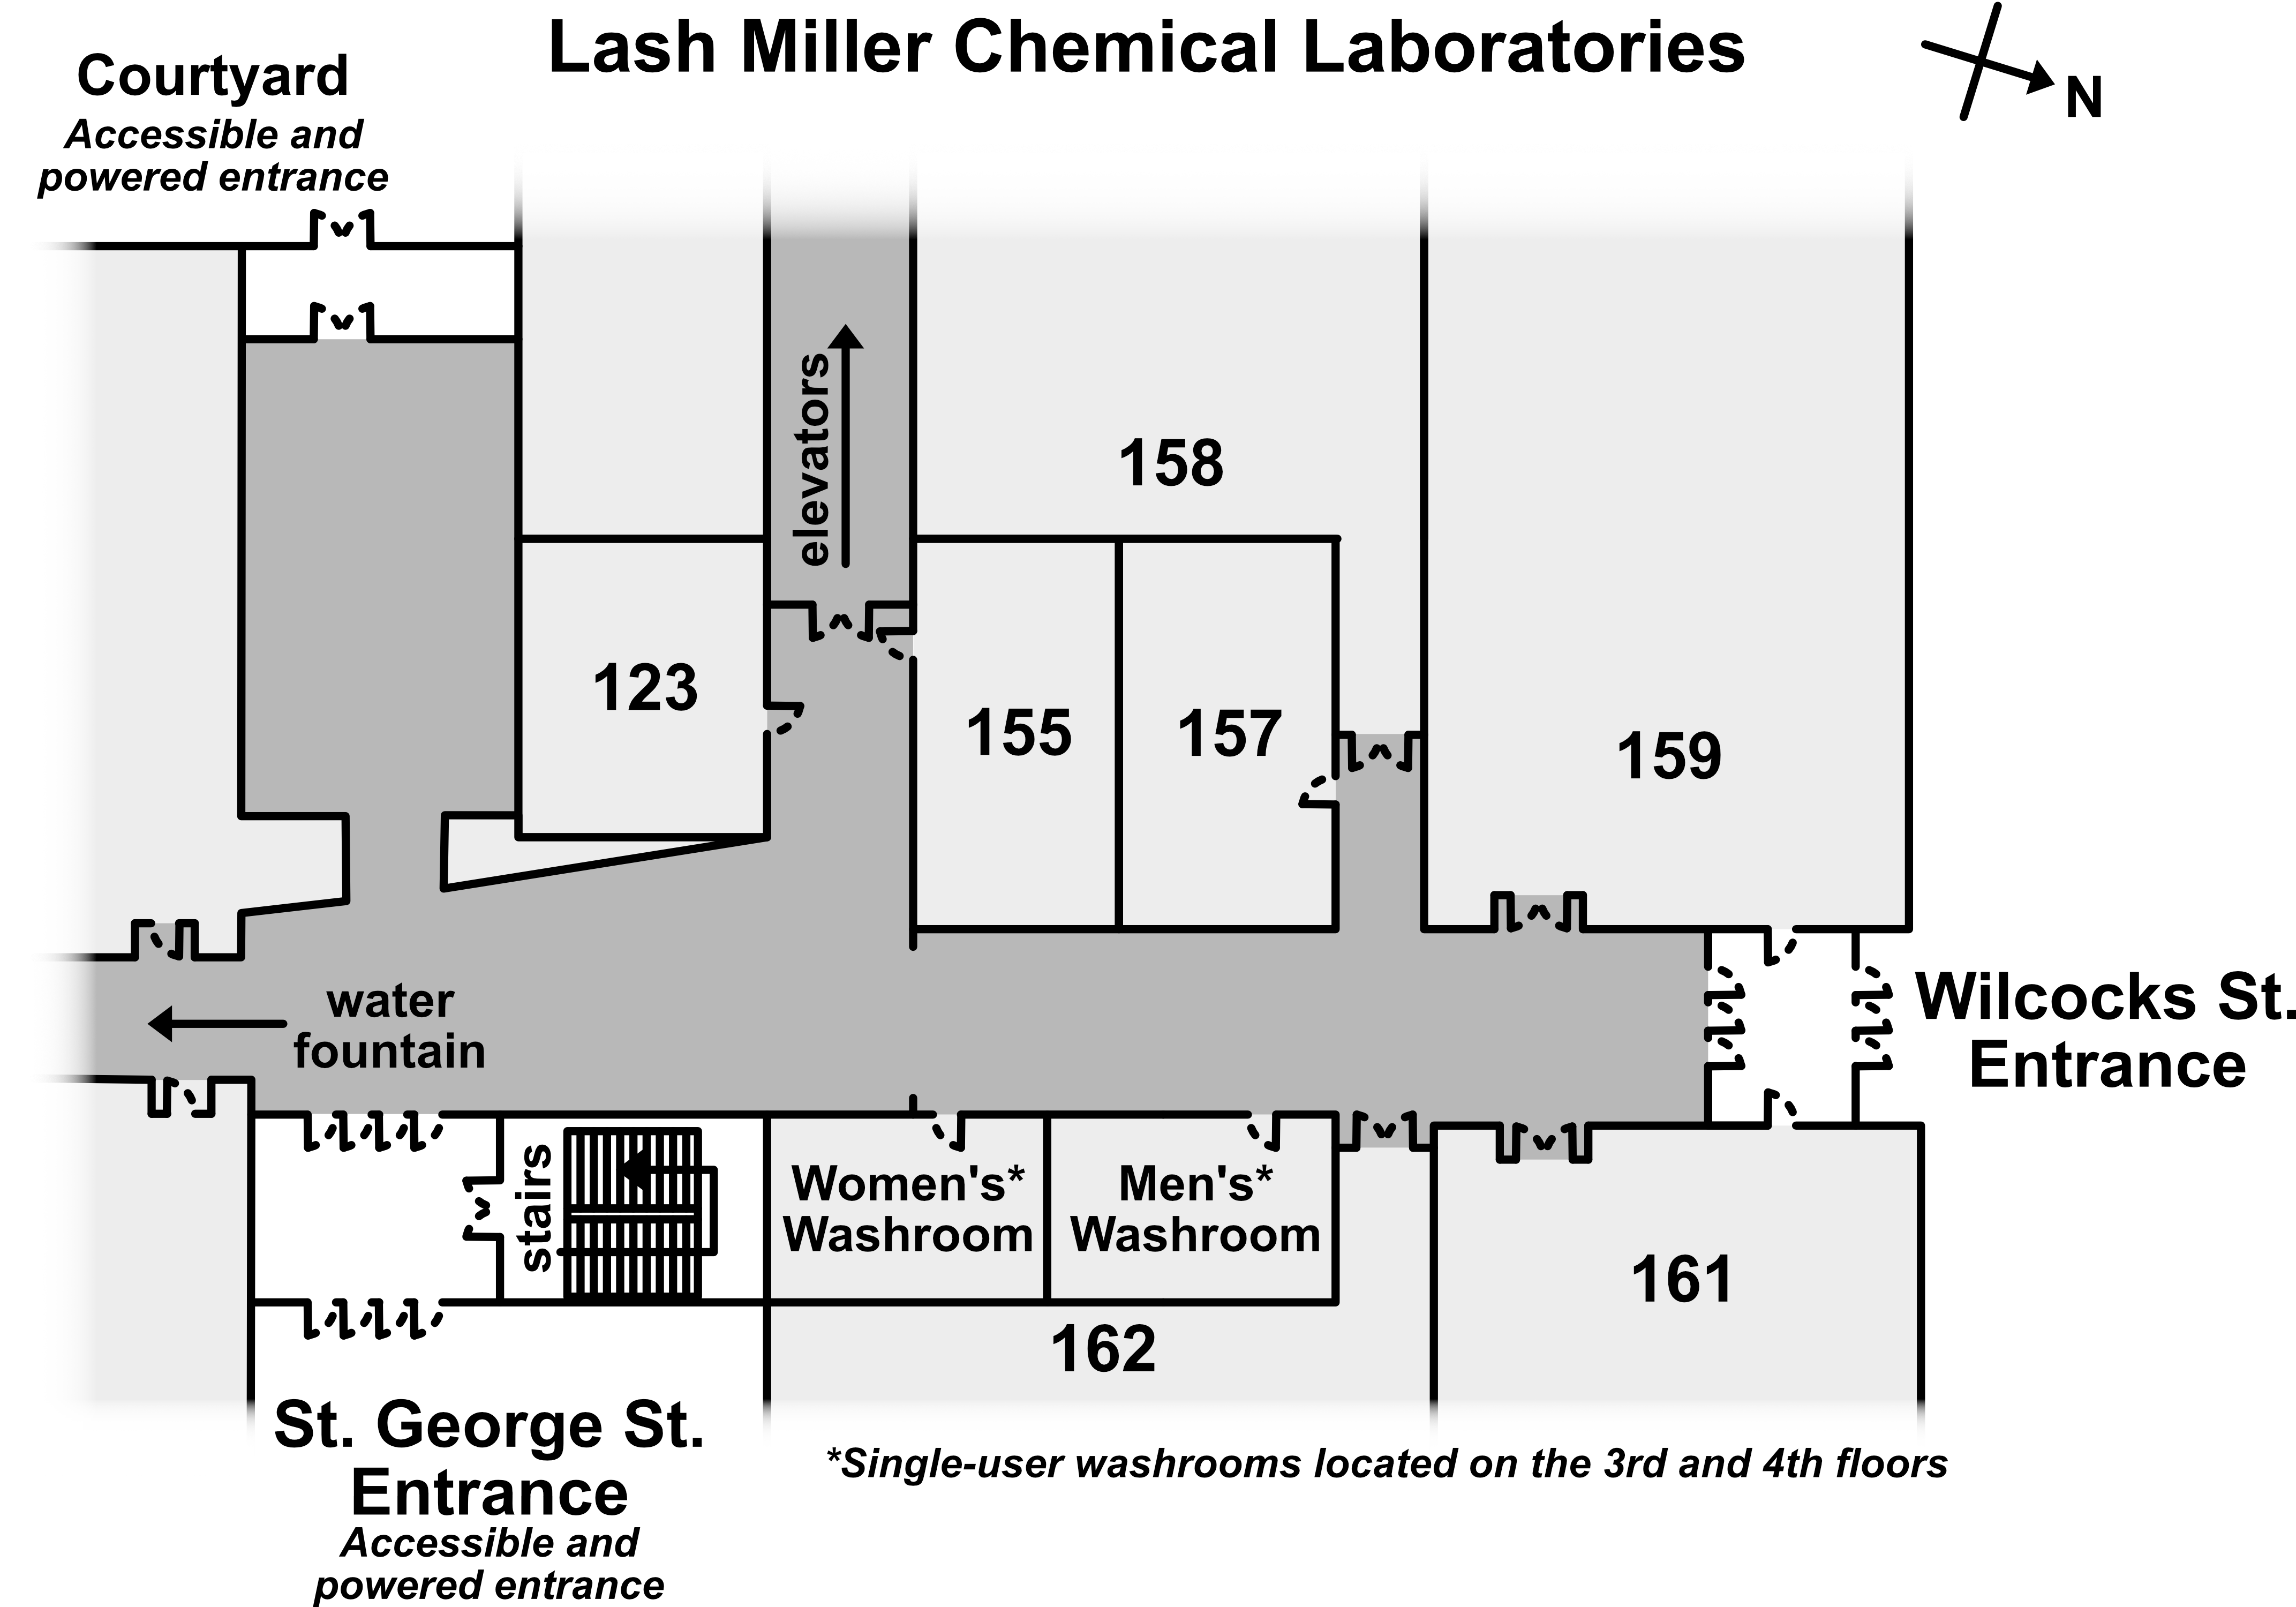
\includegraphics[width=\textwidth,keepaspectratio]{Other_Figures/LM_map.png}
\end{center}
% \vspace{1cm}
% \textbf{A}: 
% Lash Miller, 80 St. George Street \\
% \indent \textbf{Registration, Poster Sessions, Lecture sessions, Workshops, 
% Saturday lunch}\\
% \textbf{B}:
% Lash Miller Chemical Laboratories, Davenport Atrium, 3rd floor\\
% \indent \textbf{Friday dinner}\\
% \textbf{C}:
% Graduate Student Union Pub, upstairs\\
% \indent \textbf{Friday Pub night}

\section*{From Lash Miller (80 St. George St.) to Dim Sum King (421 Dundas St. W)}
\label{conference_to_dimsumking}
\phantomsection\addcontentsline{toc}{section}{\hyperref[conference_to_dimsumking]{From Lash Miller to Dim Sum King}}

\begin{center}
	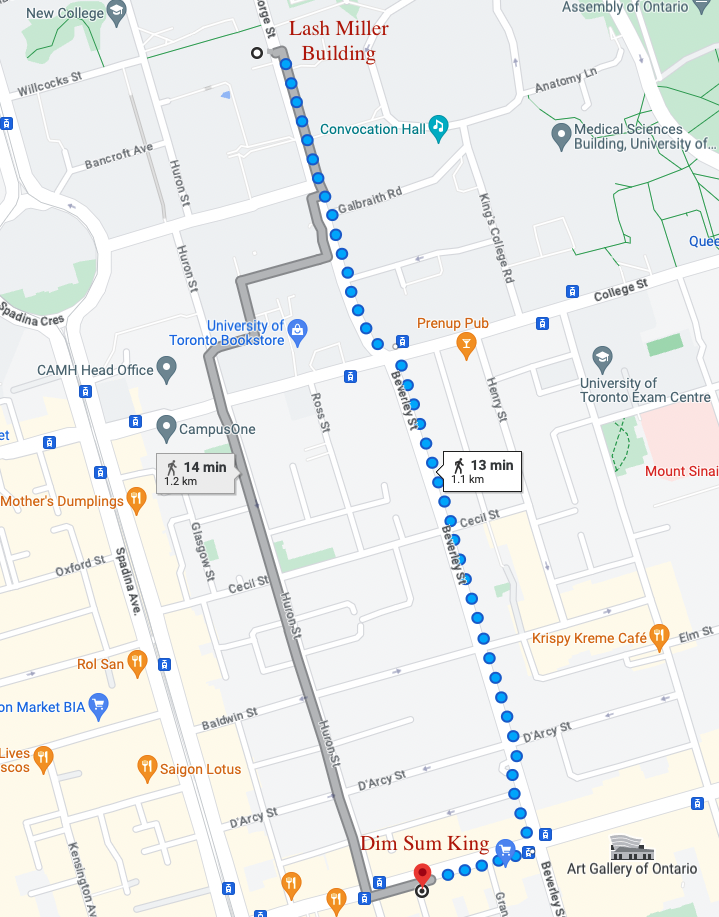
\includegraphics[scale = 0.5]{Other_Figures/map to dim sum king_revised.png}
%\end{center}
\\\vspace{0.5cm}
Exit Lash Miller to St. George St. Walk South (Right)\\
Continue South (street name will change to Beverly St.) until Dundas Ave. \\
Dim Sum King will be half a block to the West (right) on the South side of the street.
\end{center}

\section*{Outside view of Dim Sum King}
\label{Outside View_Of_Dimsumking}
\phantomsection\addcontentsline{toc}{section}{\hyperref[conference_to_dimsumking]{Outside View of Dim Sum King}}

\begin{center}
	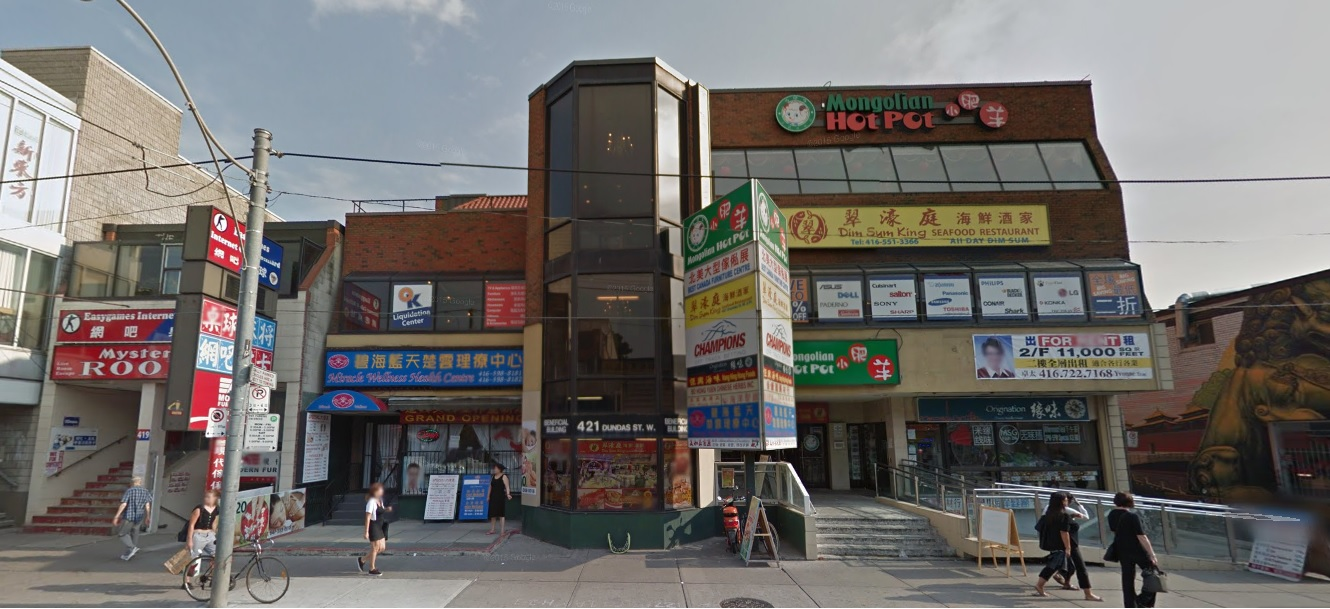
\includegraphics[scale = 0.5]{Other_Figures/Outside View of Dim Sum King.jpg}
\end{center}

%~~~~~~~~~~~~~~~~~~~~~~~~~~~~~~~~~~~~~~~~~~~~~~~~~~~~~~~~~~~~~~~~~~~~
%====================================================================
%~~~~~~~~~~~~~~~~~~~~~~~~~~~~~~~~~~~~~~~~~~~~~~~~~~~~~~~~~~~~~~~~~~~~

\end{document}
